\documentclass[a4paper,notitlepage]{article}

\usepackage[top=2cm, bottom=2cm, left=3cm, right=3cm]{geometry}

\usepackage{amssymb, amsmath}

% This needs to occur before hyperref and minted
\usepackage{float}

\usepackage{multirow}

\usepackage[hyphens]{url}
\usepackage{hyperref}

\usepackage{appendix}
\usepackage[numbers]{natbib}

\usepackage{graphicx, subfigure}
\usepackage{epstopdf}

\usepackage{tabularx}
\usepackage{longtable}

\usepackage{comment}

% Use minted and set the visual style to be the
% same as the one used by visual studio
\usepackage{minted}
\usemintedstyle{vs}

% Allows use of autoref with lables in listings
\providecommand*{\listingautorefname}{Listing}

\usepackage{caption}

\newcommand{\mysideways}[1]{\begin{sideways}#1\end{sideways}}



\usepackage[parfill]{parskip}
\setlength{\parindent}{0pt}
\setlength{\parskip}{0.75\baselineskip}

% A better tilde (~)
\newcommand{\mytilde}{\raise.17ex\hbox{$\scriptstyle\mathtt{\sim}$} }

% For use in the title page
\newcommand{\HRule}{\rule{\linewidth}{0.5mm}}


% For \begin{acknowledgements}
% From: http://www.latex-community.org/forum/viewtopic.php?f=47&t=5464
\makeatletter
\newcommand\ackname{Acknowledgements}
\if@titlepage
  \newenvironment{acknowledgements}{%
      \titlepage
      \null\vfil
      \@beginparpenalty\@lowpenalty
      \begin{center}%
        \bfseries \ackname
        \@endparpenalty\@M
      \end{center}}%
     {\par\vfil\null\endtitlepage}
\else
  \newenvironment{acknowledgements}{%
      \if@twocolumn
        \section*{\abstractname}%
      \else
        \small
        \begin{center}%
          {\bfseries \ackname\vspace{-.5em}\vspace{\z@}}%
        \end{center}%
        \quotation
      \fi}
      {\if@twocolumn\else\endquotation\fi}
\fi
\makeatother


% From: http://nepsweb.co.uk/docs/bnf.pdf
% For writing predicate language productions
\newcommand{\pn}[1]{\langle \textnormal{#1} \rangle}
\newcommand{\pp}{\models}
\newcommand{\oo}{\; \mid \;}
\newcommand{\sk}{\dots }
\newcommand{\ww}{\;}
\newcommand{\nn}{\perp}
\newcommand{\sm}[1]{\textnormal{#1}}
\newcommand{\sd}[1]{\textnormal{\it #1}}

\begin{document}

\begin{titlepage}
\begin{center}

% Upper part of the page

\includegraphics[scale=0.6]{the_warwick_uni_blue.eps}\\[0.75cm]

\textsc{\LARGE Department of Computer Science}\\[1.5cm] 

\textsc{\Large Fourth Year Project}\\[0.5cm]


% Title
\HRule \\[0.4cm]
{\Huge \bfseries Towards Practical Debugging of Wireless Sensor Network Applications}\\[0.4cm]

\HRule \\[2cm]

% Author and supervisor
\noindent{
\begin{minipage}{0.4\textwidth}
\begin{flushleft} \large
\emph{Authors:}\\
Matthew Bradbury (0921660) \\
Tim Law (0918647) \\
Ivan Leong (0830934) \\
Daniel Robertson (0910210) \\
Amit Shah (0904778) \\
Joe Yarnall (0905247)\\
\end{flushleft}
\end{minipage}}
\hfill
\noindent{
\begin{minipage}{0.4\textwidth}
\begin{flushright} \large
\emph{Supervisor:} \\
Dr.~Arshad Jhumka
\end{flushright}
\end{minipage}}

\vfill

\begin{abstract}
Debugging tools are vital for developers to produce reliable software, however traditional tools are less useful when developing software for new system paradigms such as wireless sensor networks. As wireless sensor networks (WSNs) become increasing prevalent in our lives it will become ever more important that the software they are running works reliably and to do this debugging tools will be required. This project investigates how predicates can be specified and checked throughout WSNs and how errors can be reported to a base station. We also investigate deploying these applications not just in a simulator but on hardware in an environment where unexpected failures may occur.
\newline
\newline
\noindent \textbf{Keywords} - Wireless Sensor Networks; Debugging; Reliability; Predicate Checking;
\end{abstract}

\vfill
\vfill
\vfill
\vfill

% Bottom of the page
{\large October 2012 - July 2013}

\end{center}
\end{titlepage}

%No numbering on first and second pages
\pagestyle{empty}
\thispagestyle{empty}\clearpage

\newpage

\begin{acknowledgements}
Acknowledgements
\end{acknowledgements}
\newpage


\pagestyle{plain}
\setcounter{page}{1}

\tableofcontents
\clearpage

% !TeX root = Report.tex
\section{Introduction}

\subsection{What is a Wireless Sensor Network?}

A wireless sensor network, or WSN for short, is a collection of networked sensors called Motes; these sensors are capable of short range wireless communication and they have the ability to sense their surrounding environment\cite{Mica2002,TankBible}. The network forms a distributed system that can perform a variety of distributed algorithms, usually data gathering and similar tasks. To communicate, each node is equipped with a radio that allows them to send and receive messages to neighbouring nodes within a limited range. To sense the environment motes typically have a range of embedded sensors such as heat, light, humidity and many others. They typically contain a simple central processing unit (CPU), which is programmed to control the hardware on the motes. The CPU also processes events which are triggered by the hardware (such as messages being sent and received) and it also handles any other computation necessary for the operation of the system. As the platform is designed to be mobile the motes do not operate on a mains power supply, instead they run off stored energy in a battery. WSNs is a field of Computer Science that is currently the focus of much research and wireless sensor networks have a wide range of practical applications that stretch from battlefield intelligence for the military\cite{?} to industrial process monitoring for manufacturing companies\cite{?}.

A defining characteristic of designing applications for wireless sensor networks is the restricted and finite energy supply available to each node. Therefore, wireless sensor nodes tend not to use expensive broadcasting protocols such as IEEE 802.11 \cite{Mica2002}, but instead use much simpler alternatives to save energy. For example wireless protocols such as IEEE 802.15.4 ZigBee \cite{1253873, 4014617} are designed to be used by wireless sensor networks and have a lower energy usage associated with them. Some applications rely on even lower level behaviour specified by a certain MAC layer \cite{5751321,4469515,?,BMAC,SMAC,XMAC}, these applications involve a trade-off between development time and energy usage. Where simplicity is often sacrificed for decreased energy usage. Using these simple protocols unfortunately has the downside of meaning that broadcasts are subject to several types of collisions and message losses. So it is very important that the software running on the nodes is designed to handle these cases. Being battery powered means that development of applications for Wireless Sensor Networks is fundamentally limited to maximising the system's lifetime so that the highest utility can be achieved from the network.

As wireless sensor nodes operate in harsh outdoors condition\cite{SzewczykPMC04, Werner-Allen:2006:FYV:1298455.1298491}, there is a high probability of them failing. These faults can range from hardware damage caused by environmental conditions or tampering, software bugs, or simply a denial of service caused by nodes running out of power. So algorithms and software need to be designed to handle these potential failures, otherwise they risk catastrophic failure when they encounter these issues.

Wireless sensor nodes are designed with the intention for them to operate in remote and traditionally unreachable locations with no human input for the lifetime of their operation\cite{1437066}. Given this a defining characteristic of a WSN system is that any applications developed for it must be self-configuring in nature; this is, the system must be able to organize itself and the network with no external input\cite{?}. Evidently, solutions to this issue are often considered hand in hand with the problem of network robustness and fault tolerance.   

While a limited energy source, self-configuration and network robustness are the predominant characteristic of a wireless sensor node, there are numerous other traits or issues that can be considered. For instance it is possible for these nodes to be mobile (for example an ad-hoc network of PDAs or motes built into soldiers helmets) \cite{4224091}, this can lead to very interesting behaviour in handling communication between these nodes.

%TODO: MORE OBSCURE WSN BEHAVIOUR CONSIDERATIONS

\subsection{The Problem - Debugging Distributed Systems}

Developing a distributed system is considered a particularly challenging task, more so than a traditional application, there are several reasons for this. Firstly, Within a distributed system multiple processes must execute in parallel, this means that variables may be updated independently or in repose to other processes which can lead to a myriad of synchronisation and timing issues that the developer must account for. Secondly, traditional programming languages are not well suited to develop distributed programs\cite{93692,345131}.

In any system, software or otherwise, developed by humans there is the potential for mistakes. Mistakes can be benign or they can cause unintended behaviour and system failures. Developing tools to detect these \emph{bugs} and notify the developer so they can be corrected is an incredibly important part of any toolchain. For example the GNU toolchain has utilities such as gdb\cite{?}, this allows developers to place breakpoints in code which will halt the programs execution at that state so that it can be examined. There are also numerous other tools that look for memory issues (valgrind\cite{?}), security flaws (TOOL NAME\cite{?}) and many other classes of bugs.

Developing distributed systems is a difficult task; however, debugging these systems can be even more challenging\cite{345131}. When considering a distributed system if you want to examine the state of a system at a given point you cannot simply set a breakpoint in your local binary. The solution to this debugging is non-trivial, this is due to the difficulties that arise from distributed systems being non-deterministic in nature due to message communications \cite{?}. Be it when the message started transmission, how long it took, if it succeeded or in what order transmissions occurred. So every time a distributed program is run it is possible for a different result to be obtained, due to the different order of execution. This goes against one of the usual assumptions of debugging traditional applications where it is assumed that one execution with a set of inputs will execute in exactly the same way again with the same set of inputs\cite{?} (i.e. determinism).

As the execution may be different each time in a distributed system it is not suitable to wait for a bug to occur, and then try to work out where it is. Rather, the system needs to be self-evaluating its state as it executes the distributed program; if a fault is detected, then the debugging tools will report the issue. One way to do this it to test if the system satisfies some global predicate, of which there has been much work to find and check different classes of these predicates \cite{553309,345831,277788}. However, of all the work that has been done, little of it has focused on wireless sensor networks where an important focus is perhaps the trade-off between accuracy and the report-ability of a predicate with the aim of reducing energy usage. In this paper we will discuss our development of just such a set of tools, we intend to focus on developing a system that can accurately evaluate predicates and provide useful information about real sensor networks running outside of a simulator.

\subsection{Related Work - New Lit Review???}

\subsubsection*{Fault-Error-Failure Cycle - NEEDS WORK}

It should be clear that the types of predicates are important to consider when developing a predicate checking mechanism. Also important are the types of errors that these predicate checking algorithms can detect. To understand this it is first important to understand how errors can arise, which can be done by examining the fault-error-failure cycle. This cycle says that a \emph{fault} once caused by either some external influence (e.g. radiation leading to bit-flips in memory \cite{1017791}) or internal influence (e.g. code bugs) will lead to an \emph{error}, this is the \emph{activation} step. An error is the manifestation of the fault (e.g. memory holding the incorrect value). An error then leads to a \emph{failure} in the step called \emph{propagation}, the failure of the system is an observable deviation from the system's specification (e.g. allowing doors to be opened that should remain closed). It is not always the case the faults lead to errors, or errors lead to failures, sometimes multiple faults or errors are respectively required to cause a single error or failure. \cite{1335465}

There is a choice of what should be measured and checked in predicates; should faults, errors or failures be measured? Faults cannot be measured \cite{?} in a way that is possible for a mote, so they are discounted. That leaves measuring errors and failures. Typically failures would be the event being measured \cite{?} as that is what arises after an error actually causes the issue to happen. However, errors can also be measured if there is a dedicated program checking the state and comparing it to an expected state \cite{?}. For example an ECC (error correcting code) such as a Hamming Code can be used to detect and correct an error (in this case a bit-flip) in some memory after a fault (such as a voltage surge ) \cite{hamming1950error}.

Much of what has been discussed has involved transient faults such as those caused by environmental conditions, however, there is a class of faults that are a lot more common and much easier to resolve - faults caused by software bugs. These faults can lead to programs ending up in the wrong state and performing incorrectly. There has been a certain amount of work that looks into detecting traditional distributed system bugs (such as deadlock \cite{5587352,5284172}) in wireless sensor networks. However, there has been little work in looking into providing tools to aid in system debugging.

\subsubsection*{Classes of Distributed Predicates - NEEDS WORK}

To begin with it is important to understand what predicates are relevant to distributed systems. First off we have a distinction between global and local predicates, global predicates involve taking a consistent global snapshot of the system and checking whether the snapshot satisfies the global predicate \cite{277788} and local predicates instead work with a subset of the network \cite{553309}. These predicates have also have a notion of stability, a stable predicate will remain true once it has turned true (e.g. termination), whereas unstable predicates can alternate between true and false. Finally there is a distinction between weak and strong, where a weak predicate holds if there exists an observation where the predicate is true and a strong predicate holds if it is true for all observers of the distributed computation\cite{553309,Cooper:1991:CDG:127695.122774}. Knowing what classes of predicates there are is important because when checking certain properties of a system a certain class of predicate will be required and thus a certain implementation will be needed to ensure the predicate is correctly checked. An example of this is when running an algorithm using global snapshots to detect stable predicates, that same application may not be suitable to detect unstable predicates because the predicate could switch to false and then back to true before the next snapshot.

\subsubsection*{Existing Sensor Network Predicate Checking Tools}


\subsubsection*{Practical Sensor Network Deployments}




\clearpage

% !TeX root = Report.tex
\section{Literature Review}

\subsection{Routing in Sensor Networks}

\cite{TankBible}
\cite{Akkaya2005325}

%Aggregation:
\cite{aggphdfeng} % http://ecommons.usask.ca/bitstream/handle/10388/etd-06292010-135305/thesis-jie.pdf

\subsubsection*{Flooding}

\subsubsection*{Tree Aggregation}
\cite{1628365} % https://ieeexplore.ieee.org/xpl/login.jsp?tp=&arnumber=1628365

\subsubsection*{Clustering}

S'pose I'd best do this one - Giles
\cite{LEACH}\cite{placement}\cite{SECC}\cite{EEMC}

\subsection{Simulating Sensor Networks}

\subsubsection*{TinyOS}

TOSSIM \cite{levis2003tossim}

\subsubsection*{Contiki}
% Cite basically all the papers at: http://www.contiki-os.org/support.html

\paragraph{A Database In Every Sensor} 
\cite{Tsiftes:2011:DS:2070942.2070974} %http://dunkels.com/adam/tsiftes11database.pdf
\cite{TinyDB}

\paragraph{Sensor Network IP Stacks}
\cite{ko2011beyond} % http://dunkels.com/adam/ko11beyond.pdf
\cite{dunkels2009efficient} % http://dunkels.com/adam/yazar09efficient.pdf
\cite{Durvy:2008:MSN:1460412.1460483} %http://dunkels.com/adam/durvy08making.pdf
\cite{dunkels2003full} % http://dunkels.com/adam/mobisys2003.pdf

%Bring into interoperability with the Internet of Things
\cite{Christin_Reinhardt_Mogre_Steinmetz_2009}

\paragraph{Cooja / MSPSim}
\cite{Eriksson:2009:CIT:1537614.1537650} % https://dl.acm.org/citation.cfm?id=1537614.1537650

\paragraph{Protothreads}
\cite{Dunkels:2006:PSE:1182807.1182811} % http://dunkels.com/adam/dunkels06protothreads.pdf

\paragraph{Energy Estimation}
\cite{Dunkels:2007:SOE:1278972.1278979} % http://dunkels.com/adam/dunkels07softwarebased.pdf

\paragraph{RIME}
\cite{Dunkels:2007:ACA:1322263.1322295} % http://dunkels.com/adam/dunkels07adaptive.pdf

\paragraph{Beacon Coordination}
\cite{Dunkels:2011:ALB:1966251.1966270} % http://dunkels.com/adam/dunkels11announcement.pdf

\paragraph{Run-time Reprogramming}
\cite{Dunkels:2006:RDL:1182807.1182810} % http://dunkels.com/adam/dunkels06runtime.pdf

\subsubsection*{NS2}

\subsubsection*{JProwler}

\subsubsection*{Simulating Energy Consumption}
\cite{Shnayder04}


\subsection{Sensor Network Platforms}

\subsubsection*{MICA}
\cite{Mica2002}

\subsubsection*{Sky}


\subsection{Practical Experience in Sensor Networks}
\label{sec:lit-review-practical-experience}

\subsubsection*{Habitat Monitoring}

Habitat monitoring is widely thought to be one of the key wireless sensor network application that is driving research and adoption. The problem involves determining the location of the sensor nodes, which then allows tracking \cite{Cerpa:2001:HMA:844193.844196} and two of the primary problems in sensor networks: data aggregation and energy efficient multihop communications.

The research undertaken by \citeauthor{SzewczykPMC04} in \cite{SzewczykPMC04} involves deploying sensor nodes on the Great Duck Island in order to test the long term real-world deployment of sensor networks. The importance of deploying and testing a WSN in the real world is due to the fact that challenges are encountered that are not present in indoor deployments or simulations. The problem becomes one of not just what software needs to run and how, but also consider on what hardware in what conditions. For example the authors wished to waterproof the mote in order to ensure that it survived dew, rain and flooding. However, when enclosing the motes it was worried that (i) radio transmissions would be interfered with and (ii) sensor data could be affected.

Overall, the deployed motes performed well (logging 1.1 million readings over 123 days), however, there were a number of abnormal results that included: (i) sensor readings outside their range, (ii) ``erratic packet delivery'' and (iii) failure of motes. The authors point out (in section 2.5) that in the future it would be useful to augment applications with the ability to notify that failures occurred and to perform self-healing.

The performance of the network showed that initially packet loss was up to 20\% but that slowly decreased, most likely due to the fact that the size of the network network was reducing over time (as nodes permanently crashed). Due to the low network utilisation (under 5\%) \citeauthor{SzewczykPMC04} initially believed that collisions would not play an important role, however, their results suggested otherwise. Their results suggest that this was caused by clock drift which lead to slot assignments not preventing collisions within their period. This importance of clock drift on TDMA-based MAC protocols is something that would tend not to be found from testing in a simulator because of the slow speed of simulation and the length of time it takes for these small clock drifts to lead to an effect.

Overall, one of the major conclusions of this work is that anomalous sensor data can be used to predict mote failures with a high degree of accuracy. The authors believe that this prediction allows for a high level of pro-active maintenance, and self-organisation and self-healing of the network.

\subsubsection*{Animal Monitoring}
% https://www.princeton.edu/~mrm/ZNetASPLOS.pdf
% http://citeseerx.ist.psu.edu/viewdoc/download?doi=10.1.1.14.6467&rep=rep1&type=pdf

Instead of monitoring the habitat, why not simply directly monitor the animal in question? This is the track that a number of other wireless sensor networks have taken \cite{Juang:2002:ECW:635508.605408}. The traditional technique was to attach collars that emit radio waves that are used in manual triangulation or take GPS measurements and then recover the hardware attached to the animal to extract the data. Sensor networks provide a way to extract this data automatically in a much easier manner and can also allow for data to be accessed earlier.   Much of what is true for habitat monitoring is also true for monitoring animals: the hardware needs to be protected against the weather, the data needs to be extracted as reliably as possible and the battery should last as long as possible to make the deployment cost effective.

ZebraNet by \citeauthor{Juang:2002:ECW:635508.605408} in \cite{Juang:2002:ECW:635508.605408} investigates these issues as well as some of the unique deployment issues related to mounting hardware on animals. For example it is very important that the hardware is light enough for the animal to handle for a long time. This adds a new type of trade-off, when considering energy usage and reliability system developers must also consider weight.

Aside from the usual issues associated with sensor networks, having sensors attached to animals presents another very important problem that needs to be solved. Many of the animals that we wish to monitor, are desired to monitor for very good reasons. Most often it is the case that they are endangered or are often the victims of poaching \cite{?}. By attaching wireless devices that broadcast information, it has been found that attackers can trace their way back to a source. There has been much research to develop ways to mitigate this problem, one example is using fake sources to lure an attacker in an alternate direction than that of the real source \cite{Ozturk:2004:SPE:1029102.1029117,Kamat.1437121,6296046}. These additional problems that arise as side-effects of communicating through a wireless medium are often difficult and expensive (in terms of energy) to overcome.



\subsubsection*{Air Pollution}
\cite{libeliumAirPollution}
\cite{wsnpollution} 

\cite{fotuewsnpollution} Claimed: Ivan

Air pollution has been a growing concern in congested urban cities as a result of industrialisation and heavy transportation. These concerns include poor air quality and visibility and long term damaging of human health. Traditional methods of air quality monitoring involving quality control stations are expensive and provides low resolution sensing since monitoring stations are less densely deployed. Wireless sensor networks can be used as an urban monitoring system as it has the advantages of being small, easy to set up and inexpensive with real time monitoring capabilities. Sensors which have the ability to measure a wide range of meteorological data such as rainfall, wind speed, temperature, humidity and concentration of pollutants can be deployed in areas of high population density of vehicles and industrial areas. Collected data is transmitted back to the base station via a global system for mobile communication.

\citeauthor{fotuewsnpollution} in \cite{fotuewsnpollution} proposed a Wireless Mesh Network to establish internet connectivity and simultaneously measure air pollution in Sub-Saharan African cities. These cities experience the most problems due to the increase of industry, domestic waste and fuel combustion and that many chemical industries have been established in the central urban areas. However, with poor infrastructure and telecommunication links in Africa, it would be difficult to deploy a sensor network that will measure air pollution since some pollution areas are out of range of the communication service. In addtion, some polluted areas lack the security measures or have industrial restrictions to deploy fixed sensors so they had to use mobile sensors which were attached on vehicles. 

\paragraph{WSN Challenges}

\begin{itemize}
\item Reducing communication interference

High-gain antennas was used to reduce the probability of interference from non-city radio frequency emitters such as WiFi and access points. However, interference may also be caused from inter-device communication and was reduced by using multiple orthogonal channels. Each set of devices would use a unique channel to communicate with a different set of devices for example the mesh network would use a channel Cs with the sensors and channel Cg with the gateway.

\item Limiting number of request messages each sensor can receive from the data server.

The network uses an Ad-hoc On-Demand Distance Vector routing protocol for efficient forwarding of data packets to the data server and makes use of a series of messages to communicate through the network and to discover and maintain data routes. A request message is propagated to the network when the data server requests for a specific data item. All the sensors receives the message and checks whether is it the destination or not. If not, it stores a copy of the message in its buffer containing previously broadcasted request messages and rebroadcasts it back to its neighbours. Once the destined sensor receives the message it sends back a reply message using the reverse path of the data server.

To prevent the sensors from overloading with request messages, each message is set with a Time-To-Live (TTL) value with discards the message when the value expires. This value is dependant on the size of the network where a larger network will have higher TTL value to ensure that the request messages reaches the defined destination.

\item Energy Usage

The wireless mesh network is energy efficient since the sensors are energy constrained. This uses an enhanced energy conserving routing protocol which employs a routing algorithm that aims to distribute data among maximally disjoint paths towards the sink so that the lifeline of the WSN service can be prolonged. It also allows the sensors to participate in carrying the global traffic over the network

\item Data transmission periods

To avoid high energy consumptions, data from the sesors to the data server were only transmitted at specifc times of the day (non-real time). This allowed for energy and bandwidth optimization and thus increasing the network's lifetime on the long run.

\item Optimized placements of mesh router 

Since the network includes mobile sensors, there are chances that it can lose connectivity with the the fixed sensors. A challenge that the team faced was placing the mesh routers in such a way that they were always connected to the mobile and fixed sensors in order to receive the sensed data. This is crucial for network reliability and quality of service.
\end{itemize}



\subsubsection*{Forest Fires}
\cite{libeliumForestFires}
\cite{FireWxNet}
\cite{4428702}

\subsubsection*{Volcano Monitoring}
Claimed: Ivan

Active volcanoes need to be monitored to predict the likelihood of future eruptions so that early-warning signs can be issued for the evacuation of habitants near the volcano. Today, volcanoes use wired arrays of sensors such as seismometers and acoustic microphones to collect seismic and infrared (low-frequency acoustic) signals and determining a wide range of factors such as sources of volcanic eruptions, interior structure of a volcano and differentiating eruption signals from noise. A typical study can indlue the placement of several stations around the volcano where each contains a low distribution of wired sensors that collects data to a hard drive. Data is then collected manually in a possibly inconvenient location.

To address the issue of high power consumption of these wired sensors, \citeauthor{Werner-Allen:2006:FYV:1298455.1298491} in \cite{Werner-Allen:2006:FYV:1298455.1298491} introduced the deployment of embedded wireless sensor networks consisting of low-power nodes with minimum CPU, memory and wireless communication capabilities. This allows for long distance real time monitoring of volcanic activities and reducing the need for manual data collection. The main challenge however is that environmental monitoring studies sample at a frequency which is much lower than the sample rate of volcanic time series. This is due to the limited radio bandwidth of the sensors thus requiring the need for efficient power management techniques and accurate time synchronization of the nodes. 

\citeauthor{Werner-Allen:2006:FYV:1298455.1298491} implemented a wireless sensor network that was deployed on the Volcano Tungurahua in central Ecuador using a Mica2 sensor mote platform and three infrasonic microphone nodes. These nodes transmitted data to an aggregation node, which relayed the data over a 9km wireless link to the base station. Time synchronization for the infrasonic sensors was done using a GPS receiver which receives a GPS time signal and relays the data 
to the infrasound and aggregator nodes. Over a period of time, the temperature and battery voltage may change and this may affect the sampling rate of the individual nodes and the precision of the time recorded from the GPS time stamp message. These uncertainties was addressed by applying a linear regression to the logged data stream giving an estimation of the node outputs. In addition, the sensor nodes where required to be protected against harsh environments such as rain and long exposure of sunlight by using waterproof pelican cases and 1/4-wave whip antennas.

Their first deployment on the volcano included a small network where nodes could send continuous signals to each other, however this was not feasible for a larger network deployed over longer periods of time. To solve the issue with bandwidth and energy consumption, the team implemented a distributed event detector which only transmits well-correlated signals to the base station. A local event detection algorithm is used to trigger data collection for uncorrelated signals.

\begin{itemize}
\item Distributed Event Detector

To measure the correlated signal, the distributed detector uses a decentralized voting system among a group of nodes. Each nodes samples data at a continuous rate of 102.4Hz and buffers a window of such data while running a local event detection algorithm. If an event is triggered it uses a local radio broadcast to broadcast a vote to other nodes and a global flood to initiate global data collection from all the nodes. Radio contention is reduced using a token-bases scheme for scheduling transmission, where each nodes transmits their buffer one after the other. 

\item Local Event Detector

The team implemented two local event detectors; a threshold-based detector and an exponentially weighted moving average (EWMA)-based detector. The former is triggered when the signal rises above an upper threshold and below a lower threshold. However due to spurious signals such as wind noise, the detector may be susceptible to false trigger. On the other hand, the EWMA detector calculates two moving averages with different gain parameters and is triggered if the ratio of the two averages and the new sample exceeds some threshold T. This method is less affected by node sensitivity and any duplicate triggers over a window of 100 samples are suppressed.
\end{itemize}

\paragraph{Data Collection and Performance}

During the deployment, the team managed to log 54 hours of continuous data which includes seismoacoustic signals from several hundred events. The raw data was used to analyse the system's performance and many challenges where discovered in the early observations. They discovered that on average only 61 percent of data was retrieved from the network and on several occasions the modems which transmitted data back to the station would experience short drop-outs, causing all data aggregated from the nodes to be lost. In addition, duplicate packets were also recorded as a likely result of redundant retransmission and lost acknowledgement. Both lost and duplicate data had to be accounted for before being stored in the timebase.

\paragraph{Conclusion and Improvements}

In general, the event-triggered model was successful in detecting eruptions and other volcanic events and was able to verify the working of the local and global event detectors by examining the downloaded data. However, since the experiment was deployed over a limited area space of the volcano, further work is to be done to instrument volcanoes at a larger scale. This includes, and most importantly, the management of energy and bandwidth usage of the sensors and increasing its computational power to deviate from continuous data collection to enabling the collection of well-correlated signals. 

\subsubsection*{Structural Monitoring}
\cite{5508230}

\subsubsection*{Development of Applications}
\cite{Fagerstrom:1988:DTD:55823.55833}


\subsubsection*{Power Considerations}


\subsection{Predicates}

Before we can consider what predicates we can try to check for, or how we should check those predicates, we first need to understand what we are detecting and why. In dependable systems we need to consider the fault-error-failure cycle. This cycle says that a \emph{fault} once caused by either some external influence (e.g. radiation leading to bit-flips in memory \cite{?}) or internal influence (e.g. code bugs) will lead to an \emph{error}, this is the \emph{activation} step. An error is the manifestation of the fault (e.g. memory holding the incorrect value). An error then leads to a \emph{failure} in the step called \emph{propagation}, the failure of the system is an observable deviation from the system's specification (e.g. allowing doors to be opened that should remain closed). It is not always the case the faults lead to errors, or errors lead to failures, sometimes multiple faults or errors are respectively required to cause a single error or failure. \cite{1335465}

There is a choice of what should be measured and checked in predicates, should faults, errors or failures be measured? Faults cannot be measured \cite{?} in a way that is possible for a mote, so they are discounted. That leaves measuring errors and failures. Typically failures would be the event being measured \cite{?} as that is what arises after an error actually causes the issue to happen. However, errors can also be measured if there is a dedicated program checking the state and comparing it to an expected state \cite{?}. For example an ECC (error correcting code) such as a Hamming Code can be used to detect and correct an error (in this case a bit-flip) in some memory after a fault (such as a voltage surge ) \cite{hamming1950error}.

Much of what has been discussed has involved transient faults such as those caused by environmental conditions, however, there is a class of faults that are a lot more common and much easier to resolve - faults caused by software bugs. These faults can lead to programs ending up in the wrong state and just performing incorrectly. There has been a certain amount of work that looks into detecting traditional distributed system bugs (such as deadlock \cite{?}) in wireless sensor networks. However, there has been little work in looking into providing tools to aid in system debugging. The rest of this section will cover work on predicates in sensor networks, including detection of them and methods for identifying why is system is not performing correctly.


\subsubsection*{Global Predicate Detection}

Perhaps one of the most well known techniques to undertake this kind of debugging is Global Predicate Detection (GPD). GPD involves ``taking a consistent global snapshot of the system and checking whether the snapshot satisfies the global predicate'' \cite{277788}. These snapshots are repeated periodically and checked if they satisfy the predicate, in doing so properties can be detected that are required for the predicate to hold.

However, GPD is not as simple as this. To begin with there are two types of global predicates: stable and unstable. Stable predicates are ones that remain true once they become true \cite{277788} and unstable predicates can fluctuate between true and false. An example of a stable predicate is termination, once a system has terminated it cannot turn it self back on again. There also exists a distinction between strong and weak predicates, where strong predicates hold for the entire network ($definitely : p$) and weak predicates hold for a subset of that network ($possibly : p$) \cite{553309,345831}. Because of the unreliability of wireless networks it may often be the case that all that can be said is that the predicate is possibly true, due to not receiving all the information that is required to evaluate the predicate \cite{?}.


\subsection{Predicate Detection or Checking in Distributed Systems}

\subsubsection*{NodeMD}
\cite{NodeMD}


\subsubsection*{Debugging by Computing Aggregates}
% https://ieeexplore.ieee.org/xpl/login.jsp?tp=&arnumber=1203364
\cite{1203364}

\subsubsection*{Sympathy}

One of the projects that is summarised by \citeauthor{herbert2007adaptive} in \cite{herbert2007adaptive} is a method for identifying and localizing failures called Sympathy \cite{ramanathan2005sympathy}. Sympathy is intended to be run either in pre- or post-deployment environments where it collects data from distributed nodes at a sink. When insufficient data is received it is taken to imply that there exists a problem (insufficient data is component defined). The idea is that by monitoring data (both actively and passively) between components the system can identify what kind of failure occurred in a certain area of the network. Both of which are very useful when trying to debug a failure.

It does, however, have some downsides. The first is that there is assumed to be no traffic and thus no application traffic or network congestion. These are real issues especially when applying this kind of debugging to a high throughput sensor network. There are also a number of spurious failure notification, which the authors are working on reducing, by applying a Bayes engine.

\subsubsection*{DICAS: Detection, Diagnosis and Isolation of Control Attacks in Sensor Networks}

Detection, Diagnosis and Isolation of Control Attacks in Sensor Networks (DICAS) \cite{dicaspaper} is a lightweight distributed protocol for Wireless Sensor Networks that mitigates the effects of a wide-range of control traffic attacks. DICAS does this by utilizing a unique property of a wireless sensor network, this is that each node is able to monitor a part of their neighbours network traffic. Using DICAS the authors were able to create LSR a lightweight secure routing algorithm for Wireless Sensor Networks.

In DICAS nodes maintain a data structure of their first hop neighbours for local monitoring to detect malicious nodes and in local response to isolate these nodes. When a node is deployed it finds and authenticates all of its 1 hop neighbours using a pairwise shared key. These neighbours communicate their neighbours, 2 hop neighbours to the original node, and their own commitment key, which is generated using a random seed, to the newly deployed node. Each node will then have knowledge of all of its 1 hop neighbours as well as their commitment keys and all of its 2 hop neighbours.

Using this knowledge the DICAS protocol can enact a collaborative detection strategy where every node monitors the traffic going in and out of it's neighbours. Each node that is within transmission range of both the sending(X) and receiving(A) nodes of a packet are considered guard nodes of A over the link from X to A. These nodes maintain a watch buffer of packets sent from X to A, the duration and information stored are determined by the attack type under consideration by the system. Each guard node maintains a malicious counter for each link it is monitoring, if A drops, delays, changes or fabricates a packet from X then the guard node will increase its malicious counter. If the malicious counter exceeds a predefined threshold the node is considered to be malicious and is removed from the neighbours list. The guard node propagates this knowledge to all the other nodes in its neighbour list. When another node receives enough authenticated alerts about the malicious node it is excluded from its neighbours list. Once all 1 hop nodes have excluded the malicious node then it is effectively isolated from the system and all packets from or to that node are ignored.      

The authors tested the DICAS algorithm against 5 sets of attacks, these are:
\begin{enumerate}

\item Route Traffic Manipulation

\item ID Spoofing and Sybil Attacks

\item Wormhole Attacks

\item Sinkhole

\item Rushing Attack

\end{enumerate}

Additionally, the paper describes a cost analysis on the DICAS algorithm, these are the results: 
\begin{itemize}
\item Memory Overhead

The memory overhead is the most pressing of the overheads created by the DICAS algorithm. The algorithm must store several data structures on each node: a neighbours list, a watch buffer, a commitment key list and the alert list. These structures are variable on sizes dependent on the number of nodes in the network, the network layout and the MAC layer delay for acquiring a channel. Any implementation must consider the memory cost of the algorithm seriously.

\item Computation Overhead

With regards to computation they found that each packet received or sent required: one lookup for the current source and destination in the neighbour list, for an incoming packet - adding an entry to the watch buffer or for an outgoing packet - deleting an entry from the watch buffer. Since the size of the watch buffer and the neighbour list structure are relatively small, the computation time required for these operations is negligible.

\item Bandwidth Overhead

When considering bandwidth the overhead was primarily gained in 2 conditions: after node deployment when a node is populating its neighbour list and during a wormhole attack detection where a node is informing its neighbours of the malicious node. However, these cases make up a negligible fraction of the total network traffic over the lifetime of a wireless sensor network.
\end{itemize}

\subsubsection*{H-SEND: Hierachichal SEnsor Network Debugging}

H-SEND is a framework for detecting faults in WSNs, designed to minimise energy consumption. It differs from related algorithms by being capable of handling very large WSNs. \cite{herbert2007adaptive}

There are 4 main steps involved in H-SEND:

\begin{enumerate}
	\item Developer specifies invariants when writing the software
	\item Invariant checking code is (semi--)automatically inserted during compilation
	\item If an invariant is violated at runtime, actions are taken (such as increased logging frequency, or an error message to the base station)
	\item Developer can use the information to fix the software, and then upload the patched version
\end{enumerate}

There are a variety of different types of invariants that can be specified, typically characterised by the following three dichotomies:

\begin{itemize}
	\item Local vs. Multi--node invariants
	
	Invariants dependent on state on a single node are called local, as they don't require and messaging to check. If the state of multiple nodes is required for checking, the invariant is said to be multi--node.

	\item Stateless vs. Stateful invariants
	
	An invariant is stateless is it doesn't depend on a node's execution state, and stateful otherwise.

	\item Compile--time vs. Run--time invariants

	Compile--time invariants are those involving comparisons against values that do not change, whereas runtime invariants are more flexible. Runtime invariants can compare against spatial and temporal trends ---  the state of surrounding nodes, and previous states respectively.
\end{itemize}

A grammar is specified which can be used to insert invariants into source code. Existential and universal quantifiers are supported.

H-SEND is optimised for WSNs in a variety of ways. For example, it minimises overhead by buffering messages it needs to send, and piggybacking them on the existing network traffic. Due to the hierarchical nature of the protocol, multinode-invariants can be checked efficiently at the closest parent node with all the required information.

\subsubsection*{Dynamic Invariant Detection $\cup$ Checking Engine (DIDUCE)}

DIDUCE \cite{diduce} is a tool which employs machine learning to dynamically generate hypotheses of invariants for a system at run-time; the invariants begin extremely strict, and are relaxed over time to allow for new correct behaviour. The machine learning aspect means that developers do not have to specify invariants themselves, which proves beneficial as accurately pinpointing the values necessary for fault-free operation is non-trivial. DIDUCE checks against the invariants continually during a program's operation and reports all violations detected at the end of the run, whereas Daicon merely presents the user with invariants found. For all its apparent usefulness, unfortunately DIDUCE was designed for large, complex systems rather than lightweight distributed systems with constrained resources (i.e. WSNs), so it is likely to prove infeasible to use this tool for GPD.

\subsubsection*{DAIKON: A tool for dynamically detecting invariants in sensor network applications}

One method of automatically inferring invariants in applications is the use of a prototype invariant detector, DAIKON \cite{daikon}, which uses execution traces to produce a list of likely invariants. The set of dynamically detected invariants depend on observed values and the invariants are an indication of the quality of a test suite. Daikon consists of two parts; a language specific front end and a language independent interference engine. The former executes the running program and accesses its runtime state to get the required information (consist of variables and their value). This information contains a subset of relevant variables and only these are written to the trace file. A variable is considered as relevant depending on the type of invariants targeted and whether they are accessible at an instrumentation point. This forms an input to the second part of the system - the invariant inference engine - which uses machine learning techniques and produces a set of detected invariants for the program.

The main challenge with these techniques is deducing the relevance of the invariants as it depends on the programmer's experience and knowledge of the underlying system. However, these can be improved with techniques like exploiting unused polymorphism and suppressing invariants that are logically implied by other invariants. Daikon does not require the programmer to specify invariants for the application, however, including DIDUCE, it is not designed for distributed or resource-constrained systems like WSN.

\begin{comment}
\subsection{Quality of Service}
The area of Quality of Service (QoS) within Wireless Sensor Networks (WSN) is largely unexplored, due to the large differences between WSNs and traditional wireless networks. Traditional networks determine QoS based on high bandwidth allowance, as a result of high multimedia demands of applications. WSNs typically do not need to transfer this amount of data, and have a much lower bandwidth because of this. WSNs also have a wide range of different applications, and as a result, it is not clear how to develop transferable approaches to QoS  \cite{Akyildiz2002393}. 

QoS can be reduced to 'a set of service requirements to be met when transporting a packet stream from the source to its destination' \cite{Crawley98aframework}. With traditional networks, redundancy is often introduced to allow for high load/traffic, however redundancy in WSNs can often mean wasted energy usage which is often the main QoS measure in many protocols \cite{AkkayaYounis2003}.

Akyildiz et. al. \cite{Akyildiz2002393} suggested that QoS could be measured in two ways Application and Network. The Application defines measures such as coverage, number of active sensors and exposure, while the Network is concerned with delivering the QoS constrained data, while maintaining network efficiency (minimising resources).

Akyildiz et. al. further went on to describe the challenges specific to WSN; 
\begin{itemize}  
			\item Resource Constraints - Battery life, memory, bandwidth etc
			\item Unbalanced traffic - Traffic flows from large set of sensors into a small set of sink nodes
			\item Data redundancy - The re-transmission of data could result in wasted energy usage
			\item Network Dynamics - Failing nodes/wireless links, energy conservation, mobility etc
			\item Scalability 
			\item Multiple sink nodes - Each node could have a different set of requirements
			\item Packet Critically - Some data may need to flow through the network quicker than other pieces
			\item Multiple traffic types - Different pieces of data flowing through the network at the same time
\end{itemize}

QoS is a difficult term to define, mainly due to its various meanings and perspectives, because of this, measurements of quality must be generated based on the application involved, and the specific requirements of that application.

\subsection{MAC Protocols}

\subsubsection*{Energy-efficient MAC Protocol Designed for WSN for IoT (The submarine paper)}

\cite{6128220} discusses the energy efficiency of existing protocols, including the original adaptation of MAC for WSNs - Sensor MAC (SMAC). Describes the operation of SMAC, which uses a fixed listen/sleep cycle to reduce idle listening time and thus save energy. Goes on to mention two improvements on SMAC: first Timeout MAC (TMAC), in which the listen/sleep cycle is adapted according to network traffic, by means of a simple timeout mechanism; then $\mu$-MAC, which alters between contention and contention-free periods. The former is used to establish network topology and initialise sub-channels (collections of time slots), which are used in the contention-free period to transmit without collisions.

The authors then propose a power-controlled MAC protocol (PC-MAC), which determines the required transmission power level for a packet, thus aiming to save unnecessary energy usage when sending over short distances. This calculation assumes the physical layer of the nodes can transmit frames at one of a discrete set of power levels notified by the MAC layer. Once calculated, the minimum required power for each of a node's neighbours is stored in that node's Schedule and Power Level Table, an extension of the Schedule Table used for synchronising sleep cycles in SMAC. The protocol preserves the collision- and overhearing-avoidance properties of SMAC.
Authors report energy savings of between 50\% and 96\% for average node distances ranging from 10m down to 1m. These findings were generated solely using simulations, but assuming they hold for a hardware WSN the benefits for energy efficiency are significant enough to warrant serious consideration.


\subsubsection*{Energy Analysis of Four WSN MAC Protocols}

Four power-aware protocols based on the MAC framework implemented in TinyOS on TelosB motes and were tested using broadcast, convergecast and local gossip traffic patterns \cite{5751321}. Motivation: testing of the protocols side-by-side under controlled parameters, to rule out the innumerable extraneous factors that make direct comparison of separately-published protocols difficult.

Outlines history of power-saving MAC strategies, beginning with the duty cycles as described above in the operation of SMAC. Then describes the next development --- low-power listening (LPL), using transmission preambles and channel polling to reduce idle listening times. More advanced protocols use a hybrid of these two techniques.

Protocols tested:
\begin{enumerate}
	\item Scheduled Channel Polling MAC (SCP-MAC):
	\begin{itemize}
		\item Modification of LPL by waking up all neighbouring motes to listen at the same time. This leads to shorter preambles and duty cycles than typical LPL protocols (i.e. BMAC). However, all neighbours share a listening slot, so overhearing is common.
	\end{itemize}
	
	\item Asynchronous Schedules MAC (AS-MAC):
	\begin{itemize}
		\item Eliminates overhearing by assigning unique time slots for each mote to listen; the times when each mote wakes up to transmit/receive are determined by its internal Neighbour Table. At each wakeup, a mote polls for packet receptions, and motes transmit during a contention window overlapping with this wakeup slot. Loss of contention signals a retry during the recipient's next wakeup. AS-MAC uses sync packets and non-uniform offsets to offer unique receiver receptions slots, even in dense neighbourhoods.
	\end{itemize}
	
	\item Crankshaft:
	\begin{itemize}
		\item Similar to AS-MAC in that time is divided into frames, which are sub-divided into receiver slots. Frames include broadcast and unicast slots such that all neighbouring motes wake up for the all of the former, and only their own unicast slot. The ratio between the two types of slot is configurable at compile time, and the number of unicast slots is independent of the number of motes. As such, dense WSNs often feature multiple receivers contending for receptions during the same slot; clock synchronization in Crankshaft relies upon upper layers.
	\end{itemize}
	
	\item Broadcastable AS-MAC (BAS-MAC):
	\begin{itemize}
		\item During implementation of broadcasting in AS-MAC (using multiple unicast transmissions), it was noticed that a broadcasting mote must stay awake for the duration of every receive slot in the network; for nontrivial network sizes, this would be infeasible. As such, a separate protocol was created. BAS-MAC is based heavily on AS-MAC, but defines a broadcast interval; a time slot during which all neighbouring motes wake up simultaneously.
	\end{itemize}
\end{enumerate}

Measurement of the energy usage of each protocol was approached by recording the amount of time motes spent in each radio state, and multiplying each of these times by a constant representing the energy usage of that state per unit time. These constants were determined using an oscilloscope connected to a mote running AS-MAC (as energy consumption per state is protocol-independent). Minor alterations were made to each protocol to  ``level the playing field" in the case of slow/complex protocol initialisations and inapplicable network assumptions.

The results of the experiments, organised by network traffic type, are as follows.
\begin{enumerate}
	\item Local gossip:
	
	AS-MAC demonstrated highest energy efficiency for this traffic type, with Crankshaft and BAS-MAC both using approximately 40\% more energy (due to increased idleness caused by the lack of broadcasts), and SCP-MAC using more energy still due to its overhearing avoidance being inapplicable due to the packet-based TelosB motes.
	
	\item Convergecast:
	
	AS-MAC shows the best overall performance again, though for receiving motes the energy usage of SCP-MAC is a very close second. Again, the unused second wakeup for Crankshaft and BAS-MAC leads to idling.
	
	\item Broadcast:
	
	As AS-MAC is inherently poorly suited to broadcasts, its sender used almost triple the energy of that of the next-least efficient protocol, though its receivers were most efficient by a small margin. Thus, in a single-hop network where the base station node is not battery powered, it is a good choice. However, SCP-MAC performed best overall, by a significant margin over both Crankshaft and BAS-MAC.
\end{enumerate}

The authors conclude that no single protocol excels in all circumstances; AS-MAC and SCP-MAC are more efficient with non-broadcast and broadcast traffic, respectively, where BAS-MAC performs moderately well in each scenario. However, as the base station for our network will typically be a laptop or desktop, the disadvantage of AS-MAC in broadcasting could potentially be ignored. The authors also suggest using a framework such as MLA to host a suite of protocols suited to different tasks, each of which may be swapped in to match the current circumstances.

This last point may well prove to be beyond the scope of our project, however the results for individual protocols may prove useful. It is unfortunate that a fair comparison between these protocols and PC-MAC could not be made.

\subsubsection*{A Traffic Queue-aware MAC Protocol for WSNs}

This paper \cite{4469515} introduces the traffic Queue-aware Sensor MAC protocol (QSMAC), based on SMAC to predict amount of data traffic in a network.

After describing the operation of SMAC (as above), the authors highlights the problem of a fixed cycle duration in networks where traffic loads can fluctuate; an overflowing node buffer queue may cause packets to be discarded, causing additional energy expenditure in resending lost packets and debasing the network QoS.

The basic operation of QSMAC involves examining the average increase rate of data packets in a node's buffer queue. When this rate is more than one per second, packets are arriving faster than they can be processed using the default SMAC cycle, so the cycle duration is halved to double its effective processing speed. When the buffer is almost empty, the default cycle is restored.

Simulations show performance greater than that of SMAC in terms of packets' delay, energy consumption, packet reception ratio and network throughput. As above, if these benefits translate to real hardware, QSMAC potentially offers a real improvement over existing wireless MAC protocols. However, its use in our network will have to be carefully considered, as it is currently unknown whether fluctuating traffic loads will be a likely scenario.
\end{comment}

\clearpage

\begin{comment}
\section{Required Tools}

A simulator and operating system needs to be chosen that will allow us to test our code locally, then provide functionality to deploy that code to the network easily. We will now provide a comparison between the two primary operating systems, Contiki \cite{23839452} and TinyOS \cite{levis2003tossim}, and their respective simulators with a view to deciding which system best suits this projects goals and motivations.

TinyOS and it's simulator TOSSIM were originally created at UC Berkeley as part of the DARPA NEST Program. TinyOS is a static system where designers must allocate resources during design-time. TinyOS is also a monolithic system, in this system programs are compiled with the OS code and distributed to network nodes together as one image.

Contiki was developed by Adam Dunkels and is an open source operating system designed for the Internet of Things. Contiki is a dynamic system that allows resources to be allocated and deallocated at run-time. Contiki is a modular system where programs are compiled into an individual module that can be distributed to the network nodes which run the code dynamically.

Both systems are event driven, however Contiki also offers native multi-threading support through proto-threads where as TinyOS does not and requires a library to gain access to threading through TinyThreads \cite{?}. TinyOS programs are implemented in nesC a variation of C designed for the TinyOS platform. The simulator COOJA can run both C and Java code but the Contiki OS can only run C code. Both systems use custom wireless networking stacks that are optimised for low power consumption. In a comparison of energy and time efficiency between Contiki and TinyOS \cite{?} it is shown that the differences between the two operating systems is negligible. The study found that Contiki is quicker at sensing, TinyOS is faster at communication between nodes and they are both equally efficient at processing tasks such as executing security algorithms.

We have chosen to use Contiki and COOJA for this project because it provides the most flexible system for developing applications that can quickly and easily be distributed to the network. Contiki also offers an easy to use fully functioning development environment and simulator tool all in one package. Finally, Contiki is almost as efficient as TinyOS in nearly every respect but provides all the additional features of a modular dynamic operating system and for these reasons this is why we have chosen it as the system we will develop for. 

\subsection{Risks with Hardware}

With the sensor nodes, we as a group have been given responsibility over them. This means we need to be very careful when transferring then between home and university. We must make sure that they are carried safely, packed away properly and protected from the environment when transferring (for example from rain).

\clearpage
\end{comment}

% !TeX root = Report.tex
\section{Contiki Overview}

Contiki \cite{?} is on open source operating system for the internet of things, that we are using to power our WSN applications.

\subsection{Cooja}

Cooja \cite{?} is the simulator that we are using to test out algorithms on. One of the major benefits of using it is that the code written for the simulator is the same code that will be compiled for the wireless sensor nodes.

\subsection{Network Overview}

\begin{figure}[H]
	\centering
	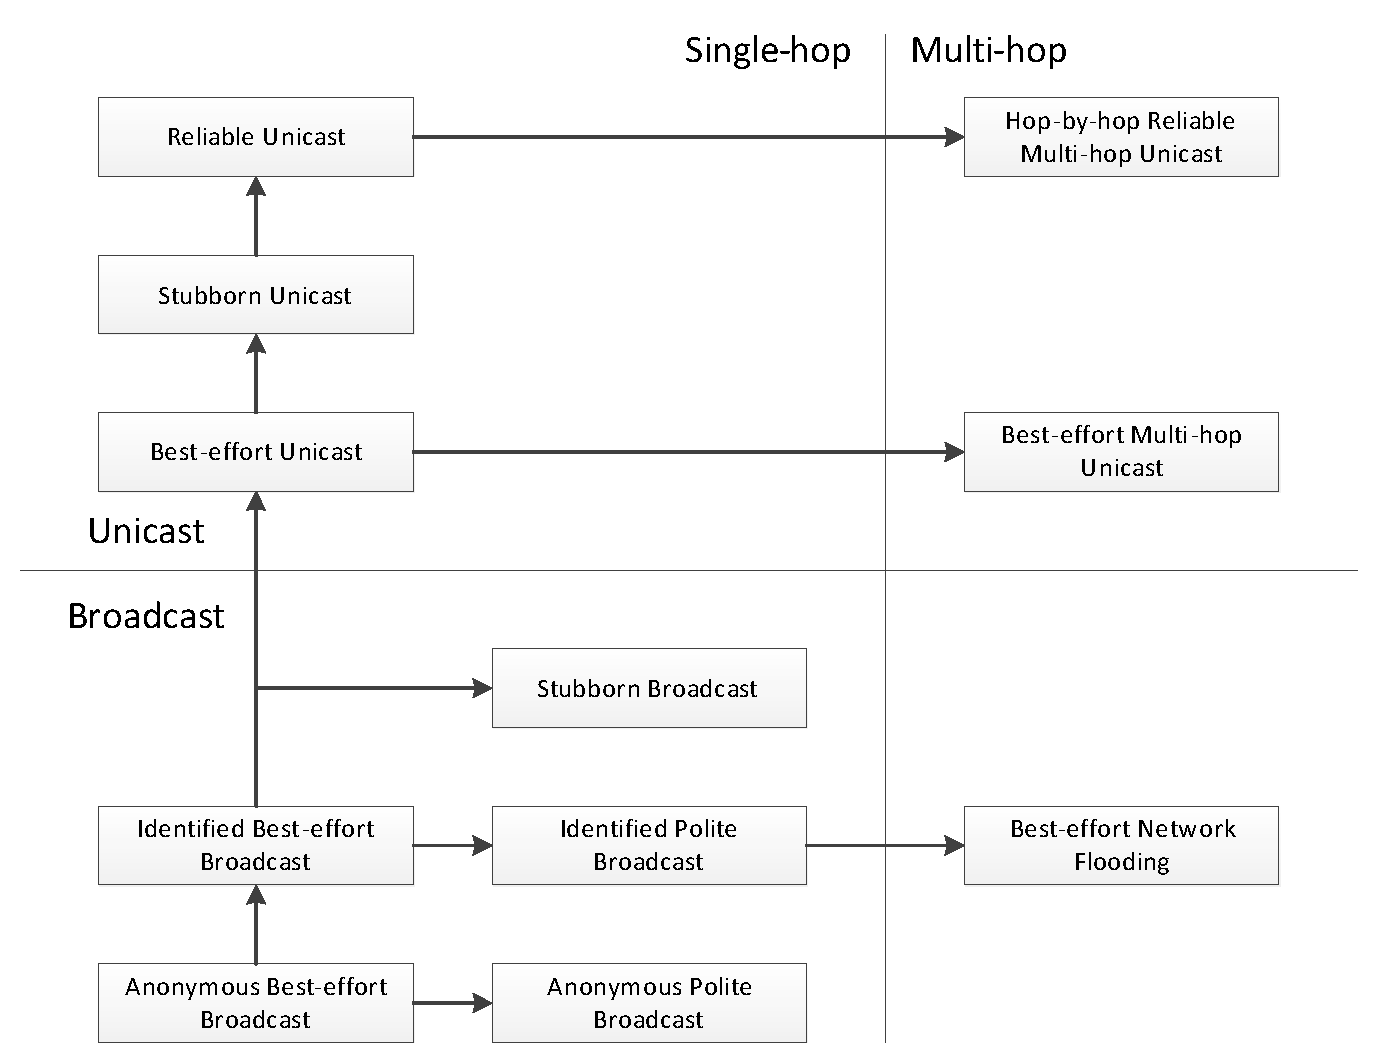
\includegraphics[width=\textwidth]{Diagrams/rime-stack}
	\caption{The communication primitives in the Rime network stack \cite{Dunkels:2007:ACA:1322263.1322295}}
\end{figure}

\begin{table}[H]
	\centering
	\begin{tabular}{ | l | l | l | }
		\hline
		Name & Header & Address \\
		\hline
		Anonymous Broadcast & abc.h & \url{contiki.sourceforge.net/docs/2.6/a01717.html} \\
		Broadcast & broadcast.h & \url{contiki.sourceforge.net/docs/2.6/a01720.html} \\
		Stubborn Broadcast & stbroadcast.h & \url{contiki.sourceforge.net/docs/2.6/a01739.html} \\
		Anonymous Polite Broadcast & polite.h & \url{contiki.sourceforge.net/docs/2.6/a01730.html} \\
		Polite Broadcast & ipolite.h & \url{contiki.sourceforge.net/docs/2.6/a01724.html} \\
		Unicast & unicast.h & \url{contiki.sourceforge.net/docs/2.6/a01738.html} \\
		Stubborn Unicast & stunicast.h & \url{contiki.sourceforge.net/docs/2.6/a01740.html} \\
		Reliable Unicast & runicast.h & \url{contiki.sourceforge.net/docs/2.6/a01738.html} \\
		Network Flooding & netflood.h & \url{contiki.sourceforge.net/docs/2.6/a01728.html} \\
		Multi-hop Unicast & multihop.h & \url{contiki.sourceforge.net/docs/2.6/a01726.html} \\
		Reliable Multi-hop Unicast & rmh.h & \url{contiki.sourceforge.net/docs/2.6/a01732.html} \\
		\hline
		\hline
		Mesh & mesh.h & \url{contiki.sourceforge.net/docs/2.6/a01725.html} \\
		Collect & collect.h & \url{contiki.sourceforge.net/docs/2.6/a01723.html} \\
		Trickle & trickle.h & \url{contiki.sourceforge.net/docs/2.6/a01742.htmll} \\
		\hline
	\end{tabular}
	\caption{Communication Primitives headers and documentation location}
\end{table}


\begin{table}[H]
	\centering
	\begin{tabular}{ | l | l | l | l | }
		\hline
		Name & Reliable & Target & Sender Known\\
		\hline
		Anonymous Broadcast & No & 1-hop neighbours & No\\
		Broadcast & No & 1-hop neighbours & Yes\\
		Stubborn Broadcast & No & 1-hop neighbours & No\\
		Anonymous Polite Broadcast & No & 1-hop neighbours & No\\
		Polite Broadcast & No & 1-hop neighbours & Yes\\
		Unicast & No & destination & Yes\\
		Stubborn Unicast & No & destination & Yes\\
		Reliable Unicast & Yes & destination & Yes\\
		Network Flooding & No & network & Yes\\
		Multi-hop Unicast & No & destination & Yes\\
		Reliable Multi-hop Unicast & Yes & destination & Yes\\
		\hline
		\hline
		Mesh & No & destination & Yes \\
		Collect & Yes & destination & Yes \\
		Trickle & Yes & network & No \\
		\hline
	\end{tabular}
	\caption{Communication Primitives behaviour}
\end{table}

\subsubsection{Anonymous Best-effort Broadcast}

This is the most basic kind of message transmission primitive in Contiki's Rime network stack. It broadcasts a single packet with a maximum length to its 1-hop neighbours. No information about the sender is included within the transmission. It is not usually the case that this type of broadcast is used, as more reliable, more informative primitives (that are built on this one) are often used instead.

\begin{listing}[H]
\begin{minted}[fontsize=\small]{c}
void abc_open(struct abc_conn *c, uint16_t channel, const struct abc_callbacks *u);
void abc_close(struct abc_conn *c);
int abc_send(struct abc_conn *c);

struct abc_callbacks {
   void(* recv)(struct abc_conn *ptr);
};
\end{minted}
\caption{Contiki Anonymous Best-effort Broadcast APIs}
\end{listing}

\subsubsection{Identified Best-effort Broadcast}

This broadcast primitive is essentially the same as the Anonymous Best-effort Broadcast primitive, except for the fact that the address of the sender is included within the header of the message. This address is then made available to the developer when the \verb|recv| callback is called (as can been seen in \autoref{lst:IBEB}).

\begin{listing}[H]
\begin{minted}[fontsize=\small]{c}
void broadcast_open(struct broadcast_conn *c, uint16_t channel,
                    const struct broadcast_callbacks *u);
void broadcast_close(struct broadcast_conn *c);
int broadcast_send(struct broadcast_conn *c);

struct broadcast_callbacks {
   void(* recv)(struct broadcast_conn *ptr, const rimeaddr_t *sender);
};
\end{minted}
\caption{Contiki Identified Best-effort Broadcast APIs}
\label{lst:IBEB}
\end{listing}


\subsubsection{Stubborn Broadcast}

\begin{listing}[H]
\begin{minted}[fontsize=\small]{c}
void stbroadcast_open(struct stbroadcast_conn *c, uint16_t channel,
                      const struct stbroadcast_callbacks *u);
void stbroadcast_close(struct stbroadcast_conn *c);
void stbroadcast_set_timer(struct stbroadcast_conn *c, clock_time_t t);
int stbroadcast_send_stubborn(struct stbroadcast_conn *c, clock_time_t t);
void stbroadcast_cancel(struct stbroadcast_conn *c);

struct stbroadcast_callbacks {
   void (* recv)(struct stbroadcast_conn *c);
   void (* sent)(struct stbroadcast_conn *c);
};
\end{minted}
\caption{Contiki Stubborn Broadcast APIs}
\end{listing}

\subsubsection{Anonymous Polite Broadcast}

\begin{listing}[H]
\begin{minted}[fontsize=\small]{c}
void polite_open(struct polite_conn *c, uint16_t channel,
                 const struct polite_callbacks *cb);
void polite_close(struct polite_conn *c);
int polite_send(struct polite_conn *c, clock_time_t interval, uint8_t hdrsize);
void polite_cancel(struct polite_conn *c);

struct stbroadcast_callbacks {
   void(* recv)(struct polite_conn *c);
   void(* sent)(struct polite_conn *c);
   void(* dropped)(struct polite_conn *c);
};
\end{minted}
\caption{Contiki Anonymous Polite Broadcast APIs}
\end{listing}

\subsubsection{Identified Polite Broadcast}

\begin{listing}[H]
\begin{minted}[fontsize=\small]{c}
void ipolite_open(struct ipolite_conn *c, uint16_t channel,
                  uint8_t maxdups, const struct ipolite_callbacks *cb);
void ipolite_close(struct ipolite_conn *c);
int ipolite_send(struct ipolite_conn *c, clock_time_t interval, uint8_t hdrsize);
void ipolite_cancel(struct ipolite_conn *c);

struct stbroadcast_callbacks {
   void(* recv)(struct ipolite_conn *c, const rimeaddr_t *from)
   void(* sent)(struct ipolite_conn *c);
   void(* dropped)(struct ipolite_conn *c);
};
\end{minted}
\caption{Contiki Identified Polite Broadcast APIs}
\end{listing}

\subsubsection{Best-effort Unicast}

\begin{listing}[H]
\begin{minted}[fontsize=\small]{c}
void unicast_open(struct unicast_conn *c, uint16_t channel, const struct unicast_callbacks *u);
void unicast_close(struct unicast_conn *c);
int unicast_send(struct unicast_conn *c, const rimeaddr_t *receiver);

struct unicast_callbacks {
   void (* recv)(struct unicast_conn *c, const rimeaddr_t *from);
   void (* sent)(struct unicast_conn *ptr, int status, int num_tx);
};
\end{minted}
\caption{Contiki Best-effort Unicast APIs}
\end{listing}

\subsubsection{Stubborn Unicast}

\begin{listing}[H]
\begin{minted}[fontsize=\small]{c}
void stunicast_open(struct stunicast_conn *c, uint16_t channel,
                    const struct stunicast_callbacks *u);
void stunicast_close(struct stunicast_conn *c);
int stunicast_send_stubborn(struct stunicast_conn *c,
                            const rimeaddr_t *receiver, clock_time_t rxmittime);
void stunicast_cancel(struct stunicast_conn *c);
int stunicast_send(struct stunicast_conn *c, const rimeaddr_t *receiver);
void stunicast_set_timer(struct stunicast_conn *c, clock_time_t t);
rimeaddr_t *stunicast_receiver(struct stunicast_conn *c);

struct stunicast_callbacks {
   void (* recv)(struct stunicast_conn *c, const rimeaddr_t *from);
   void (* sent)(struct stunicast_conn *c, int status, int num_tx);
};
\end{minted}
\caption{Contiki Stubborn Unicast APIs}
\end{listing}

This is in fact anonymous, it will not send the address of the node that send the message in the header of the message. If a node needs to know who sent the message, then the sender's address should be included in the body.


\subsubsection{Reliable Unicast}

\begin{listing}[H]
\begin{minted}[fontsize=\small]{c}
void runicast_open(struct runicast_conn *c, uint16_t channel,
                   const struct runicast_callbacks *u);
int runicast_send(struct runicast_conn *c, const rimeaddr_t *receiver,
                  uint8_t max_retransmissions);
uint8_t runicast_is_transmitting(struct runicast_conn *c);

struct runicast_callbacks {
   void (* recv)(struct runicast_conn *c, const rimeaddr_t *from, uint8_t seqno);\cite{
   void (* sent)(struct runicast_conn *c, const rimeaddr_t *to, uint8_t retransmissions);
   void (* timedout)(struct runicast_conn *c, const rimeaddr_t *to, uint8_t retransmissions);
};
\end{minted}
\caption{Contiki Reliable Unicast APIs}
\end{listing}

\subsubsection{Best-effort Network Flooding}

\begin{listing}[H]
\begin{minted}[fontsize=\small]{c}
void netflood_open(struct netflood_conn *c, clock_time_t queue_time,
                   uint16_t channel, const struct netflood_callbacks *u);
void netflood_close(struct netflood_conn *c);
int netflood_send(struct netflood_conn *c, uint8_t seqno);

struct netflood_callbacks {
   int (* recv)(struct netflood_conn *c, const rimeaddr_t *from,
                const rimeaddr_t *originator, uint8_t seqno, uint8_t hops);
   void (* sent)(struct netflood_conn *c);
   void (* dropped)(struct netflood_conn *c);
};
\end{minted}
\caption{Contiki Best-effort Network Flooding APIs}
\end{listing}

\subsubsection{Best-effort Multi-hop Unicast}

\begin{listing}[H]
\begin{minted}[fontsize=\small]{c}
void rmh_open(struct rmh_conn *c, uint16_t channel, const struct rmh_callbacks *u);
void rmh_close(struct rmh_conn *c);
int rmh_send(struct rmh_conn *c, rimeaddr_t *to, uint8_t num_rexmit, uint8_t max_hops);

struct rmh_callbacks {
   void (* recv)(struct rmh_conn *ptr, rimeaddr_t *sender, uint8_t hops);
   rimeaddr_t *(* forward)(struct rmh_conn *ptr,
                          const rimeaddr_t *originator,
                          const rimeaddr_t *dest,
                          const rimeaddr_t *prevhop,
                          uint8_t hops);
};
\end{minted}
\caption{Contiki Best-effort Multi-hop Unicast APIs}
\end{listing}

\subsubsection{Hop-by-hop Reliable Multi-hop Unicast}

\begin{listing}[H]
\begin{minted}[fontsize=\small]{c}
void multihop_open(struct multihop_conn *c, uint16_t channel,
                   const struct multihop_callbacks *u);
void multihop_close(struct multihop_conn *c);
int multihop_send(struct multihop_conn *c, const rimeaddr_t *to);
void multihop_resend(struct multihop_conn *c, const rimeaddr_t *nexthop);

struct multihop_callbacks {
   void (* recv)(struct multihop_conn *ptr,
                 const rimeaddr_t *sender,
                 const rimeaddr_t *prevhop,
                 uint8_t hops);
   rimeaddr_t *(* forward)(struct multihop_conn *ptr,
                           const rimeaddr_t *originator,
                           const rimeaddr_t *dest,
                           const rimeaddr_t *prevhop,
                           uint8_t hops);
};
\end{minted}
\caption{Contiki Hop-by-hop Reliable Multi-hop Unicast APIs}
\end{listing}


\subsection{Mesh Network Protocol}

\begin{listing}[H]
\begin{minted}[fontsize=\small]{c}
void mesh_open(struct mesh_conn *c, uint16_t channels, const struct mesh_callbacks *callbacks);
void mesh_close(struct mesh_conn *c);
int mesh_send(struct mesh_conn *c, const rimeaddr_t *dest);

struct mesh_callbacks {
   /** Called when a packet is received. */
   void (* recv)(struct mesh_conn *c, const rimeaddr_t *from, uint8_t hops);
   /** Called when a packet, sent with mesh_send(), is actually transmitted. */
   void (* sent)(struct mesh_conn *c);
   /** Called when a packet, sent with mesh_send(), times out and is dropped. */
   void (* timedout)(struct mesh_conn *c);
};
\end{minted}
\caption{Contiki Mesh Network APIs}
\end{listing}


\subsection{Collect Network Protocol}

\begin{listing}[H]
\begin{minted}[fontsize=\small]{c}
void collect_open(struct collect_conn *c,
                  uint16_t channels, uint8_t is_router,
                  const struct collect_callbacks *callbacks);
void collect_close(struct collect_conn *c);
int collect_send(struct collect_conn *c, int rexmits);
void collect_set_sink(struct collect_conn *c, int should_be_sink);
int collect_depth(struct collect_conn *c);
const rimeaddr_t *collect_parent(struct collect_conn *c);
void collect_set_keepalive(struct collect_conn *c, clock_time_t period);

struct collect_callbacks {
   void (* recv)(const rimeaddr_t *originator, uint8_t seqno,
                 uint8_t hops);
};
\end{minted}
\caption{Contiki Collect Network APIs}
\end{listing}


\subsection{Trickle Network Protocol}

\begin{listing}[H]
\begin{minted}[fontsize=\small]{c}
void trickle_open(struct trickle_conn *c, clock_time_t interval,
                  uint16_t channel,
                  const struct trickle_callbacks *cb);
void trickle_close(struct trickle_conn *c);
void trickle_send(struct trickle_conn *c);

struct trickle_callbacks {
   void (* recv)(struct trickle_conn *c);
};
\end{minted}
\caption{Contiki Trickle Network APIs}
\end{listing}


\subsection{Network Channels}

Channels in Contiki are virtual \cite{tel-aviv-contiki-exercises, Dunkels:2007:ACA:1322263.1322295}. This means that when a connection is opened if you do not want to receive packets from another connection then a different channel should be used. It does not mean that different radio frequencies are used. To use different radio frequencies the function \verb|cc2420_set_channel| should be used to change the frequency messages are broadcasted on.


\subsection{Timers}

\subsubsection{Event Timer}

\url{http://contiki.sourceforge.net/docs/2.6/a01667.html}

\subsubsection{Callback Timer}

\url{http://contiki.sourceforge.net/docs/2.6/a01666.html}

\clearpage

% !TeX root = Report.tex
\section{Implemented Algorithms}

\dirtree{%
.1 Common/.
.2 containers/.
.3 linked-list.[h/c].
.3 array-list.[h/c].
.3 unique-array.[h/c].
.3 map.[h/c].
.2 net/.
.3 eventupdate.[h/c].
.3 multipacket.[h/c].
.3 nhopflood.[h/c].
.3 nhopreq.[h/c].
.3 rimeaddr-helpers.[h/c].
.3 tree-aggregator.[h/c].
.2 debug-helper.[h/c].
.2 led-helper.[h/c].
.2 random-range.[h/c].
.2 sensor-converter.[h/c].
}

\subsection{Container Library}

Contiki comes with a list container \footnote{Header: \url{https://github.com/contiki-os/contiki/blob/master/core/lib/list.h} Source: \url{https://github.com/contiki-os/contiki/blob/master/core/lib/list.c}}, however, when we were developing with their linked list we found that it was awkward to use in some situations (for instance creating an array of lists) so we decided that we needed to find a better list library. Our problem was that other container libraries were unlikely to be optimised to the low memory requirements or support the special compile chain used by Contiki. So rather than waste time searching and integrating an external library we decided to write our own set of containers. By doing the main benefit we gained was that we knew how the containers worked so had a better understanding how to use them.

Another reason to develop our own containers was that we desired an list where the data was stored in an array, this was for because it provides lower memory overhead and the types of operations we would be performing (append and empty) meant that an array backed list would be better. The lower memory overhead comes from the fact that an array-based list doesn't need to store a pointer to the next element as it is implicit (due to the contiguous memory) that a pointer to the current element's pointer plus one is the next element. This means that in a list of $N$ items our singly linked list implementation will require $(\text{sizeof}(T) + \text{sizeof}(void *) \times 2) \times N$ bytes of memory, whereas our array list implementation will require $(\text{sizeof}(T) + \text{sizeof}(void *)) \times N$ bytes of memory.

Our linked list implementation uses more memory compared to Contiki's implementation because their list is \emph{intrusive}\footnote{Boost Containers: \url{http://www.boost.org/doc/libs/1\_53\_0/doc/html/intrusive/presenting\_containers.html}}. What is meant by this is that the pointer to the next item in the list is contained in the structure stored in the list \cite{?}. Meaning their list uses the same amount of memory as our array list. However, because the list is intrusive it makes it more difficult to use as the implementation detail leaks into the structure using the library, this was why developing our own non-intrusive list made it easier to develop code.

We also developed containers that helped abstract certain concepts (such as list uniqueness or accessing elements by key) to decrease code duplication and allow us to express the code in a higher-level way making implementation easier. One thing to note is that for the containers we did not focus on implementing some of their functions to the standard complexity. For example our map implementation has requires O(N) for both insert and fetching, where these may be implemented as O(1) on average (hash tables) or O(log N) (trees), however due to the requirements of low memory we decided to keep using the array as the backing store for the data with the aim to keep memory for at the expense of non-optimal container management functions. The increased time complexity should make little difference as the containers tend to have few elements in them (i.e. hundreds rather than millions, where complexity would start to be important \cite{?}).

Finally, all of these custom containers are tested by a test suite that checks for functional correctness. Also the test suite was run using \verb|valgrind|\footnote{\url{http://valgrind.org/info/tools.html}} to check for memory leaks and corruption.

\subsection{Network Library}

\subsubsection{Event Update}

\begin{figure}[H]
  \centering
  \begin{boxedminipage}{\linewidth}
    % 
    \null Process $j$ - \res{event-update}\\
    %
    \null \textbf{variables}\\
    %
    \null\qq \var{period}: timer init $P_{generate}$;\\~\\
    %
    \null\qq \% The previous node data sent to the network\\
    \null\qq \var{previous}: struct init $\bot$;\\~\\
    %
    \null \textbf{constants}\\
    %
    \null\qq \% Generate Period, how often we should check for a change in the data\\
    \null\qq \var{$P_{generate}$}: time;\\~\\
    %
    \null\qq \% Checks if the data differs\\
    \null\qq \var{differs}: function takes (struct, struct) returns boolean;\\~\\
    %
    \null\qq \% Gets the data of the current node\\
    \null\qq \var{data}: function takes () returns struct;\\~\\
    %
    \null\qq \% The probability of sending our data, even if no change occurred\\
    \null\qq \var{chance}: real;\\~\\
    %
    \null \textbf{parameters}\\
    %
    \null\qq \% The distance we need to send information\\
    \null\qq \var{distance}: int;\\~\\
    %
    \null \textbf{actions}\\
    %
    %
    \null\qq \% Check for changes\\
    \null\qq \emph{check}::~\res{timeout}(\var{period}) $\rightarrow$\\
    \null\qq\qq $\var{force} \assign \res{RandReal}(0, 1) \leq \var{chance}$;\\
    \null\qq\qq $\var{changed} \assign \var{previous} = \bot \lor \var{differs}(\var{data}(), \var{previous})$;\\
    \null\qq\qq \res{if} ($\var{force} \lor \var{changed}$) \res{then}\\
    \null\qq\qq\qq $\var{previous} \assign \var{data}()$;\\
    \null\qq\qq\qq \res{nhopflood}$\langle j, \var{previous}, \var{distance}\rangle$;\\
    \null\qq\qq \res{fi}; \\
    \null\qq\qq \res{set}($\mathit{period}$, $P_{generate}$); \\~\\
    %
    %
    \null\qq \% Receiving Change message\\
    \null\qq \emph{receive}::~\res{nhopflood.recv}$\langle source, data, hops\rangle \rightarrow$\\
    \null\qq\qq \% Prevent delivery if being told that the current node's data has changed\\
    \null\qq\qq \res{if} ($j \not= source$) \res{then} \\
    \null\qq\qq\qq \% Inform library caller of data change\\
    \null\qq\qq\qq \res{data-changed-callback}(\var{data}, \var{hops}); \\
    \null\qq\qq \res{fi}; \\
    %
    %
  \end{boxedminipage}
  \caption{Event Update Broadcast Algorithm}
\end{figure}


\subsubsection{Multi-Packet}

In Contiki sending a single packet has its limits, there is only so much data you can get in a single packet. There are two C macros that are relevant to this \verb|PACKETBUF_HDR_SIZE| which is set to 48 bytes and \verb|PACKETBUF_SIZE| which is set to 128 bytes\footnote{packetbuf.h \url{http://contiki.sourceforge.net/docs/2.6/a00302.html}}. This means that in general we will only be able to send a packet containing 128 bytes of information, but what if we have a data structure that spans 300 bytes? Then we will need to have a way to send multiple packets and a receiver that can put the packets back together in the correct way to deliver the data.

Contiki's data transfer primitives for their RIME protocols are fairly hidden because of their focus on uIPv6. We found \verb|ruldolph0| first \footnote{ruldolph0 \url{http://contiki.sourceforge.net/docs/2.6/a01735.html}} and then \verb|rucb| (Reliable Unicast Bulk Transfer) much later \footnote{rucb \url{http://contiki.sourceforge.net/docs/2.6/a00365.html}}. However, both of them have problems, the API is very convoluted and seems more geared towards sending very large files across the network. This is very different to our aim, which is to send relatively small packets of data to a specific neighbour. So we wrote our own API that would split data of any given size and reassemble it once received, our API was not focused on processing data chunks like \verb|ruldolph0| or \verb|rucb|, but simply operated on a block of memory given to it. This is a case where a simpler API made development much easier for us. Admittedly because our implementation uses dynamic memory allocation it could potentially perform worse, but because the energy of sending and receiving messages dwarfs the energy usage of the CPU, we feel that easier development tradeoff made it worth it. Also, now that code has been written to use this API, the \verb|multipacket| library itself could always be rewritten to use \verb|rucb| as a base to run more efficiently.

\subsubsection{N-Hop Request} 

We developed the N-Hop Request communication layer very early in the project. Our application needed a way to pass predicate messages between nodes, these messages sometimes needed to travel multiple hops in the network and also contain routing information for the receiving node, so that it could respond to the originator. Firstly, we consulted the Contiki libraries to see if any of the existing network primitives could be used for this purpose. We initially considered \verb|Mesh| which sends a packet to any node on the network, this seemed like it would be a prefect fit for sending data back to the originator node; However, issues arose when we discovered that it could only send one unique packet across the network at a time. This was due to the way that \verb|Mesh| was implemented, it only maintains a record of the most recently received packet on the network. This assumption is fine if you assume that you only have 1 sender like a base station but when you have multiple senders sending different packets it fails. Next we considered \verb|Trickle| \footnote{trickle.h \url{http://contiki.sourceforge.net/docs/2.6/a00381.html}}. Unfortunately, like \verb|Mesh|, \verb|Trickle| had similar short comings which made unsuitable for our task. In some cases \verb|reliable unicast| could be used to target the specific nodes for which the message is intended. This, however, is not suitable when the identifies of the nodes is not known, or in situations when storing routing tables is not appropriate. 

Having explored several options from the Contiki source library we realised that N-Hop Request had a very specific set of requirements. We found that no one library offered all the functionality we needed; Therefore, We opted for developing our own communication layer and API to handle the routing of these messages. The layer would need to flood the network, a fixed number of hops from the source, whilst allowing multiple nodes to use the same layer, with different messages. For this we used existing Contiki Rime Protocol implementations and initially the primitive was heavily influenced by the H-Send\cite{HSEND} algorithm, we started by implementing a variation of H-Send which we then went onto generalise for predicates that could be defined at run-time by our GUI running on the base station.

The libraries that we used were \verb|stbroadcast| (Stubborn Broadcast) and \verb|runicast| (Reliable Unicast). Stubborn Broadcast is used by the originator to send the request for application and network information n-hops in the network. Every node that receives the request checks the hop count in the message; if it's $\> 1$ then, it decrements the hop count and forwards the packet on to it's neighbours using Stubborn Broadcast. Every node that receives this request then waits a random amount of time with it's rime address as a seed and then uses Reliable Unicast to send it's application and Network Information back to the node it received the request from. If a node receives this packet and isn't the intended target (the originator) they forward packet on to the node that they received their request message from, eventually the packet will arrive back at the originator who can then deliver the message. In order to minimise message sends, each node maintains the most efficient node to get back to the originator. This is based on the number of hops it takes for a request message to reach the node, a message from a node with 3 hops left is a more efficient route than a message from a node with only 2 hops left. Finally, once a pre-determined wait period has expired the gathered data is passed to the predicate evaluator and any further data received is not delivered.

%TODO: Note about performance maybe?
%Could also put a graphic of the chain here too

\begin{figure}[H]
  \centering
  \begin{boxedminipage}{\linewidth}
    % 
    \null Process $j$ - \verb|n-hop-req|\\
    %
    \null \textbf{parameters}\\
    %
    \null\qq \% The number of hops left to send a message\\
    \null\qq \var{hop\_limit}: int\\~\\
    %
    %
    \null \textbf{variables}\\
    %
    \null\qq \%The nodes a given message was seen from\\
    \null\qq \var{mote\_records}: map\\~\\
    %
    %
    \null \textbf{constants}\\
    %
    \null\qq \% Send Data Period, the time between receiving a request for data, and sending it\\
    \null\qq \var{$P_{send\_data}$}: time;\\~\\
    %
    %
    \null \textbf{actions}\\
    %
    %
    \null\qq \% Receiving Message\\
    \null\qq \emph{receive}::~\res{recv}$\langle source, data, hop\_count, id\rangle \rightarrow$\\
    \null\qq\qq \res{if} ($mote\_records.contains(id)$) \res{then}\\
    \null\qq\qq\qq \res{if} ($mote\_records.hop\_count(id) < hop\_count$) \res{then} \\
    \null\qq\qq\qq\qq \res{stbroadcast.send($message$,$hop\_count -1$)};\\
    \null\qq\qq\qq\qq \res{$mote\_records$.replace($id$,$hop\_count$)};\\
    \null\qq\qq\qq\qq \res{\var{$P_{send\_data}$}.restart()}\\
    \null\qq\qq\qq \res{fi;}\\
    \null\qq\qq \res{else}\\
    \null\qq\qq\qq \res{stbroadcast.send($message$,$hop\_count -1$)};\\
    \null\qq\qq\qq \res{$mote\_records$.add($id$,$data$,$source$,$hop\_count$)};\\
    \null\qq\qq\qq \res{\var{$P_{send\_data}$}.start()}\\
    \null\qq\qq \res{fi;}\\~\\
    %
    %
    \null\qq \% Sending Data\\
    \null\qq \emph{send\_data}:~\res{timeout}(\var{$P_{send\_data}$})$\rightarrow$\\
    \null\qq\qq \res{runicast.send}($j$,$mote\_records.getMote(id)$, $data$);\\~\\
    %
    %
    \null\qq \% Recieved Data\\
    \null\qq \emph{recv\_data}:~\res{runicast.recv}$\langle source, data, id\rangle \rightarrow$\\
    \null\qq\qq \res{if} ($mote\_records.getMote(id)$ == $self$) \res{then}\\
    \null\qq\qq\qq \% Process Data\\
    \null\qq\qq \res{else}\\
    \null\qq\qq\qq \res{runicast.send}($mote\_records.getMote(id)$, $data$);\\
    \null\qq\qq \res{fi;}\\
    %
    %
  \end{boxedminipage}
  \caption{N-Hop Request Algorithm}
  \label{fig:n-hop-req-algorithm}
\end{figure}

\subsubsection{N-Hop Flood}

To improve upon the efficiency of our initial implementation of N-Hop Request we decide to implement a separate protocol for situations where every node in the network is evaluating the same predicate. Firstly we considered the problem, in this situation we know that every node requires the application and network information of every other node in it's N-Hop radius (determined by the predicate being evaluated). Since every node is evaluating the predicate and all nodes know that, we can forgo the request phase of the N-Hop Request implementation; Instead, we simply flood our N-Hop neighbours with our application and network data and the other nodes in the network do the same. 

The N-Hop Flood protocol uses the Rime \verb|broadcast| primitive to send all it's messages to neighbouring nodes. It maintains a buffer of all the packets received and is provided with parameters on initialisation to determine how long each broadcasting round is and how often the protocol must re-broadcast messages within the round. Every node in the network continues to rebroadcast it's own message as well as any packets in the buffer if they have a hop count of $\> 1$, this occurs every time the rebroadcast interval completes. Once the round is finished the message buffer is cleared and all timers are reset.

\begin{figure}[H]
  \centering
  \begin{boxedminipage}{\linewidth}
    % 
    \null Process $j$ - \verb|n-hop-flood|\\
    %
    \null \textbf{parameters}\\
    %
    \null\qq \% The number of hops left to send a message\\
    \null\qq \var{hop\_limit}: int\\~\\
    %
    \null\qq \% The send period for this predicate\\
    \null\qq \var{send\_period}: time\\~\\
    %
    \null\qq \% The max number of times to re-transmit\\
    \null\qq \var{maxrx}: int\\~\\
    %
    %
    \null \textbf{variables}\\
    %
    \null\qq \% The queue of packets that need to be broadcast\\
    \null\qq \var{packet\_queue}: linked list\\~\\
    %
    \null\qq \% The map of all messages received from the nodes N-Hop neighbours\\
    \null\qq \var{latest\_message\_seen}: map\\~\\
    %
    %
    \null \textbf{actions}\\
    %
    %
    \null\qq \% Broadcast Data\\
    TODO...
    %
    %
    \null\qq \% Recieved Data\\
    \null\qq \emph{recv\_data}:~$\langle data, sender\rangle \rightarrow$\\
    \null\qq\qq \res{if} ($latest\_message\_seen.getMessage(sender)$ == $NULL$) \res{then}\\
    \null\qq\qq\qq \% \res{latest\_message\_seen.addMessage}($sender$, $data$);\\
    \null\qq\qq \res{else}\\
    \null\qq\qq\qq Ignore the Data\\
    \null\qq\qq \res{fi;}\\
    %
    %
  \end{boxedminipage}
  \caption{N-Hop Flood Algorithm}
  \label{fig:n-hop-flood-algorithm}
\end{figure}

\subsubsection{Neighbour Detection}

\subsubsection{Tree Aggregation}

As has been previously mentioned Tree Aggregation is a very useful technique employed in wireless sensor networks to aggregate a set of data to a single node in the network. It is very useful because of its ability to convey the same amount of data in potentially fewer messages. The algorithm works by first creating a tree structure such that nodes know of a parent node that they should unicast their messages to. Once this tree is set up the nodes (typically leaf nodes) unicast data to their parents, this can either happen when an event occurs or it can happen periodically. When a parent node receives a message it waits for a certain amount of time for more messages to arrive, every message it receives is stored and aggregated. After the time period is up the aggregated data is forwarded to its parent node. Once the data reaches the destination it is delivered to the user of the library.


The user of this library needs to implement four important functions:
\begin{enumerate}
\item[$\otimes_{agg}$] This function aggregates stored data with data message that has been received
\item[$\otimes_{own}$] This function aggregates the node's own data into the stored data
\item[$\otimes_{read}$] This function does the initial reading of data from a message and creates the local stored data
\item[$\otimes_{write}$] This function writes the local stored data back to a packet
\end{enumerate}


\begin{figure}[H]
  \centering
  \begin{boxedminipage}{\linewidth}
    % 
    \null Process $j$ - \res{tree-aggregation}\\
    %
    \null \textbf{variables}\\
    %
    \null\qq \var{parentdetect}: timer init $\bot$;\\~\\
    %
    \null\qq \var{seensetup}, \var{collecting}, \var{leaf}: bool init $False$, $False$, $True$;\\~\\
    %
    \null\qq \var{besthop}: int init $INTMAX$;\\~\\
    %
    \null\qq \var{bestparent}: address init $\bot$;\\~\\~\\
    %
    \null\qq \var{aggregation}: timer init $\bot$;\\~\\
    %
    \null\qq \var{collecting}: bool init $False$;\\~\\
    %
    \null\qq \var{stored}: struct init $\bot$;\\~\\
    %
    \null \textbf{constants}\\
    %
    \null\qq \% How long to wait for messages to aggregate before forwarding what the node has\\
    \null\qq \var{$P_{aggregation}$}: time;\\~\\
    %
    \null\qq \% How long to wait for parents to be detected\\
    \null\qq \var{$P_{parentdetect}$}: time;\\~\\
    %
    \null \textbf{parameters}\\
    %
    \null\qq \% The address of the node data should be aggregated to\\
    \null\qq \var{sink}: address;\\
    %
  \end{boxedminipage}
  \caption{Tree Aggregation Algorithm - variables}
\end{figure}

\begin{figure}[H]
  \centering
  \begin{boxedminipage}{\linewidth}
    \null \textbf{actions}\\
    %
    %
    \null\qq \% Set up tree: initialise\\
    \null\qq \emph{starup}::~\res{init} $\rightarrow$\\
    \null\qq\qq \res{bcast}$\langle j, \bot, 1\rangle$;\\~\\
    %
    %
    \null\qq \% Set up tree: receive message\\
    \null\qq \emph{receive}::~\res{recv}$\langle source, parent, hops\rangle \rightarrow$\\
    \null\qq\qq \res{if} ($j \not= sink$) \res{then} \\
    \null\qq\qq\qq \res{if} ($\lnot\var{seensetup}$) \res{then} \\
    \null\qq\qq\qq\qq $\var{seensetup} \assign True$; \\
    \null\qq\qq\qq\qq \res{set}($\mathit{parentdetect}$, $P_{parentdetect}$); \\
    \null\qq\qq\qq \res{fi}; \\
    \null\qq\qq\qq \res{if} ($\var{hops} < \var{besthop}$) \res{then} \\
    \null\qq\qq\qq\qq $\var{bestparent}, \var{besthop} \assign \var{source}, \var{hops}$; \\
    \null\qq\qq\qq \res{fi}; \\
    \null\qq\qq\qq \res{if} ($\var{leaf} \land \var{j} = \var{parent}$) \res{then} \\
    \null\qq\qq\qq\qq $\var{leaf} \assign False$; \\
    \null\qq\qq\qq \res{fi}; \\
    \null\qq\qq \res{fi}; \\~\\
    %
    %
    \null\qq \% Set up tree: finish detecting parents\\
    \null\qq \emph{check}::~\res{timeout}(\var{parentdetect}) $\rightarrow$\\
    \null\qq\qq \res{if} ($\var{besthop} = INTMAX$) \res{then} \\
    \null\qq\qq\qq \res{bcast}$\langle j, \var{bestparent}, INTMAX\rangle$;\\
    \null\qq\qq \res{else} \\
    \null\qq\qq\qq \res{bcast}$\langle j, \var{bestparent}, \var{besthop} + 1\rangle$;\\
    \null\qq\qq \res{fi}; \\
    %
    %
  \end{boxedminipage}
  \caption{Tree Aggregation Algorithm - Setting up tree}
\end{figure}


\begin{figure}[H]
  \centering
  \begin{boxedminipage}{\linewidth}
    \null \textbf{actions}\\
    %
    %
    \null\qq \% Send data function\\
    \null\qq \emph{send}::~\res{function}$\langle data\rangle \rightarrow$\\
    \null\qq\qq \res{multipacket.unicast}$\langle \var{bestparent}, data\rangle$;\\~\\
    %
    %
    \null\qq \% Set up tree: receive message\\
    \null\qq \emph{receive}::~\res{multipacket.recv}$\langle source, data\rangle \rightarrow$\\
    \null\qq\qq \res{if} ($j = sink$) \res{then} \\
    \null\qq\qq\qq $\var{stored} \assign \otimes_{read}(data)$; \\
    \null\qq\qq\qq $\var{stored} \assign \otimes_{own}(\var{stored})$; \\
    \null\qq\qq\qq $\res{deliver}(\otimes_{write}(\var{stored}))$; \\
    \null\qq\qq \res{else} \\
    \null\qq\qq\qq \res{if} ($\var{collecting}$) \res{then} \\
    \null\qq\qq\qq\qq $\var{stored} \assign \otimes_{agg}(\var{stored}, \var{data})$; \\
    \null\qq\qq\qq \res{else} \\
    \null\qq\qq\qq\qq $\var{stored} \assign \otimes_{read}(data)$; \\
    \null\qq\qq\qq\qq $\var{collecting} \assign True$; \\
    \null\qq\qq\qq\qq \res{set}($\mathit{aggregation}$, $P_{aggregation}$); \\
    \null\qq\qq\qq \res{fi}; \\
    \null\qq\qq \res{fi}; \\~\\
    %
    %
    \null\qq \% Set up tree: finish detecting parents\\
    \null\qq \emph{finishagg}::~\res{timeout}(\var{aggregation}) $\rightarrow$\\
    \null\qq\qq \res{multipacket.unicast}$\langle \var{bestparent}, \otimes_{write}(\var{stored})\rangle$;\\
    \null\qq\qq $\var{collecting} \assign False$; \\
    \null\qq\qq $\var{stored} \assign \bot$; \\
    %
    %
  \end{boxedminipage}
  \caption{Tree Aggregation Algorithm - Sending data}
\end{figure}

\begin{figure}[ht!]
\centering
\subfigure[Example Network]{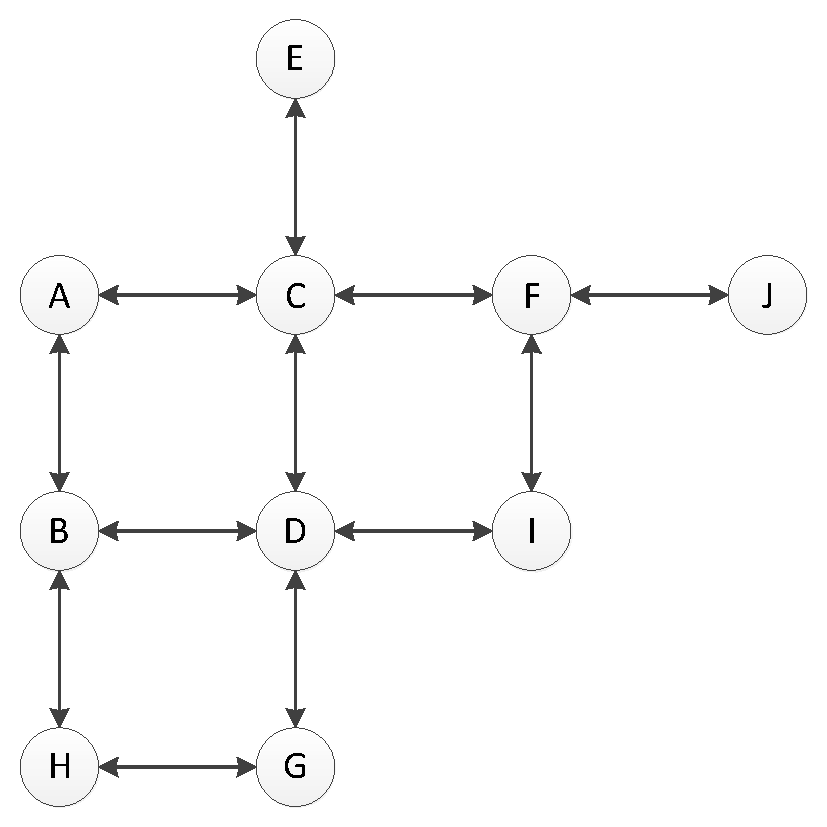
\includegraphics[width=0.5\textwidth]{Diagrams/neighbour-network}}

\subfigure[Logical Tree imposed on network]{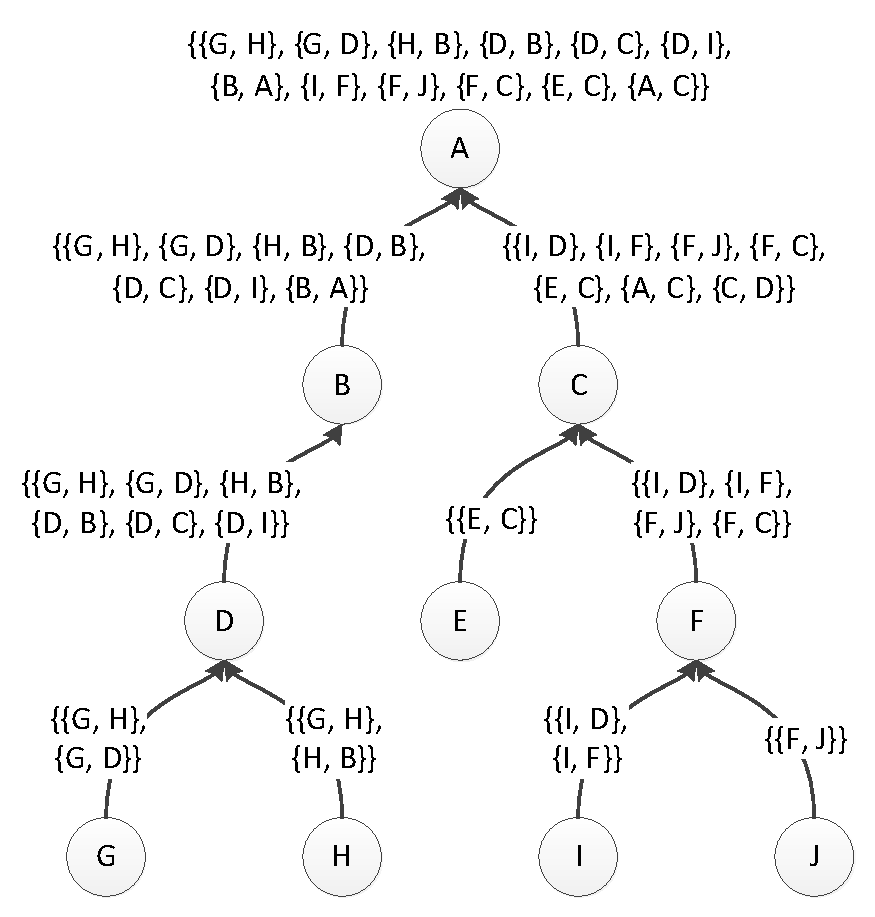
\includegraphics[width=0.5\textwidth]{Diagrams/neighbour-tree-structure}}
\end{figure}

\subsubsection{Neighbour Detect}

To aid in debugging a vital piece of information that will be required about the network is its topology. Trying to analyse network state without knowing which nodes are neighbours of other nodes, makes drawing meaningful conclusions from that data much harder. This meant that we needed a way to send neighbour information back to the sink. Thankfully part of the job is already accomplished as Contiki comes with a library to perform neighbour detection\cite{?}. We extended that library in two ways.

The first was to add more features to Contiki's neighbour detect library. As that library was very simple and supported only saying that a neighbour had been detected (with the option of providing a integer value as well). As we were aiming for this code to support changes in the network, such as nodes leaving or joining neighbourhoods, we added the concept of a round. Instead of just knowing about neighbours at that instant in time, it allowed the library to maintain some kind of history about what nodes were neighbours of other nodes in the past. Whenever new nodes are detected they are recorded, however, if a node has not been detected for a certain number of rounds then that node is removed from the record.

\begin{figure}[ht!]
\centering
\subfigure[Node A requesting neighbour data]{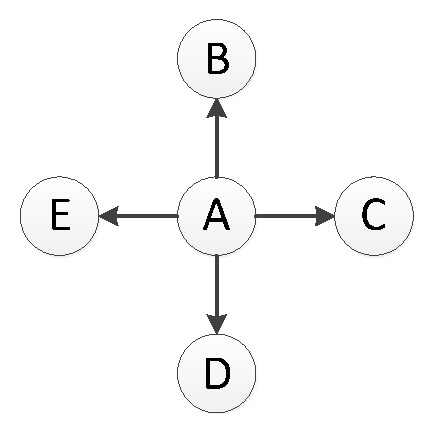
\includegraphics[width=0.25\textwidth]{Diagrams/neighbour-request}}
\subfigure[Node A receiving neighbour data]{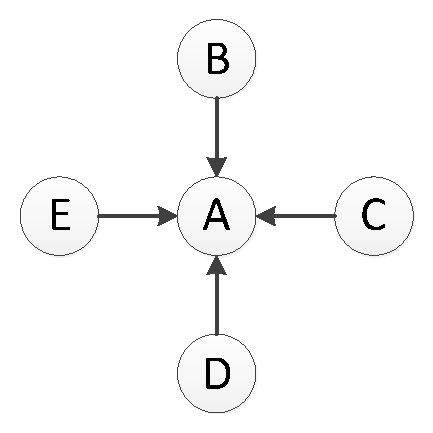
\includegraphics[width=0.25\textwidth]{Diagrams/neighbour-report}}
\caption{Nodes asking for and receiving neighbour data}
\end{figure}

\begin{figure}[H]
  \centering
  \begin{boxedminipage}{\linewidth}
    % 
    \null Process $j$ - \res{neighbourdetect}\\
    %
    \null \textbf{variables}\\
    %
    \null\qq \var{period}: timer init $P_{round}$;\\~\\
    %
    \null\qq \% The history of node\\
    \null\qq \var{previous}: map of address to int init $\emptyset$;\\~\\
    %
    \null\qq \% The current round\\
    \null\qq \var{count}: int init 0;\\~\\
    %
    \null \textbf{constants}\\
    %
    \null\qq \% Round Period\\
    \null\qq \var{$P_{round}$}: time;\\~\\
    %
    \null\qq \% The missed round threshold\\
    \null\qq \var{missed}: int;\\~\\
    %
    \null \textbf{actions}\\
    %
    %
    \null\qq \% Check for changes\\
    \null\qq \emph{round}::~\res{timeout}(\var{period}) $\rightarrow$\\
    \null\qq\qq $\var{previous} \assign \{ (addr, round) \in \var{previous} | count - round \geq missed \}$;\\
    \null\qq\qq \% Tell library caller that a round is finished\\
    \null\qq\qq \res{round-complete}(\res{values}(previous), \var{count});\\
    \null\qq\qq $\var{count} \assign \var{count} + 1$; \\
    \null\qq\qq \res{set}($\mathit{period}$, $P_{round}$); \\~\\
    %
    %
    \null\qq \% Receiving Neighbour Discovery message\\
    \null\qq \emph{neighbour}::~\res{neighbour\_discovery.recv}$\langle source, round\rangle \rightarrow$\\
    \null\qq\qq \% Update the round we last saw this node\\
    \null\qq\qq \res{if} ($source \in \res{keys}(\var{previous})$) \res{then} \\
    \null\qq\qq\qq \res{if} ($round > \var{previous}[\var{source}]$) \res{then} \\
    \null\qq\qq\qq\qq $\var{previous}[\var{source}] \assign \var{round}$; \\
    \null\qq\qq\qq \res{fi}; \\
    \null\qq\qq \res{else} \\
    \null\qq\qq\qq $\var{previous}[\var{source}] \assign \var{round}$; \\
    \null\qq\qq \res{fi}; \\~\\
    %
    %
  \end{boxedminipage}
  \caption{Neighbour Detect Algorithm}
  \label{algo:neighbour-detect}
\end{figure}

For this to be useful we needed a way to get this data back to the sink node. There are many ways to do this, but one of the best is aggregating along a tree because it can combine many messages into a single one and forward that aggregated message instead of lots of smaller messages \cite{?}. The Neighbour Aggregation part uses the Tree Aggregation library that we have developed, the function that is used to aggregate data together is $\cup$ (union), this allows data to be aggregated with other data and allows that data to be updated. The nodes own data is set to be $\res{node-data}$, where $\var{j}$ is the current node's address and $\res{round-data}$ is the set of node addresses provided by the $\res{round-complete}$ callback in \autoref{algo:neighbour-detect}.

\begin{equation}
\res{node-data} = \{\{\var{other}, \var{j}\} | \var{other} \in \res{round-data} \}
\end{equation}

\subsection{Clustering}

\begin{figure}[H]
  \centering
  \begin{boxedminipage}{\linewidth}
    % 
    \null Process $j$ - \res{clustering}\\
    %
    \null \textbf{variables}\\
    %
    \null\qq \% Boolean set to true when a node is elected to be a clusterhead\\
    %
    \null\qq \var{is\_CH}: bool init $False$;\\~\\
    %
    \null\qq \% Bool set to true on receipt of first setup message\\
    %
    \null\qq \var{seen\_setup}: bool init $False$;\\~\\
    %
    \null\qq \% Hop distance to best clusterhead\\
    %
    \null\qq \var{best\_hop}: int;\\~\\
    %
    \null\qq \% Address of best clusterhead\\
    %
    \null\qq \var{our\_CH}: address;\\~\\
    %
    \null\qq \% Newest setup message received\\
    %
    \null\qq \var{msg}: struct;\\~\\
    %
    \null \textbf{constants}\\
    %
    \null\qq \% Detection Time, how long to wait for a better parent after hearing a setup message\\
    \null\qq \var{$T_{detect}$}: time;\\~\\
    %
    \null \textbf{actions}\\
    %
    %
    \null\qq \% Receive new setup message\\
    \null\qq \emph{receive-setup}::~\res{recv}$\langle source, CH, hops\rangle \rightarrow$\\
    \null\qq\qq \% Begin detection timer if this is the first setup message seen\\
    \null\qq\qq \res{if} (!$seen\_setup$) \res{then} \\
    \null\qq\qq\qq $\var{seen\_setup} \assign True$;\\
    \null\qq\qq\qq \% Node elects itself as a CH if the sink is one hop away\\
    \null\qq\qq\qq $\var{is\_CH} \assign msg.hops == 1$;\\
    \null\qq\qq\qq \res{if} ($is\_CH$) \res{then} \\
    \null\qq\qq\qq\qq \res{CH\_detect\_finished}(); \\
    \null\qq\qq\qq \res{else}\\
    \null\qq\qq\qq\qq \res{ctimer\_set}($T_{detect}$,CH\_detect\_finished); \\
    \null\qq\qq \res{fi}; \\
    \null\qq\qq \res{if} ($msg.hops < tmp\_hop\_count$ \&\& !$is\_CH$) \res{then} \\
    \null\qq\qq\qq $\var{tmp\_CH} \assign \var{msg.source}$;\\
    \null\qq\qq\qq $\var{tmp\_best\_hop} \assign \var{msg.hops}$;\\
    %
    %
    \null\qq \% End detection period, finalise values\\
    \null\qq \emph{CH\_detect\_finished}::~\res{timeout}(\var{T\_detect}) $\rightarrow$\\
    \null\qq\qq $\var{our\_CH} \assign \var{tmp\_CH}$;\\
    \null\qq\qq $\var{best\_hop} \assign \var{tmp\_best\_hop}$;\\
    \null\qq\qq \% Forward the setup message\\
    \null\qq\qq $\var{newmsg.source} \assign \var{\j}$;\\
    \null\qq\qq $\var{newmsg.CH} \assign \var{is\_CH ? j : our\_CH}$;\\
    \null\qq\qq $\var{newmsg.hops} \assign \var{best\_hop}+1$;\\
    \null\qq\qq \res{stbroadcast\_send\_stubborn}($\var{newmsg}$);\\
    \null\qq\qq \% Inform calling application that setup is complete\\
    \null\qq\qq \res{setup\_complete}();\\
    %
    %
    \null\qq \% Send message placed in buffer by calling application\\
	\null\qq \emph{cluster\_send}::~\res{recv}(\var{newmsg}) $\rightarrow$\\
    \null\qq\qq \res{if} ($is\_CH$) \res{then} \\
    \null\qq\qq\qq \res{runicast\_send}($\var{sink}, \var{newmsg}$);
    \null\qq\qq \res{else}\\    
    \null\qq\qq\qq \res{mesh\_send}($\var{our\_CH}, \var{newmsg}$);
    \null\qq\qq \res{fi}; \\
  \end{boxedminipage}
  \caption{Clustering Algorithm}
\end{figure}

In a wireless network, message collisions are a significant factor in terms of decreasing performance; collisions are more likely in environments featuring a high density of messages. The intuitive solution to this is to reduce the number of messages sent, with minimal compromise in the richness of the data communicated. To this end, we implemented a clustering algorithm. The principle of operation of a clustering algorithm is to establishe a set of clusterheads on network intitialisation. Each of the other nodes in the network allocates itself exactly one clusterhead, through which all traffic to the sink is routed.

In our implementation, the network initialisation phase occurs when an application running on the nodes begins; this application calls the cluster setup routine. The clusterheads are selected to be the set of nodes in the one-hop neighbourhood of the sink. These nodes broadcast their status as a clusterhead to the rest of the network, and the nodes decide with which clusterhead to align themselves based on shortest distance (in hops). Throughout the resmainder of the network's operation, each node passes its messages to the sink through its chosen clusterhead. At this point control is passed back to the application, which can then call the relevant functions to send a message from a node to the sink through that node's clusterhead. As the nature of the setup guarantees that clusterheads will be within one hop of the sink, the messages they pass on from their respective nodes are sent using Contiki's runicast message type. There are no such guarantees for the other nodes, so Contiki's mesh routing is used to allow for arbitrary distance between a node and its clusterhead. This approach to clustering works well when used in small networks, as it achieves its main goal of reducing the number of messages being passed (specifically, the medium will be a lot less congested in the one-hop neighbourhood of the sink). However, this algorithm clearly does not scale well with either geographical distance or number of nodes. In the former case, the majority of nodes will be out of direct transmission range of their clusterhead and will thus have to route messages through several other intermediary nodes; thus increasing the number of messages in the network. Similarly, with large networks a large number of nodes will all need to send messages to clusterheads which form an increasingly small proportion of the network; this is liable to cause bottlenecks and collisions.

\subsection{Hierarchical Clustering}

\begin{figure}[H]
  \centering
  \begin{boxedminipage}{\linewidth}
    % 
    \null Process $j$ - \res{hierarchical-clustering}\\
    %
    \null \textbf{variables}\\
    %
    \null\qq \% Boolean set to true when a node is elected to be a clusterhead\\
    %
    \null\qq \var{is\_CH}: bool init $False$;\\~\\
    %
    \null\qq \% Bool set to true on receipt of first setup message\\
    %
    \null\qq \var{seen\_setup}: bool init $False$;\\~\\
    %
    \null\qq \% Hop distance to best clusterhead\\
    %
    \null\qq \var{best\_hop}: int;\\~\\
    %
    \null\qq \% Address of best clusterhead\\
    %
    \null\qq \var{our\_CH}: address;\\~\\
    %
    \null\qq \% The number of clusterheads above the node in the hierarchy\\
    %
    \null\qq \var{our\_level}: int;\\~\\
    %
    \null\qq \% Newest setup message received\\
    %
    \null\qq \var{msg}: struct;\\~\\
    %
    \null \textbf{constants}\\
    %
    \null\qq \% Detection Time, how long to wait for a better parent after hearing a setup message\\
    \null\qq \var{$T_{detect}$}: time;\\~\\
    %
    \null\qq \% Cluster depth, the number of hops in a cluster before a new level is created\\
    \null\qq \var{$depth$}: time;\\~\\
    %
    \null \textbf{actions}\\
    %
    %
    \null\qq \% Receive new setup message\\
    \null\qq \emph{receive-setup}::~\res{recv}$\langle source, CH, CH\_level, hops\rangle \rightarrow$\\
    \null\qq\qq \% Begin detection timer if this is the first setup message seen\\
    \null\qq\qq \res{if} (!$seen\_setup$) \res{then} \\
    \null\qq\qq\qq $\var{tmp\_best\_level} \assign \var{msg.CH\_level}$;\\
    \null\qq\qq\qq $\var{tmp\_CH} \assign \var{msg.CH}$;\\
    \null\qq\qq\qq $\var{tmp\_best\_hop} \assign \var{msg.hops}$;\\
    \null\qq\qq\qq \res{ctimer\_set}($T_{detect}$,CH\_detect\_finished); \\
    \null\qq\qq \res{fi}; \\
    \null\qq\qq \res{if} ($msg.hops < tmp\_hop\_count$ \&\& $msg.CH\_level \leq tmp\_best\_level$) \res{then} \\
    \null\qq\qq\qq $\var{tmp\_CH} \assign \var{msg.CH}$;\\
    \null\qq\qq\qq $\var{tmp\_best\_hop} \assign \var{msg.hops}$;\\
    \null\qq\qq\qq $\var{tmp\_best\_level} \assign \var{msg.CH\_level}$;\\
    %
    %
    \null\qq \% End detection period, finalise values\\
    \null\qq \emph{CH\_detect\_finished}::~\res{timeout}(\var{T\_detect}) $\rightarrow$\\
    \null\qq\qq $\var{our\_CH} \assign \var{tmp\_CH}$;\\
    \null\qq\qq $\var{best\_hop} \assign \var{tmp\_best\_hop}$;\\
    \null\qq\qq $\var{is\_CH} \assign \var{best\_hop} == \var{depth}$;\\
    \null\qq\qq $\var{our\_level} \assign \var{is\_CH}? \var{tmp\_best\_level} + 1 : \var{tmp\_best\_level}$;\\
    \null\qq\qq \% Forward setup message after a pseudorandom wait period\\
    \null\qq\qq \res{forward\_setup}();\\
    %
    %
    \null\qq \% Forward setup message through the network\\
    \null\qq \emph{forward\_setup}::~\res{timeout}(pseudorandom-delay) $\rightarrow$\\
    \null\qq\qq $\var{newmsg.source} \assign \var{\j}$;\\
    \null\qq\qq $\var{newmsg.CH} \assign \var{is\_CH ? j : our\_CH}$;\\
    \null\qq\qq $\var{newmsg.CH\_level} \assign \var{our\_level}$;\\
    \null\qq\qq $\var{newmsg.hops} \assign \var{is\_CH} ? 0 : \var{best\_hop}+1$;\\
    \null\qq\qq \res{stbroadcast\_send\_stubborn}($\var{newmsg}$);\\
    \null\qq\qq \% Inform calling application that setup is complete\\
    \null\qq\qq \res{setup\_complete}();\\
    %
    %
    \null\qq \% Send message placed in buffer by calling application\\
	\null\qq \emph{cluster\_send}::~\res{recv}(\var{newmsg}) $\rightarrow$\\
    \null\qq\qq \res{if} ($best\_hop == 1$) \res{then} \\
    \null\qq\qq\qq \res{runicast\_send}($\var{our\_CH}, \var{newmsg}$);
    \null\qq\qq \res{else}\\    
    \null\qq\qq\qq \res{mesh\_send}($\var{our\_CH}, \var{newmsg}$);
    \null\qq\qq \res{fi}; \\
  \end{boxedminipage}
  \caption{Hierarchical Clustering Algorithm}
\end{figure}

To counter the given disadvantages of our basic clustering implementation, we developed an additional algorithm which employs the concept of hierarchical clustering. That is, a cluster featuring multiple layers of clusters, each with  clusterhead that has a clusterhead of its own in the next layer. The setup phase of this algorithm also chooses the one-hop neighbourhood of the sink as clusterheads. However, when these clusterheads' setup messages are broadcast through the network, if a node detects that its nearest clusterhead is at least $d$ hops away –- where $d$ is defined as a constant in \verb|contiki.c| –- then that node elects itself as a clusterhead of a new layer, and generates its own setup message to be broadcast. We initially designed two versions of hierarchical clustering; one for arbitrary values of $d$, and one for $d=1$ (where every non-leaf node becomes a clusterhead). However, once the former version was finished we decided to consolidate both versions into one and simply treat $d=1$ as a specific case. To avoid the potential problem of mesh routing creating more messages than the hierarchical clustering saves, in cases of any node being within direct range of its clusterhead, it transmits using runicast. In all other cases, the node uses mesh as before. The hierarchical approach removes the major limitations of our initial clustering implementation, however it still suffers from selecting permanent clusterheads (whereas methods such as LEACH\cite{LEACH} randomise the clusterheads periodically) and thus causing increased power usage for these nodes. Unfortunately, given that we developed our clustering implementation as a library to be used by some arbitrary application running on the nodes, the process of reassigning clusterheads (in any manner of synchronisation) proved infeasible.

\subsection{Predicate Evaluation}

\begin{itemize}
	\item[] Began with single hop predicates
	\begin{itemize}
		\item used Mesh to gather information from surrounding nodes, due to implementation, we could only send one message as a one time
	\end{itemize}	
	\item[] Started work on Multi-hop local based predicates
	\begin{itemize}
		\item used N-Hop Req to send initial message down the chain
		\item We tried using trickle to return the results back to the originating node. However, due to trickles implementation, only one message could be flooded through the network at one time. 
		\item due to collisions, we used ctimers to delay the responses to messages sent back to the originator node.
		\item next step is to re-implement the algorithm, so that nodes send messages directly back along the chain of nodes they received the predicated check message from. This way the messages will be more reliably returned to the orignator node. This also allows for multiple messages to be sent this way.
		\item can't really do it via waiting for nodes to respond - difficult to know how long to wait
		\item[] If each node waits (e.g.) 10 seconds, then messages will be lost as they go backwards, as the originating node will have already sent its message back
	\end{itemize}	
\end{itemize}


\subsection{LEACH}
\cite{LEACH}

\subsection{TDMA}

To have a representative algorithm of what may be tested, TDMA (Time Division Multiple Access) was chosen to be implemented and have predicates written for it. The algorithm that was initially implemented was described by \citeauthor{DCATechReport} in \cite[p.~4]{DCATechReport} and is outlined below:

\begin{enumerate}
\item Initially assign every node the smallest numbered channel
\item Every round every node broadcasts a message containing their ID and their currently assigned channel
\item When a message is received the neighbour set is updated and the node that received the message assigns its channel to be the lowest channel not assigned to any neighbour. Two neighbours are not allowed to change their channel in the same round, so a tie breaker is done and the node with the lower ID is allowed to change their channel
\item After choosing a channel the node broadcasts its ID and chosen channel
\item The procedure is repeated until every node cannot choose a smaller channel than its current channel
\end{enumerate}

Interestingly enough when this was first implemented the algorithm only made sure that a node did not have the same channel as any of its one hop neighbours. It did not ensure that the one hop neighbours of any node would have unique channels (as would be required by TDMA to ensure no collisions). This is the kind of bug that running predicates would have assisted identifying.

To make sure that the channel allocation was suitable for TDMA, instead of nodes just sending their own channel assignment to its neighbours. It also included the assignment of the one hop neighbours it knows about in that message. This then allowed nodes to receive information on their two hop neighbourhoods, which they then based their decision on what channel to allocate to themselves from.

\clearpage

\begin{comment}
\section{Knowledge Gained}
\begin{enumerate}
	\item Not possible to write WSN applications in Java and have them run on the WSN nodes. Only possible to write in C and have that code run on the physical hardware. Java code will only run in the Cooja simulator for the Contiki OS.
	\item A Cooja plug-in that monitors and records network traffic would be specific only to the simulator and would not be possible to apply to physical nodes
	\item Always worth waiting for a period of time before starting protocol, to allow for nodes to set up
\end{enumerate}

\subsection{Types of Predicates}
\begin{enumerate}
	\item Checking sensor values are within an expected range
	\item Check that the network is not partitioned
	\item Check for node crashes
	\item Check for inconsistent state caused by lost messages
	\item Check that routing is optimal
	\begin{enumerate}
		\item Shortest distance from source to sink
		\item No loops
	\end{enumerate}
\end{enumerate}

\subsection{Logging Ideas}
\begin{enumerate}
	\item Keep a short message send/received history. This could be combined with other node's knowledge as log is forwarded)
	\item Make logging reliable (TCP/IP?) even at the expense of energy
\end{enumerate}

\clearpage
\end{comment}

% !TeX root = Report.tex

\section{Predicates}

When considering how to evaluate predicates there are many points that need to be considered. Depending on what the intention is certain implementations of predicate evaluation are going to be better than other implementations. Also, when developing with considerations of the predicate evaluation such as accuracy, the considerations of sensor networks will need to be taken into account (such as the minimisation of energy usage). This section will first detail the types of predicates that we identify that we wish to be able to detect, then it will cover how we can evaluate such predicates and finally will discuss several implementations of transmitting the information to the required part of the network.

\subsection{Types of Predicates}

In the introduction several different classes of predicates were discussed, of which the most important one is the locality of the predicate. A majority of the work focuses on global predicates \cite{277788,345831,553309} which while useful in general for distributed systems is perhaps not as helpful for wireless sensor networks. To begin with many of the problems that a sensor network may encounter are local problems. By local we mean that a node in the network only has access to a specific subset of the networks information, in our case we focus on the surrounding neighbours of the node evaluating the predicate. When forcing a local problem to be evaluated globally it means that investigating evaluating that predicate locally is eliminated. This is problematic as there may be energy savings when evaluating a predicate locally. So the first major decision is that instead of focusing on global predicates, local predicates are instead the focus - in order to investigate any potential energy savings.

\begin{mydef}
\emph{Global Predicate}: A predicate $P$ that operates on some global state $S$ where $S$ is a mapping from a node id to some data on that node.
\end{mydef}

\begin{mydef}
\emph{Local Predicate}: A predicate $P$ evaluated on the node $j$, where the state $N(n) \subseteq S$ available contains information on some $n$-hop neighbourhood of $j$.
\end{mydef}

The second decision is to decide on is the stability of the predicate being detected. As discussed in the introduction there is a choice between stable predicates that remain true and unstable predicates whose truth value can alternate. This decision is important because it will affect the algorithm structure, an example of this is that taking snapshots of global state and checking the predicate against that works for checking stable predicates. However, for unstable predicates detailed recording of the traces of the system is required \cite{bansod2004distributed}. Due to the limited resources of sensor nodes we focus on the simpler problem of stable predicates. This is mainly because complex programs tend to require a greater number of instructions to do more things and the size of the firmware on the motes is limited \cite{CM5000}.


\begin{mydef}
\emph{Application Predicate}: A predicate that is evaluated over the state an application is in. This can involve extracting and examining sensor data or program variables.
\end{mydef}

\begin{mydef}
\emph{Network Predicate}: A predicate that is evaluated over the network interactions. Examples include detecting collisions where there should have been none, or checking that there are no loops in multi-hop communications.
\end{mydef}

So far traditional predicate properties have been focused on. However, we need to introduce two new classes of predicates. In previous work the authors dealt in the abstract notion of program traces, these traces are simply events that lead to some eventual state. When developing software for sensor networks we feared that (i) the hooks to detect the traces and (ii) record them would be too demanding on the limited resources. By considering what happens in the application separately from the network the impacts may be decreased. Network predicates would involve monitoring the low level MAC layer for network events and also including extra data to packets sent from the node. Application predicates could imply be evaluated instantaneously on the data available. Due to the simplicity, but the good results that application predicates may provide we focus solely on them.

Much of the previous work exists in ideal worlds were assumptions such as ``no messages are lost'' \cite{277788} are made. Unfortunately this is not the case in the real world, while the MAC layer and the application layer can do much to mitigate packet loss \cite{Buettner:2006:XSP:1182807.1182838} without energy expensive protocols such as 802.11 which use a MAC protocol based on CSMA/CA \cite{?} it is not possible to ensure a certain level of reliability. Therefore it must be realised that every time a predicate is evaluated it will have a certain level of accuracy. This is because some data may have been lost on the way to its destination or outdated information was used. We believe the accuracy is a very important angle to predicate evaluation as an accurate predicate evaluation that is not received often will inform the systems user more than a predicate evaluation result that is received very frequently but is also very inaccurate.

In summary we focus on evaluating predicates that are stable and use local information. These predicates also deal excursively with information about the application running on the mote and not the communication it is involved with. Also there should be a focus that predicates are evaluated as accurately as possible with a minimum amount of energy. The next two sections will detail how predicates are evaluated in our implementation and then how the required information is disseminated to the correct motes.

\subsection{Predicate Evaluation}

When deciding how we would evaluate predicates once data was received there were two possible solutions that were considered. The first was to simply have the system developer hardcode the checking into the code and provide a library to handle responses, the second was to implement a virtual machine that would run a script that checks the predicate. Using hard checks written in C would have provided a more efficient way of checking the predicate and would be similar to the approach used by HSend \cite{herbert2007adaptive} which parsed the C source code and generated C code for the predicates specified in a special comment block. A downfall of hardcoding the predicate evaluation is that it could lead to a large inflation of the firmware and if the system developers wanted to change, add or remove a predicate then they would need to update the entire firmware image across the network \cite{Dunkels:2006:RDL:1182807.1182810,1437066}.

With a scripting language, instead of sending a large firmware binary across the network a small program of high level opcodes could be sent instead. The difference could be huge, for example the maximum firmware size of the CM5000 is 48KB \cite{CM5000}, and it is conceivable that a program script utilising high level instructions could instead fit into the size of a single packet (128 bytes\footnote{\url{http://contiki.sourceforge.net/docs/2.6/a00302.html}}). Therefore to aid in the flexibility of our solution we implemented a simple virtual machine and language that was executed to evaluate the predicate.


Initially we looked for an already developed scripting language that we could use on the motes. Having used high level scripting languages such as Python and Lua we first looked into using them. Unfortunately even though Lua offered an embedded alternative called eLua \cite{elua} the firmware size and the RAM usage would have been unacceptably high for the hardware at our disposal. We then started looking at a language called SCript  \cite{dunkels06lowoverhead} by  \citeauthor{dunkels06lowoverhead} who was also the author of Contiki, the wireless sensor network OS we were using. Unfortunately (in part due to the name) we were unable to find the implementation of it. Finally we looked at Antelope \cite{Tsiftes:2011:DS:2070942.2070974} which provided a way to query nodes using SQL like a database. Unfortunately we were unsure as to how much control we would have on being able to optimise energy usage via different ways of gathering data. So we concluded that we would need to create our own language, parser for it, assembler and virtual machine to execute the produced code.


The predicate evaluation language that we designed needed to be fairly simple to make it (i) easy to implement and (ii) easy to execute. To do this we set out a number of desired features and then explicitly decided on features that would not be included because of their irrelevance as can be seen in \autoref{tab:language-requirements}. The most important feature was that we wanted to be able to test a sub-predicate over a set of neighbouring node's data, this meant that we would need a way to represent a set of data and iterate over it. As the program is always intended to return a boolean result, there was no need to implement comprehensive iteration of the form \verb|for (<INIT>; <CONTINUE>; <NEXT>)| we instead could just implement forall and exists operators. To simplify further the language was designed to be functional rather than imperative as we had no need for our predicate checker to directly cause state changes in the application running directly on the hardware.

We managed to implement the majority of the features we desired, however there were some that were difficult to implement or had to be implemented differently. The first is feature 4 (set operations), which simply would have been too difficult to implement and would have greatly increased the code size. The next is feature 6 (targeting multiple nodes), this was not implemented because it would have required a variable amount of space in the message that disseminated the predicate throughout the network. There is also a simple work around, which is to create a new predicate using the same code for each of the nodes that wish to be targeted.

For some of the features we desired we ended up implementing them differently than expected. Initially we expected to allow users to define functions and structures that could be operated on (like in C). However, what we ended up with was slightly different. We ended up with a primitive called \verb|Neighbours(n)| which allowed the predicate to ask for its $n$-hop neighbourhood, we also ended up with a single structure which the user defined themselves in C and provided functions to access data in that structure. These functions are then exposed to the predicate language. Finally information on a node is only exposed to the predicate if the user provides some way to store this data in the nodes data structure and provides functions to access it. These functions and the user data structure will be explained further on.


\begin{table}[H]
\centering
\begin{tabular}{| l | l | l | l |}
\hline
\# & Feature & Desired & Implemented \\
\hline
1 & Integer ($+$ $-$ $\times$ $\div$ $=$ $\neq$ $<$ $\leq$ $>$ $\geq$ casts) & Yes & Yes \\
2 & Floating Point ($+$ $-$ $\times$ $\div$ $=$ $\neq$ $<$ $\leq$ $>$ $\geq$ casts) & Yes & Yes \\

3 & Set iteration support ($\forall$ $\exists$) & Yes & Yes \\
4 & Set operation support ($\cup$ $\cap$ $\setminus$ $\{\}$) & Yes & No \\

5 & Ability to specify predicate target(s) (Single or Every node) & Yes & Yes \\
6 & Ability to specify predicate target(s) (Multiple nodes) & Yes & No \\

7 & Ability to get the current node information ($this$) & Yes & Yes \\

8 & Limited function support (eg. $Neighbourhood(N, H)$) & Yes & Partial \\
9 & Limited structure support (eg. $N.Temperature$) & Yes & Partial \\

10 & Ability to get sensor information on a node & Yes & Partial \\
11 & Ability to get node information (Distance to Sink, \ldots) & Yes & Partial \\

12 & Strings & No & No \\
13 & IO & No & No \\

14 & Data structures (Lists, Arrays, Dictionaries, \ldots) & No & No \\
15 & Library features (Custom libraries or built-in libraries) & No & No \\
16 & Interactive mode (terminals) & No & No \\
\hline
\end{tabular}
\caption{Predicate Language Features}
\label{tab:language-requirements}
\end{table}

The major problem with developing our own language was that we needed a way to convert that into a compact form that could be easily executed by a virtual machine. As can be seen by the complexities of the GCC and LLVM/Clang projects, compilation of abstract code to optimal executable code is a difficult problem. So instead of trying to develop a highly optimising compiler, our target was to develop a compiler that produced good code that was capable of being hand optimised by developers before being deployed to the network.

To reach this goal, we followed good development principles and broke down the creation of this executable code into to separate phases: the compiler and the assembler. The compiler parsed the predicate language and compiled it down to a human readable intermediate representation (IR) that could be understood and modified by humans. The assembler then converted this into the raw bytecode that would be sent to the motes for evaluation. Having a human readable IR makes hand--optimisation very simple, and easy to support directly within the visualisation tool. This separation leads to the workflow of developing and deploying a predicate as shown in \autoref{fig:pred-workflow}.

\begin{figure}[H]
\centering
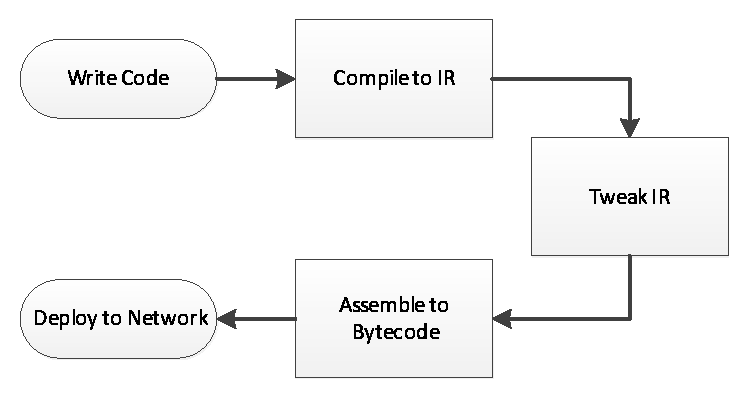
\includegraphics{Diagrams/predicate-dev-process.eps}
\caption{Workflow to create and deploy a user written predicate}
\label{fig:pred-workflow}
\end{figure}


\subsubsection{Domain Specific Language}

The following is the definition of how to parse our predicate language. We implemented it in Java using JavaCC, using several resources \footnote{JavaCC tutorial: \url{http://cs.lmu.edu/~ray/notes/javacc/}} to help in the development. Of the languages there are four main components. The first is the target of the predicate specified within square brackets, the target can be a node address (such as 1.0) or `all' to target all nodes in the network. The second is the function definitions. When users initialise our library on the motes, they need to provide a function that provides the current information on the node and a mapping of function ids to the functions used to access this data. The function definition statement in the predicate language allows a human understandable name to be assigned to a function id and it also tells the compiler what id function should be called and the type that that function returns. The third is the `using' statement that allows a set of neighbouring information to be assigned to a variable name. This is the only way to request node information not about the current node that is evaluating the predicate. The fourth and final part if the predicate itself, which includes expected logic operators that operate over sets, integers, floating point numbers and booleans. What is equivalent to what is described below.


\begin{table}[H]
\centering
\begin{tabular}{| l | l | l | l | l |}
\hline
Name & Logic Symbol & Our Symbol & Input Type(s) & Output Type\\
\hline

For All & $\forall$ & $\sm{@}$ & Sets of user defined data & Boolean\\
Exists & $\exists$ & $\sm{\#}$ & Sets of user defined data & Boolean\\

\hline

And & $\land$ & $\sm{\&}$ & Booleans & Boolean\\
Or & $\lor$ & $\sm{\textbar}$ & Booleans & Boolean\\
Xor & $\oplus$ & $\sm{\textasciicircum}$ & Booleans & Boolean\\
Implies & $\implies$ & $\sm{=\textgreater}$ & Booleans & Boolean\\
Equivalence & $\iff$ & $\sm{\textless=\textgreater}$ & Booleans & Boolean\\

\hline

Not & $\lnot$ & $\sm{!}$ & Boolean & Boolean\\

\hline

Equality & $=$ & $\sm{==}$ & Integers or Floats & Boolean\\
Inequality & $\not=$ & $\sm{!=}$ & Integers or Floats & Boolean\\
Less Than & $<$ & $\sm{\textless}$ & Integers or Floats & Boolean\\
Less Than or Equal To & $\leq$ & $\sm{\textless=}$ & Integers or Floats & Boolean\\
Greater Than & $>$ & $\sm{\textgreater}$ & Integers or Floats & Boolean\\
Greater Than or Equal To & $\geq$ & $\sm{\textgreater=}$ & Integers or Floats & Boolean\\

\hline

Addition & $+$ & $\sm{+}$ & Integers or Floats & Integer or Float\\
Subtraction & $-$ & $\sm{-}$ & Integers or Floats & Integer or Float\\
Multiplication & $\times$ & $\sm{*}$ & Integers or Floats & Integer or Float\\
Division & $\div$ & $\sm{/}$ & Integers or Floats & Integer or Float\\

\hline
\end{tabular}
\end{table}


\begin{eqnarray*}
	\pn{eval} & \pp & [ \pn{target} ] \ww \pn{function} \\
	\pn{target} & \pp & \sm{all} \\
	~ & \oo & \pn{number}\sm{.}\pn{number} \\
%
	\pn{function} & \pp & \sm{function} \ww \pn{number} \ww \sm{as} \ww \pn{string} \ww \sm{returning} \ww \pn{type} \ww \sm{in} \ww \pn{function} \\
	~ & \oo & \pn{using} \\
%
	\pn{using} & \pp & \sm{using} \ww \sm{Neighbours}\sm{(}\pn{number}\sm{)} \ww \sm{as} \ww \pn{variable} \ww \sm{in} \ww \pn{using} \\
	~ & \oo & \pn{predicate} \\
%
	\pn{predicate} & \pp &  \sm{(}\pn{predicate}\sm{)} \\
	~ & \oo & \pn{quantifier}\sm{(}\pn{variable} \ww \sm{:} \ww \pn{variable} \ww \sm{\mytilde} \pn{predicate} \sm{)}\\
	~ & \oo &  \pn{predicate} \ww \pn{logical-binary} \ww \pn{predicate} \\
	~ & \oo &  \pn{logical-unary} \ww \pn{predicate} \\
	~ & \oo &  \pn{var-expr} \ww \pn{math-logical-binary} \ww \pn{var-expr} \\
%
	\pn{var-expr} & \pp & \sm{(}\pn{var-expr}\sm{)} \\
	~ & \oo & \pn{number} \\
	~ & \oo & \pn{string}\sm{(}\pn{this-variable}\sm{)} \\
	~ & \oo & \pn{var-expr} \ww \pn{math-binary} \ww \pn{var-expr} \\
	~ & \oo & \sm{abs}\sm{(}\pn{var-expr}\sm{)} \\
	~ & \oo & \pn{set-fn}\sm{(}\pn{variable}\sm{)} \\
	~ & \oo & \pn{transform-set-fn}\sm{(}\pn{transform-fn}\sm{,} \ww \pn{variable}\sm{)} \\
%
	\pn{this-variable} & \pp & \pn{variable} \oo \sm{this} \\
	\pn{variable} & \pp & \pn{string} \\
%
	\pn{transform-fn} & \pp & \pn{string} \\
	\pn{transform-set-fn} & \pp & \sm{sum} \oo  \sm{mean} \oo \sm{max} \oo \sm{min} \\
	\pn{set-fn} & \pp & \sm{len} \\
%
	\pn{type} & \pp & \sm{float} \oo \sm{int} \\
%
	\pn{logical-binary} & \pp & \sm{\&}  \oo \sm{\textbar} \oo \sm{\textasciicircum} \oo \sm{=\textgreater} \oo \sm{\textless=\textgreater} \\
	\pn{logical-unary} & \pp & \sm{!} \\
	\pn{math-logical-binary} & \pp & \sm{==} \oo \sm{!=} \oo \sm{\textless} \oo \sm{\textless=} \oo \sm{\textgreater} \oo \sm{\textgreater=} \\
	\pn{math-binary} & \pp & \sm{+} \oo \sm{-} \oo \sm{*} \oo \sm{/} \\
%
%	\pn{string} & \pp & \pn{alpha}\pn{string-rest} \\
%	\pn{string-rest} & \pp & \nn \oo \pn{alpha}\pn{string-rest} \oo \pn{digit}\pn{string-rest} \\
%
%	\pn{alpha} & \pp & \sm{A}\dots\sm{Z} \oo \sm{a}\dots\sm{z} \\
%	\pn{number} & \pp & \pn{sign} \pn{number-first} \oo \pn{number-first} \\
%	\pn{number-first} & \pp & \pn{digit} \oo \sm{1}\dots\sm{9}\pn{number-rest} \\
%	\pn{number-rest} & \pp & \pn{digit} \oo \pn{digit}\pn{number-rest} \\
%	\pn{digit} & \pp & \sm{0}\dots\sm{9} \\
%	\pn{sign} & \pp & \sm{+} \oo \sm{-} \oo \nn \\
	\pn{quantifier} & \pp & \sm{@} \oo \sm{\#} \\
\end{eqnarray*}

When we were implementing the parsing for the predicate language one of the major issues encountered was that parsing infix operators (that is the operator is between two operands) was much harder to accomplish than prefix or postfix operators, \cite{ParsingRecursiveDescent} was used as a guide to implement infix parsing.

Another important issue to mention is the distinction between syntax and semanatics. The language definition specifies the syntax, but it fails to capture some of the semantic subtleties of valid programs. One example is that even if a variable name or a function name are syntactically valid strings, compilation should fail if they have not been defined by a statement prior to their usage. However, JavaCC provides a very capable framework for validating semantics during construction of the program's IR.

\subsubsection{Example Predicates}
\label{sec:example-predicates}

\begin{figure}[H]
\begin{minipage}{.5\linewidth}
\begin{lstlisting}[language=Hoppy]
[all]
function 1 as slot returning int in
    using Neighbours(2) as twohopn in
        @(x : twohopn ~
            slot(x) != slot(this)
        )
\end{lstlisting}
\end{minipage}%
\begin{minipage}{.5\linewidth}
\begin{align*}
&				\forall n \in \text{Nodes} \cdot \\
& \hspace{2em}		\forall n' \in \text{Neighbours}(n, 2) \cdot \\
& \hspace{4em}				\text{slot}(n) \neq \text{slot}(n')
\end{align*}
\end{minipage}

\caption{Check that no two neighbours have the same slot (2-hop information)}
\label{fig:two-hop-slot-pred-lang}
\end{figure}

\begin{figure}[H]
\begin{minipage}{.5\linewidth}
\begin{lstlisting}[language=Hoppy]
[all]
function 0 as addr returning int in
function 1 as slot returning int in
    using Neighbours(1) as onehopn in
        @(a : onehopn ~
            @(b : onehopn ~ addr(a) != addr(b)
                => slot(a) != slot(b))
            & slot(a) != slot(this)
        )
\end{lstlisting}
\end{minipage}%
\begin{minipage}{.5\linewidth}
\begin{align*}
&				\forall n \in \text{Nodes} \cdot \\
& \hspace{2em}		\forall n' \in \text{Neighbours}(n, 1) \cup \{n\} \cdot \\
& \hspace{4em}			\forall n'' \in \text{Neighbours}(n, 1) \cup \{n\} \cdot \\
& \hspace{6em}				\text{addr}(n') \not= \text{addr}(n'') \\
& \hspace{8em}					\implies \text{slot}(n') \neq \text{slot}(n'')
\end{align*}
\end{minipage}
\caption{Check that no two neighbours have the same slot (1-hop information)}
\label{fig:one-hop-slot-pred-lang}
\end{figure}


The predicates specified in \autoref{fig:two-hop-slot-pred-lang} and \autoref{fig:one-hop-slot-pred-lang} aim to check that slot allocation is correct and will not lead to collisions. As these are applications predicates they check that there are no clashes with the slots assigned. If we were also checking network related state, these predicates would also need to be monitoring the MAC layer to make sure that no collisions did in fact occur. Predicates similar to these appear in the problem statement of \cite{DBLP:journals/corr/abs-0808-0920}, which leads us to believe that an implementation of a TDMA algorithm may desire some checking of these predicates to test correctness of such an algorithm.

\begin{figure}[H]
\begin{minipage}{.5\linewidth}
\begin{lstlisting}[language=Hoppy]
[1.0]
function 3 as humidity returning float in
    humidity(this) <= 40.0
\end{lstlisting}
\end{minipage}%
\begin{minipage}{.5\linewidth}
\begin{align*}
&				\forall n \in Nodes \cdot \\
& \hspace{2em}		\text{addr}(n) = 1.0 \implies \\
& \hspace{4em}			\text{humidity}(n) \leq 40
\end{align*}
\end{minipage}
\caption{Check that the relative humidity of node 1.0 is less than or equal to 40\%}
\label{fig:app1-pred-lang}
\end{figure}

\begin{figure}[H]
\begin{minipage}{.5\linewidth}
\begin{lstlisting}[language=Hoppy]
[all]
function 2 as temperature returning float in
    using Neighbours(2) as twohopn in
        abs(temperature(this) - mean(temperature, twohopn)) <= 10
\end{lstlisting}
\end{minipage}

\begin{minipage}{.5\linewidth}
\begin{align*}
&				\forall n \in \text{Nodes} \cdot \\
& \hspace{2em}		\left|\text{temperature}(n) - \frac{\sum\limits_{n' \in \text{Neighbours}(n, 2)} \text{temperature}(n')}{|\text{Neighbours}(n, 2)|} \right| \leq 10
\end{align*}
\end{minipage}
\caption{Check that the average neighbour temperature is with 10 degrees of ours}
\label{fig:app2-pred-lang}
\end{figure}

The two predicates in \autoref{fig:app1-pred-lang} and \autoref{fig:app2-pred-lang} capture what system users may be trying to detect. \autoref{fig:app1-pred-lang} shows a predicate that fails when the humidity sensed by a predicate falls low and \autoref{fig:app2-pred-lang} detects when there is a large different in the temperature of one node and the average of its neighbours. Both of these predicates could be used when monitoring the environment in a forest to see how likely and where forest fires may be starting. 


\begin{figure}[H]
\begin{minipage}{.5\linewidth}
\begin{lstlisting}[language=Hoppy]
[all]
function 0 as addr returning int in
    using Neighbours(1) as onehopn in
    using Neighbours(2) as twohopn in
        @(a : onehopn ~
            #(b : twohopn ~ addr(a) == addr(b))
        )
\end{lstlisting}
\end{minipage}%
\begin{minipage}{.5\linewidth}
\begin{align*}
&				\forall n \in \text{Nodes} \cdot \\
& \hspace{2em}		\{\text{addr}(n') | n' \in \text{Neighbours}(n, 1)\} \subseteq \\
& \hspace{4em}			\{\text{addr}(n') | n' \in \text{Neighbours}(n, 2)\}
\end{align*}
\end{minipage}
\caption{Check 1-hop neighbourhood is in 2-hop neighbourhood}
\end{figure}

This predicate is perhaps not as interesting as other predicates but it has a valid use in testing certain aspects of the information dissemination aspect of our predicate checking algorithm. It is important that we can test our mechanisms to evaluate predicates, because if we cannot rely on the correct evaluation of predicates, then we cannot rely on the results. Predicates like checking the 1-hop neighbourhood is in the 2-hop neighbourhood allows us to check that we are gathering data in the right way.


\begin{figure}[H]
\begin{lstlisting}[language=Hoppy]
[all]
function 5 as sink-distance returning int in
    using Neighbours(1) as onehopn in
        sink-distance(this) == min(sink-distance, onehopn) + 1
\end{lstlisting}
\caption{We are one hop further from the base station than the closest of our neighbours. May be used to check parent in aggregation tree is actually closer to the sink.}
\label{fig:tree-agg-parent-hops-pred-lang}
\end{figure}

\begin{figure}[H]
\begin{minipage}{.5\linewidth}
\begin{lstlisting}[language=Hoppy]
[all]
function 0 as addr returning int in
function 4 as ch returning int in
function 6 as H returning int in
    using Neighbours(H(this)) as neighbours in
        #(node : neighbours ~
            ch(this) == addr(node)
        )
\end{lstlisting}
\end{minipage}%
\begin{minipage}{.5\linewidth}
\begin{align*}
&				\forall n \in \text{Nodes} \cdot \\
& \hspace{2em}		\exists n' \in \text{Neighbours}(n, \text{H}(n)) \cdot \\
& \hspace{4em}			\text{ch}(n) = \text{addr}(n')
\end{align*}
\end{minipage}
\caption{Check cluster head is in H-hop neighbourhood}
\label{fig:ch-in-H-hops-pred-lang}
\end{figure}

The predicate shown in \autoref{fig:tree-agg-parent-hops-pred-lang} and \autoref{fig:ch-in-H-hops-pred-lang} are examples of ways that we can use application predicates to check that the network communication aspect of wireless sensor network are working correctly. The first checks that a parent assigned in tree aggregation is closer to the sink than the evaluating node. \autoref{fig:ch-in-H-hops-pred-lang} is intended to check that there exists a cluster head within $H$ hops of the evaluating node. The aim would be to use this when hierarchical clustering is being used to perform routing. If either of these fail then the system administrators can simply rerun the configuration step to set up the communication paths or start looking for bugs in the code that performs this setup.

Unfortunately the predicate that checks the cluster head location would not work due to the fact that the parameter to \verb|Neighbours| needs to be known at compile time. This is an implementation issue and could be corrected in the future.


\subsection{Virtual Machine}

The virtual machine that was developed is very simple and takes inspiration from the wren \cite{wren} language's virtual machine. At heart our virtual machine uses a stack to evaluate a program, values can be pushed onto the stack and are then popped of the stack later for use in evaluation and the results of that evaluation are pushed back onto the stack. The last value on the stack is the results of the evaluation. In the virtual machine there are three types: 16-bit integers (I), 32-bit floats (F) and user-defined size user data (U). A boolean is represented as an integer with 0 standing for false and 1 standing for true, the virtual machine relies on the compiler to have generated correct code that will be correctly evaluated, it has limited error checking and reporting to keep the firmware size down.The virtual machine also has a limited and fix stack space that is configured to be 256 bytes. If this overflows then the predicate evaluation will be terminated with an error. Due to the limited space, predicates that require  more stack space than there is to evaluate themselves will fail. In testing these issues can be detected and the stack size can be increased as desired.

\subsubsection{Opcodes}

The program is stored as a block of memory that is a list of opcode followed by their arguments.

%\begin{verbatim}
\begin{lstlisting}[language=Dragon]
For binary operations the order the operands are used is specified as x op x.
When x is 0 the value on the top of the stack is used. When x is 1 the
value after the one on the top of the stack is used.

HALT
    Halts execution.
    The stack should always have at least one integer on it when halting.

IPUSH (int) / FPUSH (float)
    Pushes an int or a float on to the stack.

IPOP / FPOP
    Pops the stack by sizeof(int) or sizeof(float) bytes.

IFETCH (variable id - ubyte) / FFETCH (variable id - ubyte)
    Fetches the value of the given variable and pushes the
    first sizeof(int) or sizeof(float) bytes of it on to the stack.

ISTORE (variable id - ubyte) / FSTORE (variable id - ubyte)
    Stores the first sizeof(int) or sizeof(float) bytes in the variable
    of the given name.

AFETCH (variable id - ubyte)
    Fetches the value of the array named in the parameter
    at the integer index at the top of the stack.

ALEN (variable id - ubyte)
    Pushes an integer onto the stack containing the length
    of the named array.
	
ASUM  (variable id - ubyte) (function id - ubyte)
AMEAN
AMAX
AMIN
    Over the user defined array stored in the variable whose
    name is the first parameter, transform it using the function
    whose name is the second parameter. On this transformed data
    calculate the array operation and push the result as a float
    onto the top of the stack.

CALL (function id - ubyte)
    Calls the named function on the data on top of the stack.
    Pop's the data that was given to the function off the top of
    the stack (sizeof(U)) and pushes the result onto the top of the stack.

ICASTF
    Pops an integer off the stack, casts it to a float
    then stores it back on the stack.

FCASTI
    Pops a float off the stack, casts it to a integer
    then stores it back on the stack.

JMP (ubyte)
    Jumps to a position in the code relative to the start
    of the program.

JZ (ubyte)
    Pops and reads the top of the stack as an integer, if it is 0
    the program jumps to the location, otherwise evaluation
    continues.

JNZ (ubyte)
    Pops and reads the top of the stack as an integer, if it is not 0
    the program jumps to the location, otherwise evaluation
    continues

IADD / FADD       1 op 0
ISUB / FSUB        1 op 0
IMUL / FMUL        1 op 0
IDIV1 / FDIV1       0 op 1
IDIV2 / FDIV2       1 op 0
    Performs a mathematical operations on the first two sizeof(int) or sizeof(float)
    values on the stack. Pops both values off the stack, stores
    the result in the same type back on the stack.

IINC
IDEC
    Pops the top of the stack by sizeof(int) bytes, increments or decrements
    the value as an integer. Pushes the result back on the stack

IEQ / FEQ	        1 op 0
INEQ / FNEQ        1 op 0
ILT / FLT        1 op 0
ILEQ / FLEQ        1 op 0
IGT / FGT	        1 op 0
IGEQ / FGEQ        1 op 0
    Performs a mathematical operations on the first two sizeof(int) or sizeof(float)
    values on the stack. Pops both values off the stack, stores
    the result in an integer on the stack.

AND         1 op 0
OR          1 op 0
XOR	        1 op 0
EQUIVALENT  1 op 0
IMPLIES     1 op 0
    Performs a logical operation on the first two values on the
    stack. These are not bitwise operations and the expected
    formats of the values are integers. 0 is false, 1 is true.
    Pops both values off the stack,
    stores the result in an integer back on the stack.

NOT
    Pops an integer off the stack, performs logical not on it.
    Pushes the result back on the stack.
	
IVAR (variable id - ubyte) / FVAR (variable id - ubyte)
    Creates a variable of type int or float with the id set to the given
    unsigned byte.

IABS / FABS
    Pops the stack by sizeof(int) or sizeof(float) bytes performs the abs function
    on the integer of float value and pushes sizeof(int) or sizeof(float) back onto
    the stack.

VIINC (x - variable id)
    Equivalent to the following opcodes, this is opcode is included as
    a program size optimisation.
    IFETCH x
    IINC
    ISTORE x

VIDEC (x - variable id)
    Equivalent to the following opcodes, this is opcode is included as
    a program size optimisation.
    IFETCH x
    IDEC
    ISTORE x

VIFAFC (x - variable id) (y - variable id) (z - function id)
    Equivalent to the following opcodes, this is opcode is included as
    a program size optimisation.
    IFETCH x
    AFETCH y
    CALL z

THISC (f - function id)
    This opcode gets the sizeof(U) bytes about the nodes current state,
    calls the function referred to by f on it and pushes that result onto the stack.
    This is equivalent to:
    IPUSH 0
    AFETCH 0
    CALL f
\end{lstlisting}
%\end{verbatim}


\subsubsection{Bytecode}

One of the most important aims of the predicate language's bytecode was to be as small as possible. The reason for this was to support sending as much program information in the limited length of a network packet. To achieve this aim it meant that we needed to make the virtual machine handle more abstract representations of its components. For example, initially the bytecode for calling a function contained a byte for the opcode of \verb|CALL| and then a string of characters which contained the name of the function to call. At minimum this would cost 2 bytes - one for the character of the function's name and one for the NUL character. To improve this the string was replaced with a single byte, which means that the number of functions callable by the virtual machine ends up being limited to 256. The same was true for the variable ids as well and as the variable id is contained with an unsigned byte, they to are limited to 256.

Size optimizations were also done for operations we believed would be common. This is why there exists the \verb|ASUM|, \verb|AMEAN|, \verb|AMIN| and \verb|AMAX| operations. If these were to be coded they would at least require a loop and a certain amount of setup code that loops require. By making them single operations we can eliminate the need to produce loops in the IR and can just produce these single instructions. Also as these instructions are much simpler they make adjusting the IR easier and harder to introduce bugs. The unfortunate downside is that this means that there is more implementation in the virtual machine which leads to increased firmware sizes.

The firmware size restrictions did eventually lead to a number of features being removed. For example, during development we had support for calculating the power and modulus of variables. However, due to the size of the C libraries that were pulled in to use the \verb|pow| function, it needed to be disabled. The modulus function was also disabled as it has a rare use case and the firmware space was needed for actual implementation of the application.


When developing the virtual machine what also became important was the fact that the bytecode was a string of unsigned bytes, where sequences of them could end up representing a 16 bit integer or a 32 bit float. This is important because it could mean that we would try to perform unaligned reads which the CPU of our motes could potentially get wrong\footnote{\url{http://permalink.gmane.org/gmane.os.contiki.devel/1462}}, this is due to the restrictions the CPU has on the alignment of words: ``Bytes are located at even or odd addresses. Words are only located at even addresses \ldots. When using word instructions, only even addresses may be used. The low byte of a word is always an even address'' \cite[Section~1.4.5 (p.~28)]{msp430usersguide}.

\begin{figure}[ht!]
\centering
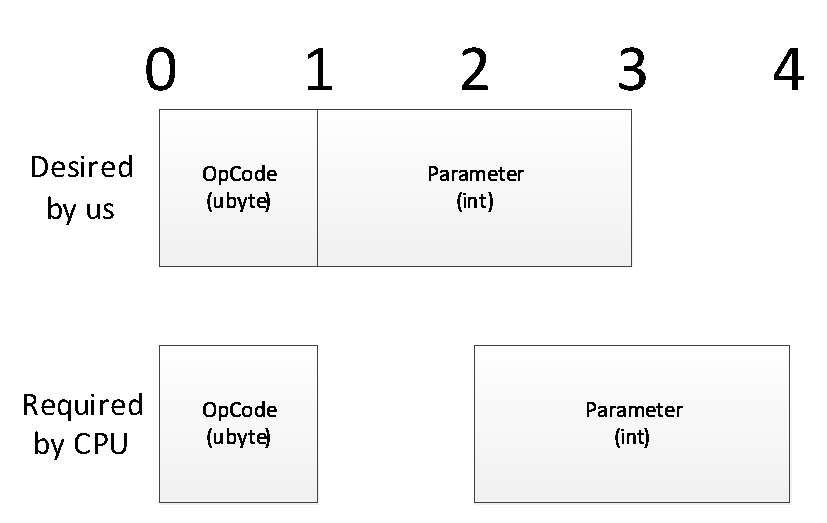
\includegraphics[scale=0.75]{Diagrams/byte-alignment.eps}
\caption{Alignment Issues}
\label{fig:alignment-issues}
\end{figure}

\begin{figure}[ht!]
\begin{verbatim}
[java] **** Illegal read - misaligned word from $2c01 at $80de
[java] Stack Trace: number of calls: 4 PC: $80de
[java] evaluate (errno.c) called from PC: $7166
[java] process_thread_mainProcess (local in pred-eval.c) called from PC: $bf12
[java] call_process (local in process.c) called from PC: $c0b2
[java] process_run (errno.c) called from PC: $4250
\end{verbatim}
\caption{Example of the error messages produced by MSPSim in Cooja that led to the discovery of this bug}
\end{figure}

As can be seen in \autoref{fig:alignment-issues} if we were to align the words as the CPU wanted the size of the bytecode would massively increase as every single byte bytecode would need to be padded by a byte to (i) make sure all bytecode entries were the same length and to ensure the word parameters are correctly aligned. To solve this issue instead of accessing the memory directly in the bytecode what can be done instead is to copy the memory out byte-by-byte into a correctly aligned block of memory and use that instead. As we copy out byte-by-byte and not by word we can access the memory correctly.

\subsection{Examples of Compiled Programs}

\begin{figure}[H]
\begin{minipage}{0.65\linewidth}
\hrule
\begin{lstlisting}[language=Hoppy]
[all]
function 1 as slot returning int in
    using Neighbours(2) as twohopn in
        @(x : twohopn ~
            slot(x) != slot(this)
        )
\end{lstlisting}
\begin{lstlisting}[language=Dragon]
//TARGETING all
//FUNC 1 AS slot
//STORING 2 IN twohopn
IVAR 1
IPUSH 1
IPUSH 0
ISTORE 1
start1: ALEN 255
INEQ
JZ end1
//slot(a[*1])
VIFAFC 1 255 1
//slot(this)
THISC 1
INEQ
AND
VIINC 1
JMP start1
end1: HALT
//VD 2 = 255
\end{lstlisting}
\hrule
\begin{lstlisting}[language=Hoppy]
[all]
function 0 as addr returning int in
function 1 as slot returning int in
    using Neighbours(1) as onehopn in
        @(a : onehopn ~
            @(b : onehopn ~ addr(a) != addr(b)
                => slot(a) != slot(b))
            & slot(a) != slot(this)
        )
\end{lstlisting}
\end{minipage}\hspace{1em}
\begin{minipage}{0.25\linewidth}
\begin{lstlisting}[language=Dragon]
//TARGETING all
//FUNC 0 AS addr
//FUNC 1 AS slot
//STORING 1 IN onehopn
IVAR 1
IPUSH 1
IPUSH 0
ISTORE 1
start1: ALEN 255
INEQ
JZ end1
IVAR 2
IPUSH 1
IPUSH 0
ISTORE 2
start2: ALEN 255
INEQ
JZ end2
//addr(a[*1])
VIFAFC 1 255 0
//addr(b[*2])
VIFAFC 2 255 0
INEQ
//slot(a[*1])
VIFAFC 1 255 1
//slot(b[*2])
VIFAFC 2 255 1
INEQ
IMPLIES
AND
VIINC 2
JMP start2
//slot(a[*1])
end2: VIFAFC 1 255 1
//slot(this)
THISC 1
INEQ
AND
AND
VIINC 1
JMP start1
end1: HALT
//VD 1 = 255
\end{lstlisting}
\end{minipage}
\caption{Compiled check for slot collisions. Using 2-hop information of \autoref{fig:two-hop-slot-pred-lang} on the left and using 1-hop information of \autoref{fig:one-hop-slot-pred-lang} on the right.}
\label{fig:two-hop-slot-pred-lang-compiled}
\end{figure}

Here we can see the vast difference that is caused by using a single loop versus a nested loop. The single loop program that uses two hop information as an assembled binary size of 28 bytes, whereas the assembled size of the one hop information program has a size of 68 bytes. This program size may eventually become important when reaching the maximum allowed size of a single packet, as it is unlikely that a program like this will be able to go much over 100 bytes (without support for splitting the program up).

Also included in the programs are comments placed there by the compiler to indicate what the code is doing, the aim is that the developers will be able to manually tweak the code to try to reduce the size of it. Perhaps one of the startling differences is the benefit of some of the special array opcodes as can be seen in \autoref{fig:app2-pred-lang-compiled} which is only 13 bytes long. Without the \verb|AMEAN| opcode there would need to be a loop in IR to calculate the mean, by shifting this responsibility to the interpreter the code size can reduced by eliminating an interpreted loop.

\begin{figure}[H]
\begin{minipage}{0.7\linewidth}
\begin{lstlisting}[language=Hoppy]
[all]
function 2 as temp returning float in
    using Neighbours(2) as twohopn in
        abs(temp(this) - mean(temp, twohopn)) <= 10
\end{lstlisting}
\end{minipage}
\begin{minipage}{0.2\linewidth}
\begin{lstlisting}[language=Dragon]
//TARGETING all
//FUNC 2 AS temp
//STORING 2 IN twohopn
//temp(this)
THISC 2
AMEAN 255 2
FSUB
FABS
IPUSH 10
ICASTF
FLEQ
HALT
//VD 2 = 255
\end{lstlisting}
\end{minipage}
\caption{Compiled mean temperature check of \autoref{fig:app2-pred-lang}}
\label{fig:app2-pred-lang-compiled}
\end{figure}

One final optimisation that is worth mentioning is that, while we have support for it, we will often not generate code that involves pushing floats onto the stack. This is because if it is possible it we can save a byte of the program size by instead pushing an integer and then casting it to a float. When pushing a float we need 1 byte for the opcode and 4 bytes for the float being pushed giving 5 bytes of program. In the optimised case we need 1 byte for the \verb|IPUSH| opcode, 2 bytes for the integer and 1 byte for the \verb|ICASTF| opcode giving 4 bytes of program instead of 5.


\subsection{Testing}

As the virtual machine and its parsers can be fairly complex and difficult pieces of code to understand it was very important that we had test cases that validated that the functionality was correct. To do this three sets of tests are performed. Of them two are unit tests, one that tests that assembled bytecode can be correctly executed and the other that tests that the parser/compiler can correctly parse and generate code. After this is an integration test, that checks if the output of the parser/compiler converted into bytecode by the assembler can be correctly executed. To test the correct execution set data is given to the virtual machine, which can then be used in the predicates.

Different things are tested for each of the integration tests. When testing the assembler and virtual machine, short programs of opcodes are provided to test simple activities such as pushing onto the stack, calling functions or arithmetic. This is simply to test the functionality of the virtual machine. As we can be sure that the functionality is correct, when testing the compiler more complex predicates that we have designed the system to use are tested. We expect that for some of these tests scripts the code would be the same for real world uses.



\subsection{Data Transmission}

So far we have covered what we wish to evaluate and how that shall be evaluated, however, we have not talked about how data shall reach its destination to be evaluated. The how of evaluating data is split into two parts: `where' the predicate should be evaluated and `when' the data should be disseminated.

Regarding where a predicate should be evaluated there seem to be two choices. Either there is collection of all the networks state at a single location designated as a sink (such as the base station), this is what traditional Global Predicate Evaluation algorithms would do. Or, the predicate could be evaluated in the network at some target node. We intend to investigate both of these.

Considering when the data should be disseminated there are again several options available. The first and most obvious is to simply periodically send out the information. However, periodic data transmission could potentially inefficient, so we will also investigate event-based dissemination. Finally, nodes could also request information when it is desired. We investigate all three of these.

\begin{table}[H]
\centering
\begin{tabular}{| l | m{5cm} | m{5cm} |}
\hline
~ & Local & Global \\
\hline
Periodic & Periodically asks neighbours for information & Periodically aggregates information to sink \\
\hline
Event & Periodically checks for changes, on change floods information locally &  Periodically checks for changes, on change aggregates data to sink \\
\hline
\end{tabular}
\caption{Description of predicate evaluation behaviours}
\end{table}


\subsubsection{Local Event}

When gathering data in-network using an event-based update mechanism and evaluating the predicate locally in-network there two things of importance. The first and simplest is knowing that data has changed. Because there are no ways to plug into the OS and receive notifications that a section of memory has changed it means that the local data needs to be checked periodically for a change. To do this the function that the library user has provided to return the node data will be called and then compared against some history. This history is simply the last piece of data that was sent into the network. A comparison function needed to be supplied by the user because doing a simple comparison of the memory may lead to change events being fired even though values have not changed. There are several examples where this is important. The first is that floating point calculations can produce different representations of the same results, bitwise the values may differ but logically the values are the same. Another case is that many sensors have a tolerance associated with them, by checking the values with a function this tolerance can be taken into account and events will not be fired if the data has not changed significantly. Finally, using a tolerance function allows the library user to specify the difference that is meaningful to them, even if it is different to the sensor tolerance.

As we check periodically to detect a change and then fire events, it means that there is still the possibility that we will miss some changes. For example a sensor value may spike in between measurements and this may never be detected due to how the checking period aligns with the spikes.

When an event is fired that indicates that the node's data has changed it means that the data will need to be sent to some of the nodes in the network. Our implementation simply floods the information the maximum number of hops a predicate is asking for data. For example if there are 3 predicates in the network using 1-hop, 2-hop and 4-hop data, every node will flood their data 4-hops when it changes. This solution works because every node keeps a record of all the predicates in the network even if they are not evaluated by every node.

There is the potential for optimisations here by using knowledge of the node's neighbours to detect if a node actually needs the current nodes data and then only flooding the data if that is the case. For example if there is one predicate in the system that is targeted to a single node that needs 3-hop information, but the node whose data has just changed is 4 hops away, that node would not need to send its information. However, this would mean that every node would need an accurate picture of the network state. This may be energy intensive to calculate, so we leave this optimisation to be investigated in later work.

\begin{figure}[H]
\centering
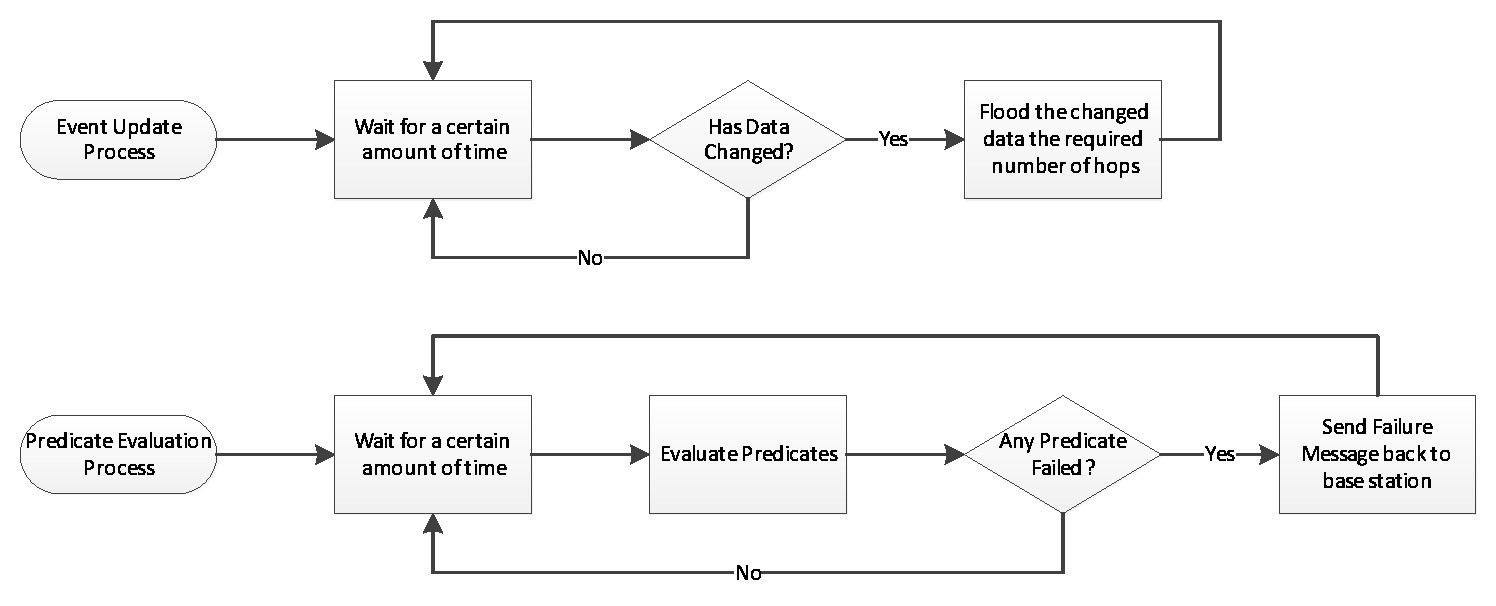
\includegraphics[width=\linewidth]{Diagrams/pele.eps}
\caption{Predicate Evaluation Local Event (PELE)}
\end{figure}

\subsubsection{Local Periodic}

The major difference between evaluating data periodically when evaluating a predicate in-network is that instead of data being sent to nodes when it changes, data is only sent to nodes when it is requested. The idea is that when a node is evaluating its predicates it finds the maximum distance it needs information for and floods a message that many hops asking for data and each of those nodes reply back along the path that the request message came from. After a node evaluates all its predicates for that period it then forgets all that information. The reason this is done is because in the event based dissemination there is no ability to detect changes in topology and remove invalid data. For example say a cluster head that has successfully delivered information in the past crashes. As that information has been delivered and is only updated when it changes all the nodes simply assume that the data remains the same and will continue evaluating the predicate as if the cluster head had not crashed. Neighbours of the failed cluster head could detect and send this information, but as that involves network information it is not an application predicate and is out of the scope of this work. So the solution was to simply consider the information available at the node evaluating a predicate at that instant.

Instead of requesting information every node could simply periodically broadcast it. However, that has the disadvantage of causing nodes to broadcast information when they don't need to (a problem from event-based dissemination) and also could lead to problems when nodes clocks are perfectly aligned. For example nodes could consistently receive old information from nodes if they keep sending data that was meant for a previous round such that is it only received during the current round of predicate evaluation. By asking for data these issues are mitigated.

\begin{figure}[H]
\centering
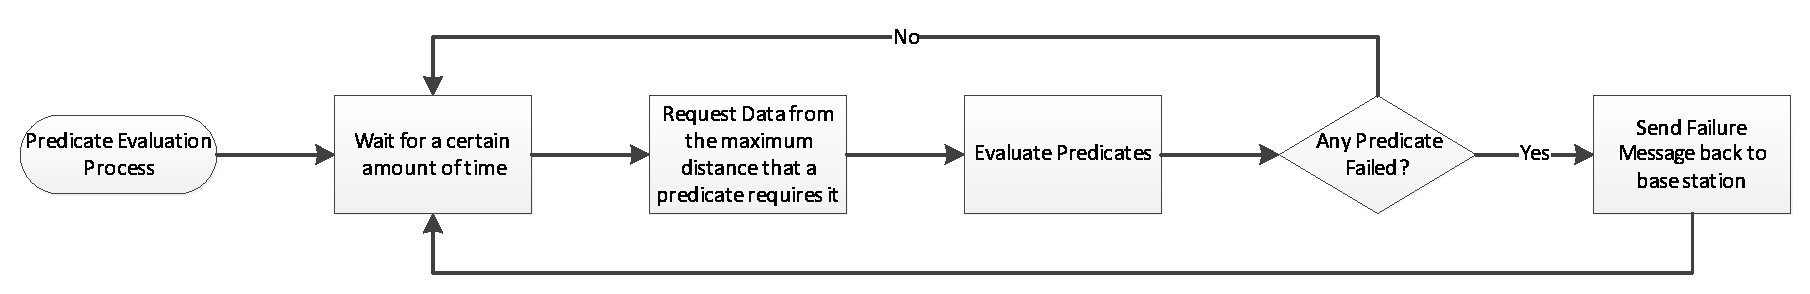
\includegraphics[width=\linewidth]{Diagrams/pelp.eps}
\caption{Predicate Evaluation Local Periodic (PELP)}
\end{figure}

When using the N-Hop Request library to implement this predicate evaluator there is an important issue that needs to be considered: when we have sent the data request message how long should we wait for? We cannot simply wait until all the results are returned to the evaluating node because (i) we do not necessarily know what node's data we will be waiting for and (ii) we may not receive that data anyway. We could wait for $2 \times D \times T_{send} + \epsilon$ time units, where $D$ is the maximum number of hops we are asking for information from, $T_{send}$ is the amount of time it takes for a message to try to be sent and $\epsilon$ is a small extra amount of time to wait. However, knowing what $T_{send}$ is can be difficult, and is based on many complicated factors. For example, if the MAC protocol in use uses CSMA/CD or CSMA/CA then it is possible, when trying to send a message, to enter into an arbitrary number of back-off period while waiting for the channel to be free \cite{?}. If there is an upper bound on the number of retries then we can calculate a maximum $T_{send}$, otherwise we cannot. Therefore, for our implementation we chose to use a fixed large value in which it was reasonable to expect all the responses that would return, would return within that period. We expect that in the future, this wait period will need to be some function of $D$ the number of hops of information being asked for to support requesting information from deeper in the network.


\subsubsection{Global}

When considering evaluating predicates at a sink, the data can simply be aggregated to it along a tree. For both event-based and periodic data generation the way the data is generated can remain the same, the requesting of data is simply removed (for periodic) and instead of flooding the information to neighbours it is aggregated instead.

However, this change causes a few knock-on effects. For the aggregation of neighbours and data in PEGP the behaviour is as expected, data is generated at the leaves and aggregated onwards towards the tree's root node where it is used. When aggregating data that is generated in PEGE, it is not the leaves that periodically generate data. Instead every node could potentially cause a message to being being forwarded through the tree. The big change is that every time a packet is forwarded the current node's data is aggregated to with it. This means that nodes closer to the root node of the tree have more opportunities to aggregate their data. Overall we do not believe this will affect the evaluation behaviour, as in the worst case more recent information may be available when it might not otherwise have been so.

The biggest issue with the global style of predicate evaluation is the latency that is introduced between gathering the data from the nodes in the network and the evaluation of the predicate. One problem is that the data in the network may have changed since it was gathered, a larger problem is that data will be compared at potentially very different times due to the aggregation delays. This was not as much of an issue with local in-network evaluation because the data was quickly flooded back to the target node. However, with tree aggregation every hop towards the sink needs a long wait to gather as much data as possible to reduce number of messages sent. This could potentially lead to a number of predicates being incorrectly evaluated by using data from different times.

\begin{figure}[H]
\centering
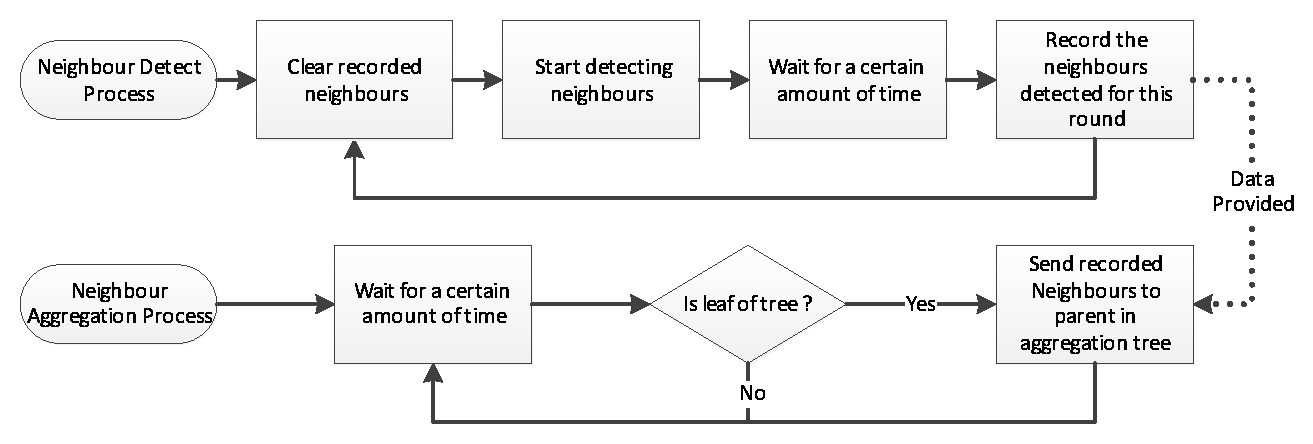
\includegraphics[width=\linewidth]{Diagrams/pegx-neighbour-agg.eps}
\caption{Neighbour Aggregation used for global predicate evaluation}
\end{figure}

Both the event-based and period versions of global predicate evaluation require the two processes of neighbour detection and aggregation running. Initially we planned to use this data to visualise the state the network is in. However, it turns out that it is a vital component of global predicate evaluation. Without this information we would be unable to work out how many hops  the data is from the node that is currently being evaluated.

As every predicate is evaluated is evaluated at the root of the aggregation tree, it becomes necessary for that root node to be able to pretend that they are the node where the predicate would usually have been evaluated. This is so the relevant neighbours can be used, and also so the virtual machine will use the correct data for the $this$ variable.

\begin{figure}[H]
\centering
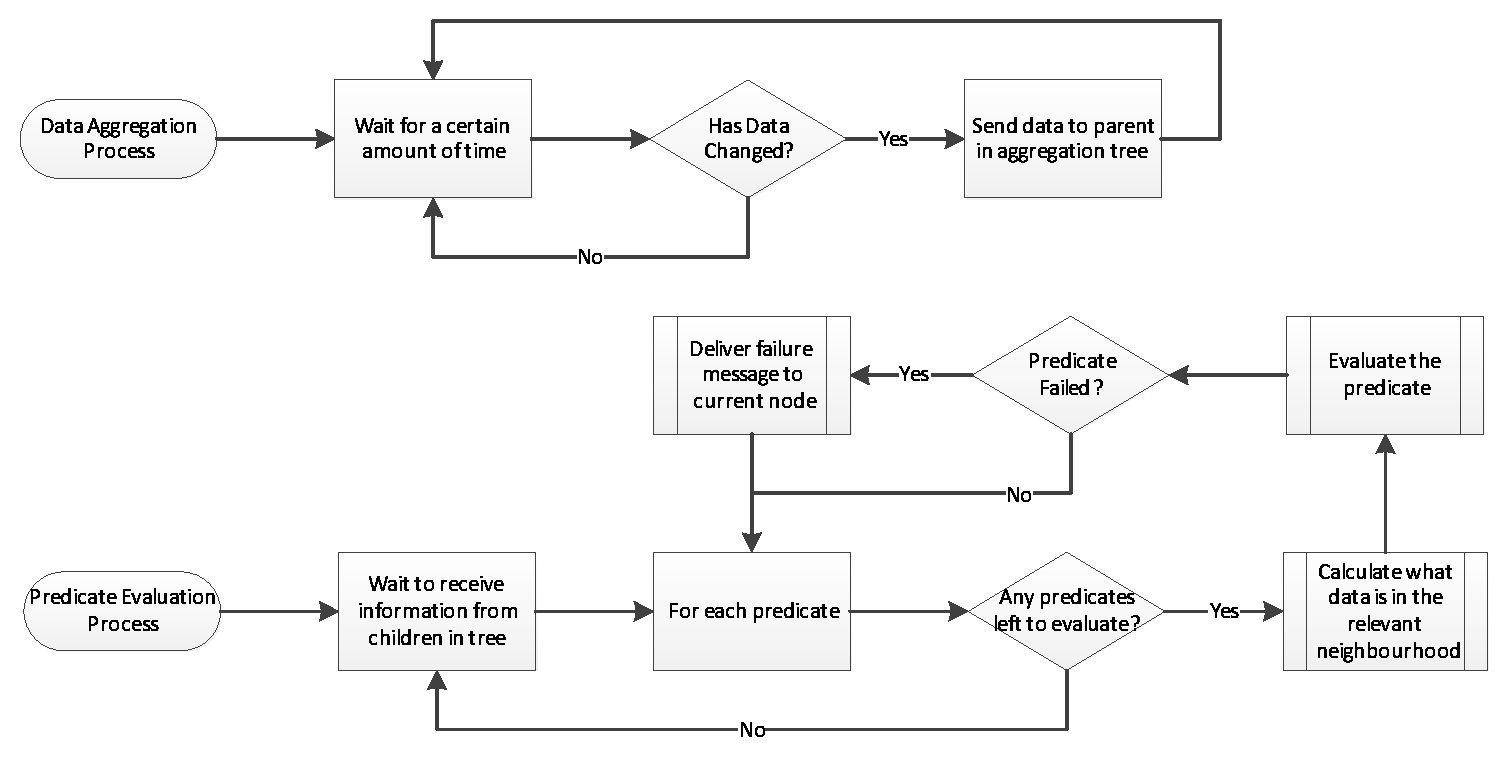
\includegraphics[width=\linewidth]{Diagrams/pege.eps}
\caption{Predicate Evaluation Global Event (PEGE)}
\end{figure}

Between the two versions of global predicate evaluation there are only minor differences in how the algorithm is implemented. The first is that when sending data PEGE checks to see if the data has changed before sending it, PEGP instead checks if the node is a leaf in the tree and relies on the aggregation of intermediate nodes to gather all the network's data. The second is a consequence of the first difference, PEGE will keep and update the information it receives. PEGP instead only used the last round of information that has been received. So after every predicate has been evaluated at the end of a predicate evaluation round the node information is cleared. This feature was added to enable support for (untested) handling failures in the network such as crashes or for handling the case when the nodes are mobile.

\begin{figure}[H]
\centering
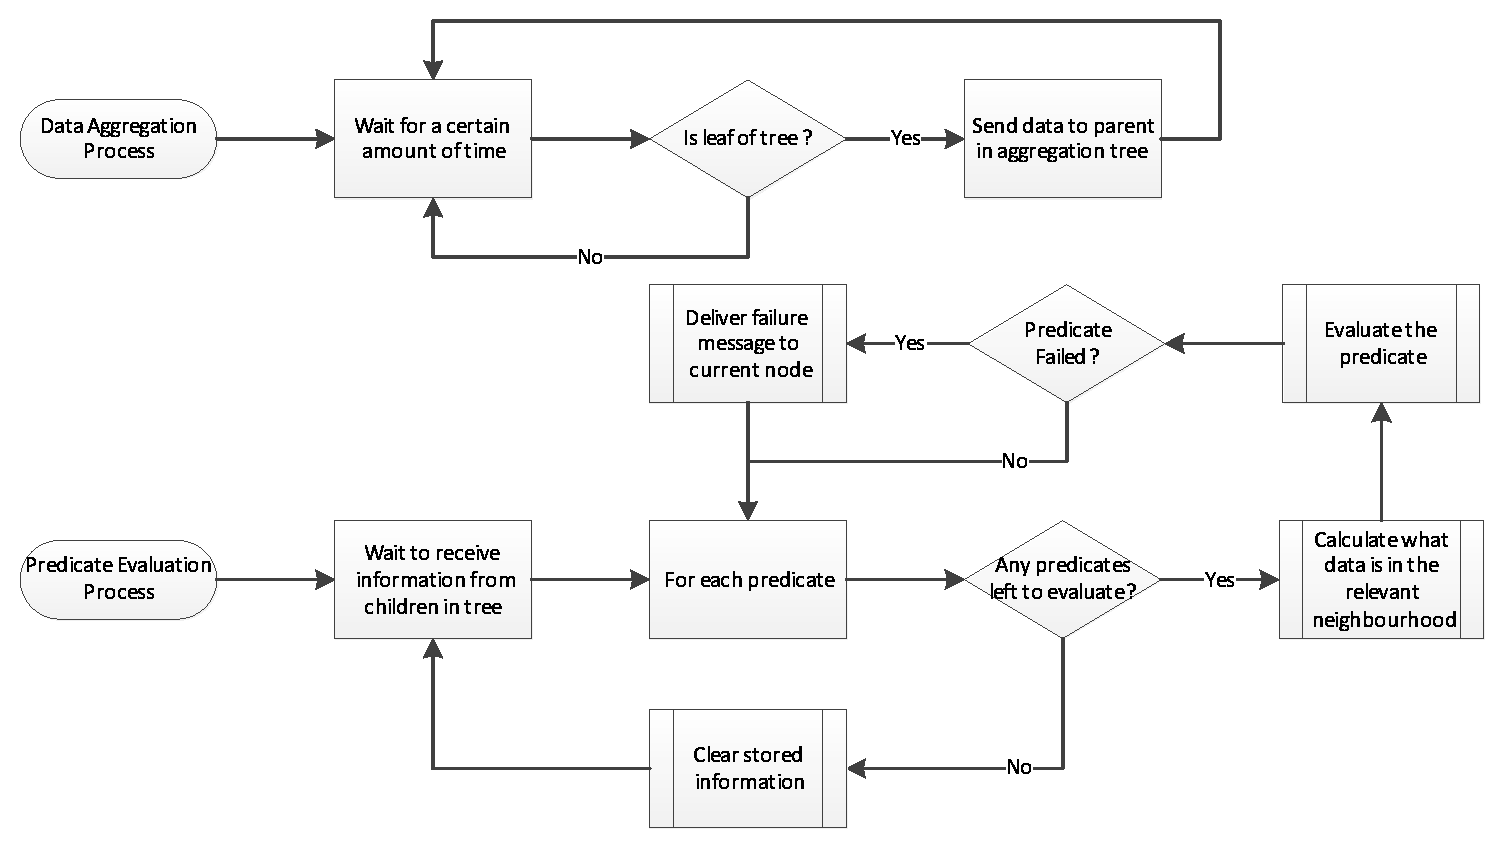
\includegraphics[width=\linewidth]{Diagrams/pegp.eps}
\caption{Predicate Evaluation Global Periodic (PEGP)}
\end{figure}


\subsubsection{Reply}

Once a node has reached the point of having a result after evaluating a predicate it needs to do something meaningful with that information so that users looking for results at the base station also end up knowing this information. The first and most obvious solution would be to inform the base station of every result, be it success or failure. Unfortunately while this is the most comprehensive response it is would also require the most energy as every node would need to send a repose message for every predicate they were evaluating.

\begin{equation}
C = |P_{all}| \times |V| + |P_{single}|
\end{equation}

The alternatives are to either send a message when a predicate has failed or when a predicate succeeds. This allows only a fraction of $C$ messages to be sent. However, there are a number of differences that make deciding to send success or failure an important decision. First of all is how the result is represented. The comprehensive solution has the advantage that the result of a predicate can be put into an \emph{unknown} state. Once a result message is received the result of that predicate can be moved into a \emph{failed} or \emph{succeeded} state. For success or failure messages you would need to assume the opposite of the messages that you are waiting for (i.e. assume predicates failed before receiving the succeeded message and vice versa) and change the state once the message is received. If messages are lost then this will lead to false notifications of success when waiting for failure messages and false failures when waiting for success messages.

The other issue to consider is what should be reported. If success messages are the chosen form of the response, then what useful information could they contain? One would expect the state that the predicate was evaluated with, but this information is not nearly as useful as the state that caused a predicate to fail. Another factor is that to create a useful description of why an error message failed is complex and would require more resources than simply evaluating the message. This means that practically it would be best for a failure message to report the state that caused the predicate to fail back to the base station and then expect further analysis on it there.

As we expect a predicate failure to be an infrequent event, our libraries have been designed to report only predicate failures. This should save energy in the form of messages. However, we expect the system to be vulnerable to not showing the full extent failures (falsely appearing successful), when messages are lost.


\subsection{A Consideration}

One of the main examples provided was the problem of assigning slots in a TDMA MAC protocol, where one would wish to ensure that no node within two hops of any given node has the same slot. Interestingly there are multiple ways to structure the predicate to perform this evaluation.


The first predicate we might consider is the one where for every node, we get the 2-hop neighbourhood and check that none of those nodes have the same slot as the initial node. This means that we would need to send:
\begin{enumerate}
	\item A message from the base station to the node asking it to evaluate the predicate
	\item A message from the node to each of its 2-hop neighbours
	\item Each 2-hop neighbour needs to send a message back to the node
	\item The node would need to wait for its neighbours to send the messages, then evaluate the predicate. This would imply that the node would need to know who is in its two hop neighbourhood
	\item The node would need to report to the base station the result of the predicate
\end{enumerate}

So we would need at best $|V| + \Delta_{sink}(n) + M(P)$ messages to evaluate this predicate for the single node $n \in V$. We need $|V|$ message to flood the predicate to every node, $\Delta_{sink}(n)$ is needed to send a failure reply back to the sink and the last component $M(P_{2})$ is the message cost of evaluating the predicate on that node. For example $M(P_{2}) = 2|Neighbours(n, 1)|$ for PELP as a message has to be flooded out two hops to ask for the information and then those nodes need to respond.

\begin{align}
\label{eq:2-hop-slot-pred}
& 				\forall n \in \text{Nodes} \cdot \\
& \hspace{2em}		\forall n' \in \text{Neighbours}(n, 2) \cdot \\
& \hspace{4em}			\text{slot}(n) \neq \text{slot}(n')
\end{align}

The second predicate we could consider is the one where every node checks their 1-hop neighbourhood for slot collisions. Here we model the 2-hop nature of the predicate differently, because instead of checking on the node that we want to check for slot collisions, we check on the node between two nodes that might have slot collisions.

\begin{enumerate}
	\item A message from the base station to the nodes adjacent to that we asking to check slot collisions
	\item A message from the node to each of its 1-hop neighbours
	\item Each 1-hop neighbour needs to send a message back to the node
	\item The node would need to wait for its neighbours to send the messages, then evaluate the predicate. This would imply that the node would need to know who is in its two hop neighbourhood
	\item The node would need to report to the base station the result of the predicate
\end{enumerate}

Initially one may consider that this 1-hop predicate can simply be evaluated on a node $n' \in V$ where $\{n, n'\} \in E$. However, this means that this predicate is no longer equivalent to that 2-hop predicate. For example if $n$ has another neighbour $n''$ whose 1-hop neighbourhood is not contained within $n'$'s 1-hop neighbourhood ($Neighbours(n'', 1) \setminus Neighbours(n', 1) \not= \emptyset$) then $n''$ would also need to be checked.

So the number of message that would be required to evaluate this 1-hop predicate on the required node is  $|V| + \sum_{n' \in Neighbours(n, 1)}{\Delta_{sink}(n')} + M(P_{1})$. Where $|V|$ is required for the same reasons as the 2-hop predicate and every neighbour $n'$ of $n$ needs to send a failure message. $M(P_{1}) = \sum_{n' \in Neighbours(n, 1)}{2|Neighbours(n', 1)|}$ for PELP because every neighbour $n'$ of $n$ needs to ask $n'$'s 1-hop neighbourhood for information.


\begin{align}
\label{eq:1-hop-slot-pred}
&				\forall n \in \text{Nodes} \cdot \\
& \hspace{2em}		\forall n' \in \text{Neighbours}(n, 1) \cup \{n\} \cdot \\
& \hspace{4em}			\forall n'' \in \text{Neighbours}(n, 1) \cup \{n\} \cdot \\
& \hspace{6em}				\text{addr}(n') \not= \text{addr}(n'') \implies \text{slot}(n') \neq \text{slot}(n'')
\end{align}

So this introduction of the 1-hop predicate has led to a spreading out of the evaluation, but with roughly the same amount of energy usage. The energy usage is roughly the same as the number of nodes from which data is requested is the same in $M(P_{1})$ as $M(P_{2})$. However, the 1-hop implementation has a good advantage, which is that by asking nodes neighbouring the 1-hop neighbours of $n$ to also evaluate the predicate they can take advantage that some of the predicate is already being evaluated. As shown in \autoref{fig:1-hop-new-eval} a new node can be set to evaluate a predicate and that node will take advantage of the already evaluated neighbouring information that is not necessary to repeat. Whereas the 2-hop predicate would need to repeat a lot of data request and evaluation if it were to be evaluated on multiple nodes. So Adding more and more nodes that evaluate the 1-hop predicate will scale much better than the 2-hop predicate simply because the of way that the evaluation is distributed and the way that distribution can prevent duplicate requesting of information. So checking an entire network for slot collisions should be much more energy efficient when using the 1-hop predicate.


\begin{figure}[H]
\centering
\subfigure[Checking green node has no slot collisions]{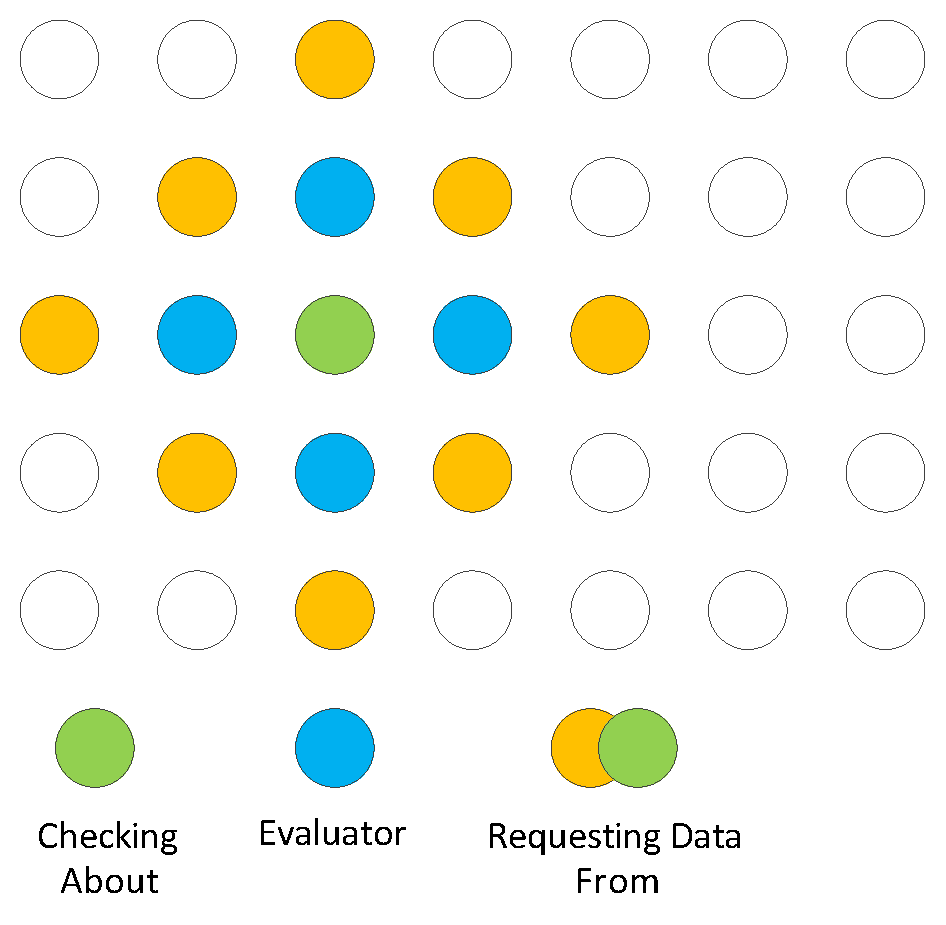
\includegraphics[width=0.4\linewidth]{Diagrams/1-hop-checking-a.eps}}\hspace{3em}
\subfigure[Adding new evaluators to check new node has no slot collisions]{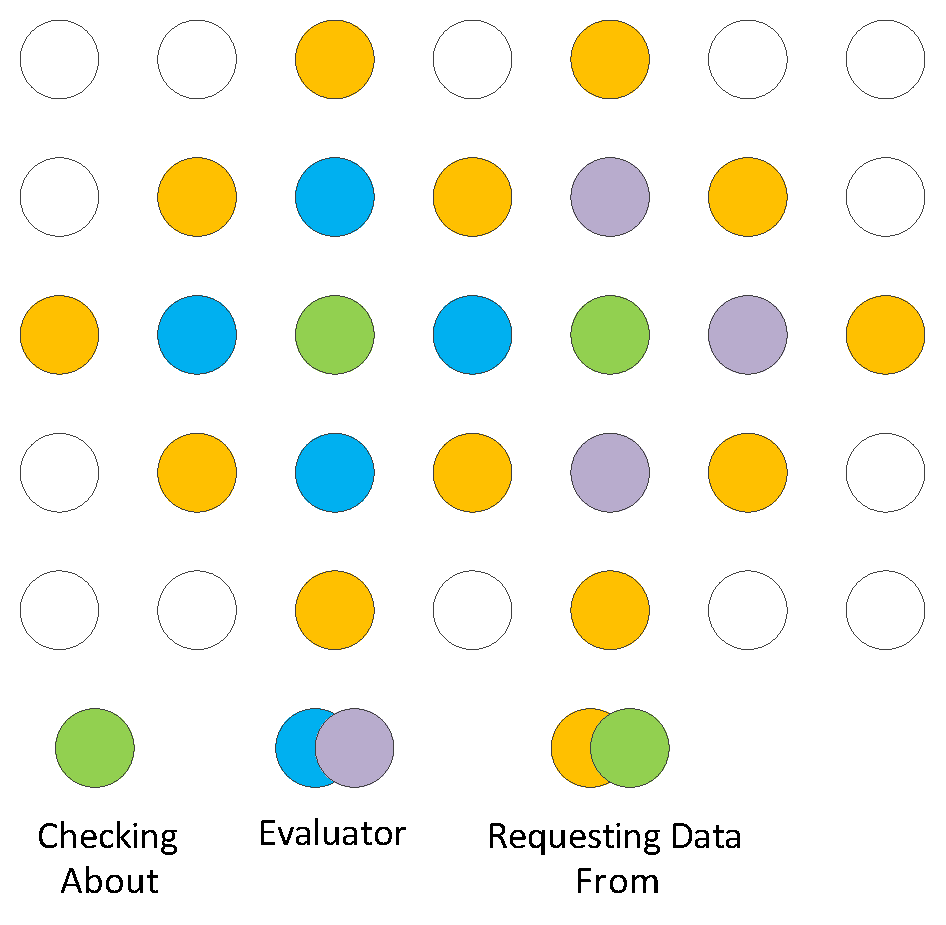
\includegraphics[width=0.4\linewidth]{Diagrams/1-hop-checking-b.eps}}
\caption{Utilising the 1-hop predicate structure to add new evaluators}
\label{fig:1-hop-new-eval}
\end{figure}


However, there is one final factor to take into account that even though using 2-hop information will require more energy it is the simpler predicate - it only has a single loop with a simpler check. This predicate requires 28 bytes instead of the 68 bytes that the predicate that required 1-hop information uses. When predicates get larger and more complicated it may be important that they can be expressed in a simpler way that may perhaps use more energy, but also are smaller and need less stack space to be evaluated. If the cost of performing a firmware update across the network is very high and would be needed to support larger predicates, then the energy cost of the simpler predicate may end up being worth it.

\subsection{A Distance Issue}

% Problem of Distance(n, n')

The only network primitive we have implemented is a function that gets information on nodes within a certain number of hops of the asking node. There are a number of other network primitives that might be useful for both network and application predicates. One of these is the ability to get the distance between two nodes.

An example of a predicate that uses $Neighbours(n, h)$ is shown below. This predicate is for Hierarchical Clustering where $H$ is a parameter that defines the distance between cluster heads. The predicate checks that for every node there is a neighbour in the $H$-hop neighbourhood that is a cluster head.

\begin{align*}
& \hspace{2em}	\forall n \in Nodes \cdot \\
& \hspace{4em}		\exists n' \in Neighbours(n, H) \cdot \\
& \hspace{6em}			IsClusterHead(n)
\end{align*}

An alternative way that we might specify this predicate is to check that the distance between a node and the cluster head (that it knows the address of) is within $H$ hops.

\begin{align*}
& \hspace{2em}	\forall n \in Nodes \cdot \\
& \hspace{4em}		IsClusterHead(n) \lor Distance(n, ClusterHead(n)) \leq H
\end{align*}

However, there is an issue with this predicate. How would we implement the $Distance(n, n')$ primitive? With $Neighbours(n, h)$ we know how far we need to ask for information ($h$ hops), with $Distance(n, n')$ the maximum distance that we will need to wait for information to return from is the diameter of the network. Unfortunately we cannot assume that the diameter is known. If instead we take a time-out approach there is no way that we can guarantee to wait for the correct amount of time. For example if we wait enough time to check if a node is at maximum $D$ hops from the given node the node will need to wait for  time units. However, if the node we are trying to find the distance of is at $D + 1 $ hops then we will not believe the two nodes are connected. To reliably wait to check if two nodes are connected in a network where the diameter is not known we will need to wait for $\infty$ time units. Thus making $Distance(n, n')$ impossible to implement without knowing the diameter. Due to this issue we have not implemented such a network primitive function.


\subsection{Optimising on Predicate Structure}

% Conjuntive vs disjuntive predicates


When evaluating predicates in-network, it possible to consider optimisations due to the structure of the predicate to reduce the amount of information that is requested. For example take conjunctive predicates where the structure of the predicate $P$ is $P = P_1 \land P_2 \land \ldots \land P_n$. If one of the $P_i$ is false then the result of the predicate $P$ is false ($False \land P \Leftrightarrow False$). This means that the statements could potentially be evaluated in an order such that the $P_i$ that requires the fewest resources is evaluated first and the $P_j$ that requires the most resources is evaluated last.

The aim of this optimisation is to reduce energy usage by sending fewer messages. For the two types of data gathering in-network and at the sink, when gathering this data at the sink it would not be of any use as the data is sent to the sink in an event-based or periodic way. The sink doesn't ask for this information, so it is not possible for it to not ask for certain pieces of data. This is also true of event-based in-network predicate checking. So the only time this optimisation would be of use to us is when gathering data for in-network predicates that are checked periodically.

%Surprisingly, asking for and receiving all the required information actually requires fewer messages than incrementally asking for information. This is because of the communication that needs to be repeated when asking for more information. For example if you have a conjunctive predicate where the sub-predicates require 1 and 3 hops of information. If we ask for all information then we simply send messages out 3 hops and then receive replies from all the nodes in that neighbourhood. If we instead ask for one-hop information first and then three-hop, we first have to send a message to local neighbours and then will end up sending them another data request message when asking for three-hop information (as the 1-hop neighbourhood is contained within the 3-hop neighbourhood).

For some predicates it may make obvious sense to implement such an optimisation, such as if there is a conjunctive predicate that needs 1-hop information and 15-hop information. If the 1-hop predicate is often false, then it saves asking for information from all nodes that are within 15 hops of the evaluating node. However, as many of the predicates are not likely to require information from that distance (we expect one to two hops, with the possibility of three hops) it is an optimisation that would not serve to optimise what we are targeting our system to evaluate. Another issue is that many of the predicates we have thought up are not of this form, they mostly have quantifiers as the outer structure with other logical operators inside that quantifier. It may be the case where you have a predicate of the following structure $P = P_{local} \land \land P_{network}$ where $P_{local}$ needs no network information, here there is the possibility to optimise the network request out if $P_{local}$ is false. However as adding this feature would increase the firmware size we decided against adding more optimisations. This was because the software began to reach the limit of the firmware size when the virtual machine was integrated with the message communication. However, investigating these kinds of optimisations is a future possibility.

%
%\begin{figure}[H]
%\begin{equation}
%\sigma(x) = \sum_{i=1}^{x} i \times |N(i)|
%\end{equation}
%\caption{The number of messages required to respond x hops}
%\end{figure}
%
%The sigma function is defined as it is because for each of the nodes that are $x$ hops away they will require sending their data message $x$ hops to reach the requesting node.
%
%\begin{figure}[H]
%\begin{equation}
%\sum_{j \in H} |N_F(j)| + \sigma(j)
%\end{equation}
%\caption{Maximum number of messages for an incremental data request}
%\end{figure}
%
%\begin{figure}[H]
%\begin{equation}
%|N_F(\text{max}(H))| + \sigma(\text{max}(H))
%\end{equation}
%\caption{Number of messages for a complete data request}
%\end{figure}







\clearpage

% !TeX root = Report.tex
\section{Results}

\subsection{Methodology}

In our simulations we tested networks of various sizes (15, 30 and 48 nodes) aligned in a grid. The nodes were placed such that every node had four neighbours, one to the north, south, east and west, except for nodes in the edge which had three neighbours and the nodes in the corner that had two neighbours. The sink was always placed in the top left corner and was always assigned the address ``1.0''. The predicate checking algorithm was started as soon as the nodes had come online, the nodes then waited for 5 minutes to allow the predicate checking algorithm time to setup and then the TDMA algorithm was started. The simulation was run for 35 minutes overall and then it was terminated. After the predicate checking algorithm had setup the predicate was checked every 4 minutes.

To gather metrics on the energy usage of the motes, a Contiki library called rimestats was used. This library is built into the MAC layer and records deep statistics, we simply used the sent and received message counts. In order to calculate how much energy the TDMA algorithm was using we implemented our own sent and received counters that were incremented when a message was sent or received. As the TDMA protocol was implemented with simple broadcasts there should be a one-to-one correspondence between the number of successful broadcasts and the number of transmissions done at the MAC layer, the same is also true for when receiving a message. To calculate the energy cost of the predicate evaluation algorithm, the difference between the total and the TDMA energy usage was taken.

To check that a predicate was successfully evaluated the TDMA algorithm printed any changes in the assigned slot as well as the time the slot was changed. When a predicate was evaluated on a node the time it was evaluated as well as the result was printed. Analysis scripts then evaluated the predicate using the most recent slot value from before or up to when the predicate was evaluated to evaluate the predicate itself. This result was then compared with the actual result of the predicate. The results were compared whether or not the predicate response message reached the sink.

We ran these experiments using two different predicates, one that required 1-hop information and one that required 2-hop information. Both were checking to see if there were slot collisions and were the same two predicate that were mentioned as examples in \autoref{sec:example-predicates}. Below the code and logic for the two predicates is reproduced.

\begin{figure}[H]
\begin{minipage}{.5\linewidth}
\begin{lstlisting}
[all]
function 1 as slot returning int in
    using Neighbours(2) as twohopn in
        @(x : twohopn ~
            slot(x) != slot(this)
        )
\end{lstlisting}
\end{minipage}%
\begin{minipage}{.5\linewidth}
\begin{align*}
&				\forall n \in \text{Nodes} \cdot \\
& \hspace{2em}		\forall n' \in \text{Neighbours}(n, 2) \cdot \\
& \hspace{4em}				\text{slot}(n) \neq \text{slot}(n')
\end{align*}
\end{minipage}

\caption{Check that no two neighbours have the same slot (2-hop information)}
\label{fig:two-hop-slot-pred-lang-results}
\end{figure}

\begin{figure}[H]
\begin{minipage}{.5\linewidth}
\begin{lstlisting}
[all]
function 0 as addr returning int in
function 1 as slot returning int in
    using Neighbours(1) as onehopn in
        @(a : onehopn ~
            @(b : onehopn ~ addr(a) != addr(b)
                => slot(a) != slot(b))
             & slot(a) != slot(this)
        )
\end{lstlisting}
\end{minipage}%
\begin{minipage}{.5\linewidth}
\begin{align*}
&				\forall n \in \text{Nodes} \cdot \\
& \hspace{2em}		\forall n' \in \text{Neighbours}(n, 1) \cup \{n\} \cdot \\
& \hspace{4em}			\forall n'' \in \text{Neighbours}(n, 1) \cup \{n\} \cdot \\
& \hspace{6em}				\text{addr}(n') \not= \text{addr}(n'') \\
& \hspace{8em}					\implies \text{slot}(n') \neq \text{slot}(n'')
\end{align*}
\end{minipage}
\caption{Check that no two neighbours have the same slot (1-hop information)}
\label{fig:one-hop-slot-pred-lang-results}
\end{figure}

\subsection{Analysis}

\begin{figure}[H]
\centering
\subfigure[Rx]{%
	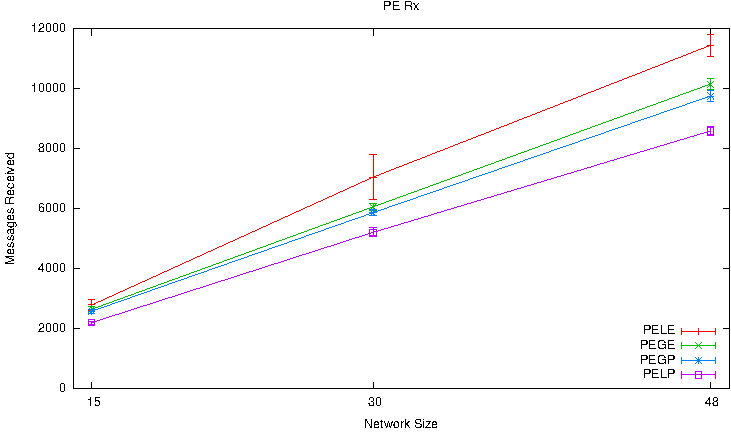
\includegraphics[width=0.44\linewidth]{../Results/Graphs/4.0/1HOP/messagesPE/rx/graph.pdf}
	\label{fig:predeval4.0-rx}
}
\subfigure[Tx]{%
	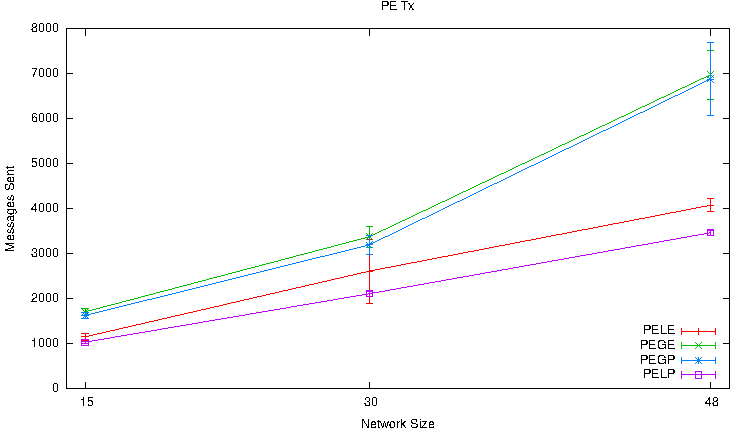
\includegraphics[width=0.44\linewidth]{../Results/Graphs/4.0/1HOP/messagesPE/tx/graph.pdf}
	\label{fig:predeval4.0-tx}
}

\subfigure[Percentage of  predicates correctly evaluated]{%
	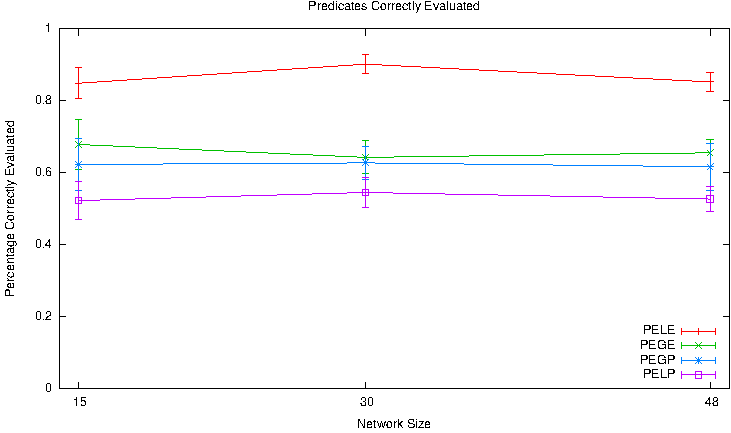
\includegraphics[width=0.44\linewidth]{../Results/Graphs/4.0/1HOP/pcCorrectlyEvaluated/graph.pdf}
	\label{fig:predeval4.0-correct}
}
\subfigure[Percentage of responses received]{%
	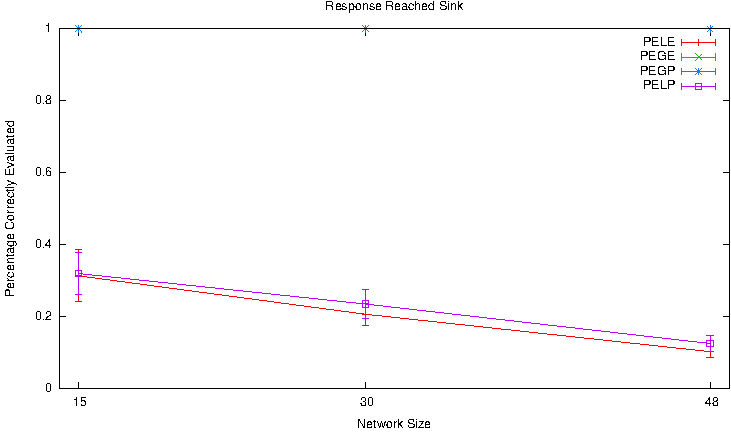
\includegraphics[width=0.44\linewidth]{../Results/Graphs/4.0/1HOP/pcResponsesReachedSink/graph.pdf}
	\label{fig:predeval4.0-recv}
}
\caption{Results when predicate period is every 4.0 seconds using a 1-hop predicate}
\label{fig:predeval4.0}
\end{figure}

The first point of note from the data presented in \autoref{fig:predeval4.0} is that in \subref{fig:predeval4.0-recv}, is that both of the global predicate evaluation algorithms (PEGE and PEGP) show a 100\% delivery rate. While this may initially appear very impressive, this simply arises from the facts that these predicates are evaluated at the sink, and that the graph shows the receipt of evaluated predicates sent from the evaluation location to the sink -- as no messages need to be sent, it is vacuously true that no messages will fail to arrive. The two local predicate checking algorithms, however, showed a more predictable trend of successfully delivering fewer responses as the network size increased, though the specific values of these rates are disappointingly low. The values suggest that only nodes in the immediate environs of the sink are being successful in sending the results of their predicate evaluations (perhaps a consequence of the mesh routing protocol used for sending this information). As the network grows in size, the proportion of nodes within this range of the sink decreases, resulting in the trend shown.

Graph \subref{fig:predeval4.0-correct}, showing the rate of correct predicate evaluation, reveals much more useful information: locally-evaluated event-triggered predicates show significantly higher accuracy than each of the other algorithms. Global event-based predicates was shown to have the second-highest accuracy, though this accuracy was only slightly higher than that of its periodic counterpart so it cannot be concluded that an event-based approach is universally better (within the scope of this metric). There may be a connection between PELE having the highest number of received messages (graph (a)) and its superior accuracy in evaluation; the premise being that more messages being received could give a node more data to use when evaluating a given predicate, in turn making it more likely to return a correct response. This notion of higher message delivery rates for PELE is somewhat corroborated by the number of transmissions shown in \subref{fig:predeval4.0-tx} -- PELE is responsible for the second lowest number messages sent. However, the cause of PELE alone having a significantly higher success rate in delivering messages is as yet unknown, so more definitive information on this front would require further scrutiny using testing methods that may well prove infeasible in a resource-constrained system.

As messages sent and received use the most energy in a WSN system \cite{?} we will use message transmit and receive statistics to evaluate the energy usage of the algorithms. In graphs \subref{fig:predeval4.0-rx} and  \subref{fig:predeval4.0-tx}), local periodic predicate evaluation is the most conservative, however it also shows the lowest accuracy for its evaluations so these results show little in the way of benefits to using this algorithm. By contrast, the most accurate algorithm, PELE, has a higher (yet still moderate) level of energy consumption. An important observation is that the energy demands of global predicate evaluation -- both of which showed middling accuracy -- increase faster than those of local evaluation as network size increases. This is because global evaluation requires data from the entire network, and the operating of the mesh routing protocol means that nodes lying further from the sink will have to have their messages forwarded by a greater number of intermediate nodes, giving exponential growth in the number of messages sent. The local evaluation algorithms show a more scalar trend as the size of a node's 1- or 2-hop neighbourhood may not increase due to the presence of more nodes in the network -- all that is guaranteed is that there will be more such neighbourhoods in which to evaluate predicates.

\begin{figure}[H]
\centering
\subfigure[Rx]{%
	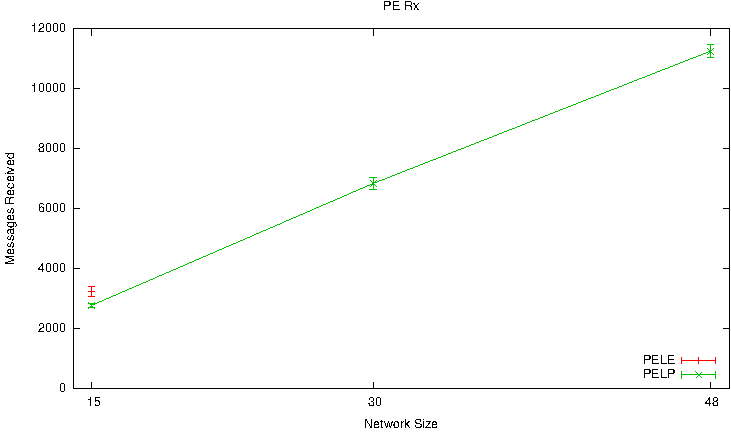
\includegraphics[width=0.44\linewidth]{../Results/Graphs/2.0/1HOP/messagesPE/rx/graph.pdf}
}
\subfigure[Tx]{%
	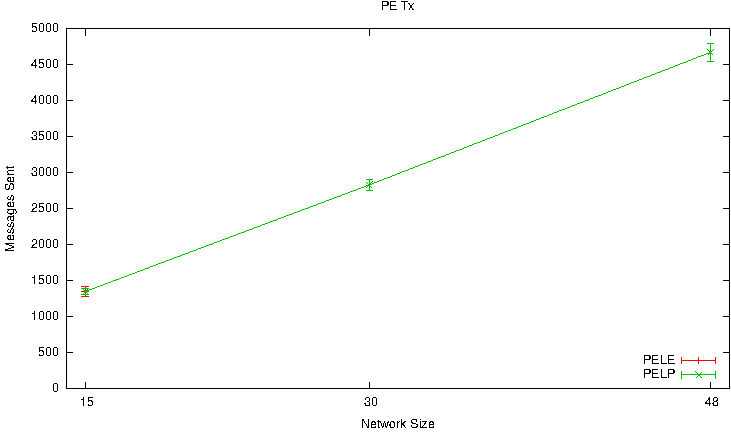
\includegraphics[width=0.44\linewidth]{../Results/Graphs/2.0/1HOP/messagesPE/tx/graph.pdf}
}

\subfigure[Percentage of predicates correctly evaluated]{%
	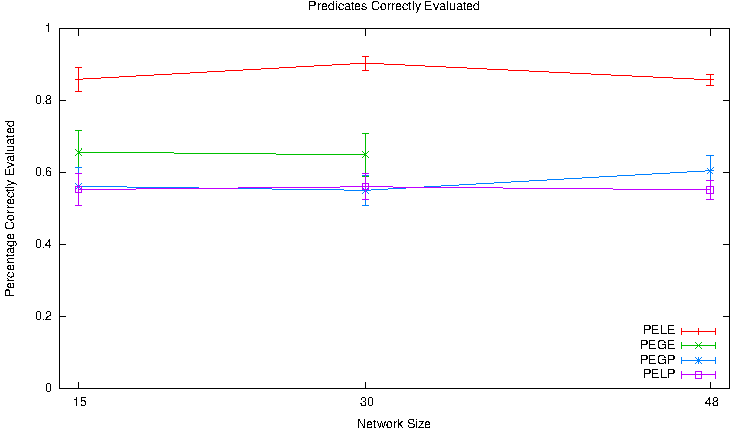
\includegraphics[width=0.44\linewidth]{../Results/Graphs/2.0/1HOP/pcCorrectlyEvaluated/graph.pdf}
}
\subfigure[Percentage of responses received]{%
	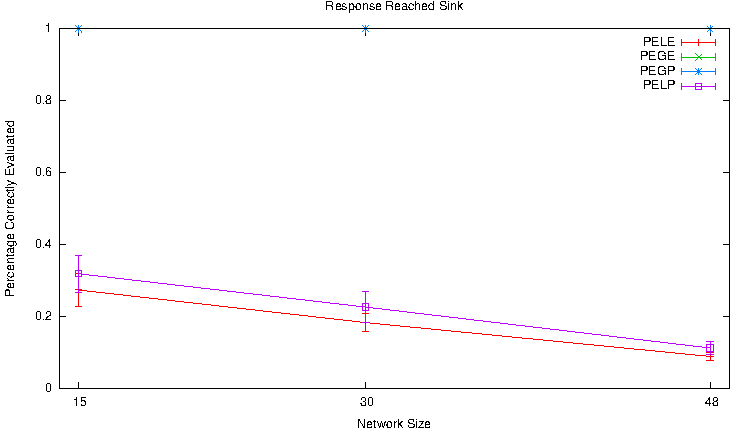
\includegraphics[width=0.44\linewidth]{../Results/Graphs/2.0/1HOP/pcResponsesReachedSink/graph.pdf}
}
\caption{Results when predicate period is every 2.0 seconds using a 1-hop predicate}
\end{figure}

\begin{figure}[H]
\centering
\subfigure[Rx]{%
	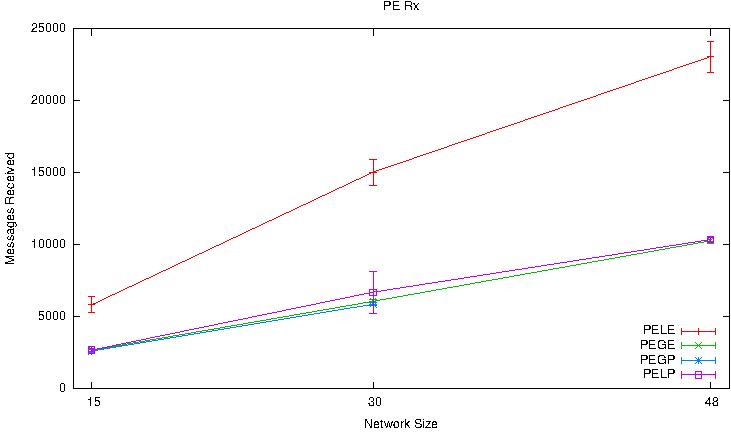
\includegraphics[width=0.44\linewidth]{../Results/Graphs/4.0/2HOP/messagesPE/rx/graph.pdf}
}
\subfigure[Tx]{%
	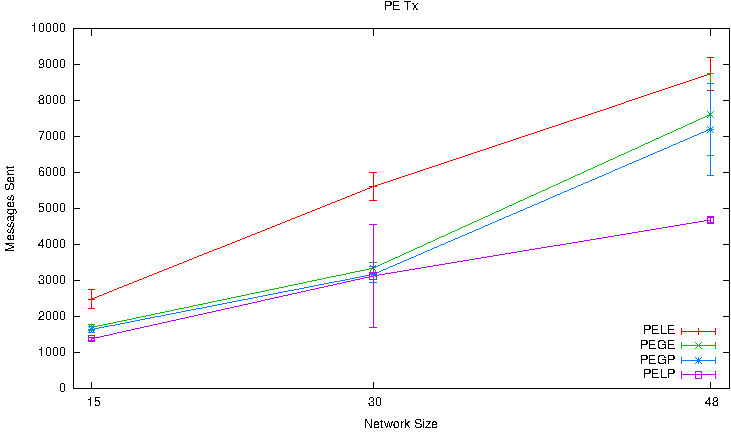
\includegraphics[width=0.44\linewidth]{../Results/Graphs/4.0/2HOP/messagesPE/tx/graph.pdf}
}

\subfigure[Percentage of predicates correctly evaluated]{%
	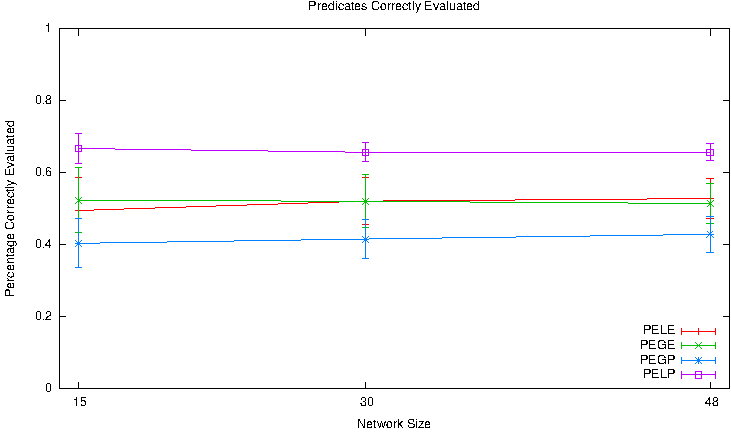
\includegraphics[width=0.44\linewidth]{../Results/Graphs/4.0/2HOP/pcCorrectlyEvaluated/graph.pdf}
}
\subfigure[Percentage of responses received]{%
	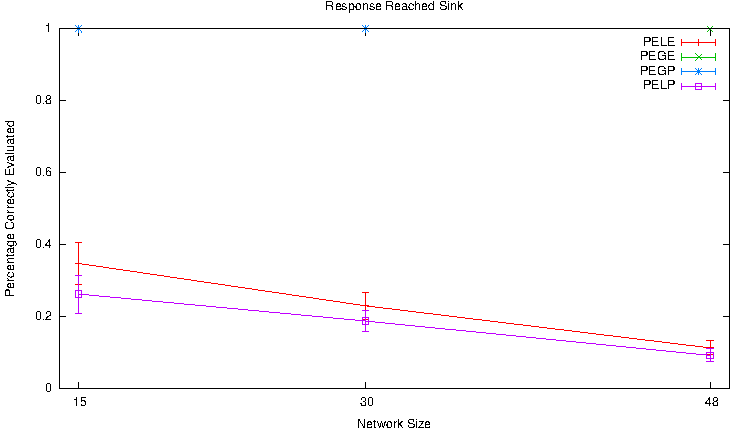
\includegraphics[width=0.44\linewidth]{../Results/Graphs/4.0/2HOP/pcResponsesReachedSink/graph.pdf}
}
\caption{Results when predicate period is every 4.0 seconds using a 2-hop predicate}
\end{figure}


\clearpage

% !TeX root = Report.tex
\section{Practical Experience}

As part of this project we learnt a number of things that we feel would be useful to impart on anyone else that undertakes development of wireless sensor networks with Contiki and physical hardware. Many of the issues we encountered were simply down to poor documentation or it being located in difficult to find places. We hope that the information included in this section is helpful.

\subsection{Contiki Logical Channels}

One of the first confusing aspects of Contiki is that when creating connections you need to provide a channel number. Initially we believed that this channel caused the messages being sent by that connection to be broadcasted on a different frequency to. However, after some research we found that the channels are in fact virtual \cite{Dunkels:2007:ACA:1322263.1322295,tel-aviv-contiki-exercises}. By virtual we mean that the same radio frequency is used to broadcast and receive all messages, but when when a packet is received it is funnelled to the correct receiver by way of the channel included in the packet. If one wishes to change the frequency of the radio, the function \verb|cc2420_set_channel| should be used. There are many other functions capable of changing settings in the cc2420 radio header \footnote{core/dev/cc2420.h \url{http://contiki.sourceforge.net/docs/2.6/a00158_source.html}}. Another example API is \verb|cc2420_set_txpower| which allows the transmission power of the radio to be set.

\subsection{Power Levels}

As mentioned in the previous section there exists an API that can be used to set the transmission power of the radio (\verb|cc2420_set_txpower|). We experimented using the hardware in the Computer Science building at the University of Warwick at different power levels. This was done because ideally we wished to experiment deploying the applications to the hardware and then testing them in a real world environment. The reason that we needed to investigate power levels was so that we could control the neighbourhood of motes to be a small space, otherwise we would have been very spread out through the building making it difficult to update motes as necessary. Unfortunately at the low transmission power that would allow nodes to communicate when within 15cm of one another but not when further away, we found that very few messages were received by nodes. We believe that this was caused by the environment that we were testing in (DCS building), as we expect the traffic on the 2.4GHz frequency to be very busy due to the number of phones and wireless devices in the department. Therefore, we recommend to do as many other who investigate sensor networks do, and test in remote areas away from interference from commonly used devices \cite{?}.


\subsection{Sensor Data Conversion}

The sensors attached to our hardware did not provide results in a binary format such as an integer or a float. This meant that we had to convert from their custom binary representation to the binary representation desired. Equations were provided by the manufacturer to perform these conversions \cite{sensiriondatasheet}, however, constants in those equations are heavily dependant on the specifications of the sensor (such as the voltage levels and the number of bits of data the sensor reports). So we recommend making sure that the correct constants are used by comparing the results of the sensor to a known accurate measuring device - such as a thermometer.

\subsection{Uploading to the motes}

When uploading the code to the motes there is a good amount of documentation on how to do so. However, there are a certain number of other steps that need to be taken. Below is the line of code that needs to be entered into the terminal. This will make the code and it is important that a \verb|make clean| has been run on the command line before hand. The \verb|.upload| at the end of the project name informs the name script to upload to the motes and the \verb|MOTES| variable is used to locate the USB port the mote is connected to.

\begin{listing}
\begin{minted}[fontsize=\small]{bash}
sudo make example-unicast.upload DEFINES=DUMMY,NODE_ID=1 MOTES=/dev/ttyUSB0
\end{minted}
\caption{Command to upload firmware to a mote connected to a USB port}
\end{listing}

What was missing from the Contiki documentation is the importance and difference between the nodes MAC address and its Rime address. Without the following addition to the make script the MAC address of the node would not be set and the Rime address would be set to some random value. We found this difficult to debug because when loading the code into the simulator Cooja a different MAC layer is used that correctly sets up the MAC addresses. However, when running on physical hardware it is necessary for the uploader to specify the MAC address every time the firmware is uploaded. The MAC address specified will then cause the Rime address to be set to their sane counterparts of the MAC address, instead of random values.

We set the MAC address by passing some defines to the C program. We have to pass the \verb|DUMMY| define because otherwise make would have trouble understanding the command. The define \verb|NODE_ID| should contain the MAC address of the node that is being uploaded to. This macro will then be handled in the source could of the application by the code given below. Without the code the MAC address will not be set. Also note that the header \verb|sys/node-id.h| will need to be included to provide the \verb|node_id_burn| function.

\begin{listing} 
\begin{minted}[fontsize=\small]{c}
#ifdef NODE_ID
node_id_burn(NODE_ID);
#endif
\end{minted}
\caption{Code that needs to be inserted into the startup process of an application}
\end{listing}

We noticed this problem because regular broadcasts would work between the motes, however, unicasts would all fail. We believe that the message was reaching the nodes correctly, but because the MAC address was default initialised to 0 it meant that the MAC address was never equal to the target address, thus the messages were never delivered.


\subsection{Communication Between Mote and Computer}

A very important feature that we required was the interface between an application running on the mote and an application on a desktop computer that said mote was connected to via some form of serial collection (i.e. USB). Getting data to flow from the mote to the desktop application was trivial as Contiki provided the C function \verb|printf| which wrote to the serial output and a script called \verb|serialdump-linux| which was wrapped in Java \footnote{\url{http://ai.vub.ac.be/Robotics/wiki/index.php/Compiling,\_uploading\_and\_interacting\_with\_Contiki:\_Hello_World}} to access that output on the desktop.

Unfortunately Contiki does not implement many of the C APIs to read from \verb|stdin|. Contiki instead has an alternative mechanism in which it buffers lines and when a newline is detected an event is sent to all processes informing them that a line has been delivered\footnote{\url{https://github.com/contiki-os/contiki/wiki/Input-and-output\#wiki-Serial\_Communication}}. This line length limitation makes designing the communication protocol from the desktop application to the mote application tricky as no more than 127 bytes can ever be sent in a single line. This means that on the mote application parsing the input can become quite intricate and difficult, we ended up coding our own automaton \cite{sipser2006introduction} based on the first character of the line. Regarding the desktop application it can send lines of data to the mote using \verb|serialdump-linux| if a line is sent to that tool's \verb|stdin| it will be forwarded to the mote.


\subsubsection{Setting up serial2pty Cooja Plugin}

When testing applications that involve serial communication between a desktop application and a real mote, it is not always possible or convenient to have the mote to hand. Therefore, we needed a way to expose one of the simulated motes in Cooja like we have done for real motes. To do this we used a plugin called serial2pty, which simply connects the mote in Cooja to a pseudo-terminal which can have data written to it and read from it.

\begin{listing}[H]
\begin{minted}[fontsize=\small]{bash}
# First build Cooja
cd ~/contiki/tools/cooja/apps
git clone git://i4git.informatik.uni-erlangen.de/contiki_projects.git -b serial2pty serial2pty
cd serial2pty
ant jar
\end{minted}
\caption{Setting up and compiling the serial2pty Cooja plugin}
\label{lst:setup-serial2pty}
\end{listing}

Once you have followed the instructions in \autoref{lst:setup-serial2pty} you can load this plugin in Cooja by going to \verb|Settings| \verb|->| \verb|Cooja Extensions| and selecting serial2pty. Once it has been selected click \verb|Apply for session| and \verb|Save| and the plugin will now be enabled. To run it simply click \verb|Tools| \verb|->| \verb| Serial 2 Pty| \verb|->| and select the node you want to connect. You will be told what device you can connect to, to receive the serial output from.

Initially we found that this tool would not build, so a patch was created to fix those issues, sent to the developer and it was integrated into their repository.\footnote{\url{http://i4git.cs.fau.de/contiki\_projects.git/commit/243511980de6b2338db2cddb506fad0fb464b881}}

\subsection{Cooja Memory Usage  and Options}

We found that Cooja's default settings when run using \verb|ant run| were suitable for smaller networks. However, when running more memory intensive applications on the simulator of the hardware in Cooja or when running larger networks, Cooja itself can run out of memory. The simple solution is to simply run Cooja using \verb|ant run_bigmem| which supplies a flag limiting the maximum about of memory to 1536MB instead of 512MB when running normally \cite{?}.

As Cooja is written in Java \cite{?} it means that all of Java's configuration flags are also up for modification. This however, means that the \verb|ant| build script at \verb|~/contiki/tools/cooja/build.xml| will need to be modified to include the flags that need to be passed to Java. We modified the build script to add the following arguments (\verb|-XX:+OptimizeStringConcat| \verb|-XX:UseSSE=3| \verb|-XX:+UseFastAccessorMethods| \verb|-XX:+UseLargePages|) but did not see much improvement of performance.

Finally, there is one other useful mode, and that is the ability to run Cooja without a GUI. This is done by changing the run command to \verb|ant run_nogui|. Running in this mode is very useful when running many simulations to obtain results from them as fast as possible without the overhead of running the GUI.


\subsection{Static variables}

When developing libraries make sure static variables are used vary carefully. For example, we found that commonly we would make callback timers static and then use that object. When the code using that timer will only be called from one place it is okay. However, when you have multiple calls to that timer (imagine broadcasting on different channels) this can cause race conditions as the memory for that timer is being shared. What should be done is the timer object should be placed in a struct and that struct should be passed to the relevant functions that need to access the timer. For each time you wish to use the library a pointer to a different struct should be passed to those functions.

However, there are times that declaring a variable as static is very important. One of these cases is when you have a process that it waiting on some event, if you want a variable to maintain the same value after the event has been waited on, then that variable needs to be static. In \autoref{lst:contiki-process-static-variables} the \verb|printf| statmenet prints out a static and non-static variable. The static counter will increase and be reliably printed out. However, when the variable \verb|x| is printed, the value it contains at that point could be anything. This is due to the way that Contiki's process are actually proto-threads, so share a stack with other proto-threads, if another process were to be scheduled at this point it could potentially modify the stack. This would lead to stack variables such as \verb|x| potentially being changed. On the other hand, if there are no points in the program where the process may yield to other threads, then variables can be non-static. For example \verb|y|'s value would be printed correctly every time.

\begin{listing}[H]
\begin{minted}[fontsize=\small]{c}
PROCESS_THREAD(proc, ev, data)
{
	static struct etimer et;
	static unsigned int counter = 0;

	PROCESS_BEGIN();

	while (true)
	{
		unsigned int x = 1234;

		etimer_set(&et, 10 * CLOCK_SECOND);
		PROCESS_WAIT_EVENT_UNTIL(etimer_expired(&et));

		unsigned int y = 2;

		printf("%u %u %u\n", counter, x, y);

		++counter;
	}

	PROCESS_END();
}
\end{minted}
\caption{Contiki process static variables}
\label{lst:contiki-process-static-variables}
\end{listing}

\subsection{Firmware Size}

Reducing firmware size is a very important issue for WSN applications. As there is a small amount of space for firmware \cite{?} the smaller the compile code the more functionality that can be included in it. The Contiki wiki\footnote{\url{https://github.com/contiki-os/contiki/wiki/Reducing-Contiki-OS-firmware-size}} has a number of techniques that they have included in Contiki to optimise the code size. As these are already done, to reduce code size further it is the responsibility of the system developer to reduce the code size. The following are a number of techniques that were used to reduce the firmware size of the code that was developed:

\begin{enumerate}
\item Remove as many static strings as possible. Static strings take up lots of space in the ROM and are only helpful for debugging. Once debugging is finished these strings should be removed.
\item Remove as many unneeded function calls as possible.
\begin{itemize}
\item \verb|printf| - This is linked to removing static strings
\item \verb|memset| - If you memset memory to a set value after allocating it then remove the memset call and just fill in the data structure as is appropriate
\item \verb|memcpy| - If possible copy the data by hand (e.g. by a simple assignment for primitives) to save on a function call
\item Avoid string functions and other C library functions. If you do not use them it is possible that the object they are contained within will not be linked and thus space will be saved. \cite{?}
\end{itemize}
\end{enumerate}

The most important thing is to make small changes at a time and then test every change that is made. This way the impact of the change on the program's size can be observed and if it made the size larger, then the change can be reverted. Doing multiple changes at once, may be faster to code, but may not lead to the desired result quicker.

On a similar note, GCC has recently released a new type of optimisation that runs over the entire program instead of individual compilation units called LTO (Link-Time Optimisation) \cite{WHOPR}. With this is should be possible for more dead code to be removed or for more size optimisations to be applied across compilations units. Unfortunately the developers of the compiler being used (MSP430) seem unwilling to support this feature \footnote{\url{http://comments.gmane.org/gmane.comp.hardware.texas-instruments.msp430.gcc.user/11006}}.

\subsection{Memory Management}

When developing applications in C it is almost a given that memory management problems would be encountered. This is an inherent issue when developing with C, due to the low level control the developers are given it is very easy to ``shoot yourself in the foot'' (Bjarne Stroustrup). Which leads us back to our initial point as mentioned in the introduction that without good tools the quality of the system being developed will be poor. What is now clear to us is that C is not a good language for developing these kinds of applications. So it would appear that developing a new language should be a priority for wireless sensor network developers. An example of this could be the design of C++ with respect to C, which added many good safety features and higher level constructs. \cite{1281625} proposes a high level language that allows the developers to specify what they want to happen rather than how they would like it to happen.

There has been work on developing virtual machines not just for limited purposes (as was ours), but to run the entire application \cite{Levis:2002:MTV:635508.605407,Muller:2007:VMS:1272998.1273013}. With these virtual machines there are several advantages, the first is that experimenting with higher level languages becomes easier as they will all compile down to the same bytecode and the second is that memory management can be taken out of the hand of the programmer and put in control of the compiler. The problem here is that the main reason why that C is a popular language for developing sensor network applications is the control over memory that is provided. Due to the low resources of the motes, developers must be very careful as to how they allocate memory. So perhaps developments in low powered memory to allow more of it or improvements to how virtual machines can allocate memory efficiently will be required before these solutions become feasible.

% TODO: mention development of tools such as leak detectors
% Problem that WSN apps never really terminate, so the problem is harder in that sense

\subsection{Conclusion}

Overall we found that developing sensor network applications using simulators and tools that meant the application could be deployed in the real world was much harder than we anticipated. We often got sidetracked from out intended task because there was a new issue facing us. It is also unfortunate that the documentation for some of these issues is very poor. We hope that this section provides a useful guide for anyone else that undertakes wireless sensor network development with little or no previous experience.




\clearpage

\section{Project Management}

\subsection{Work Overview}

% TODO: Convert this to a table that can flow over multiple pages
\begin{table}[H]
	\centering
	\begin{tabular}{| l | p{7.5cm} | p{5cm} |}
	Week & Activities & Task Allocation\\
	\hline
	1 & \begin{enumerate}
			\item Met up with Supervisor and discussed project direction
			\item Decided to research what has been done and what we could do, before settling on main aims
			\item Investigated two OSes and their corresponding simulators TinyOS with TOSSIM and Contiki with Cooja
		\end{enumerate} &
	\begin{enumerate}
		\item[] Amit: 1, 2, 3
		\item[] Dan: 1, 2, 3
		\item[] Ivan: 1, 2, 3
		\item[] Joe: 1, 2, 3
		\item[] Matt: 1, 2, 3
		\item[] Tim: 1, 2, 3
	\end{enumerate}
	\\ \hline

	2 & \begin{enumerate}
			\item Research if Cooja can be extended through the use of plug-ins (with the aim of extending it to replay traffic logs)
			\item Research Clustering algorithms and find implementations
			\item Develop a temperature dissemination application to learn Contiki and Cooja
			\item Research TinyOS and TinyDB and see if they could be applied to predicate checking
			\item Investigate performance of different MAC protocols
			\item Investigate the feasibility of live monitoring of the network
			\item Investigate QoS and how it may be applied to real life WSN deployments
			\item Produce a literature review on chosen topic
		\end{enumerate} &
	\begin{enumerate}
		\item[] Amit: 1, 7, 8
		\item[] Dan: 5, 8
		\item[] Ivan: 6, 8
		\item[] Joe: 4, 8
		\item[] Matt: 3, 8
		\item[] Tim: 2, 8
	\end{enumerate}
	\\ \hline
	
	3 & \begin{enumerate}
			\item Research DICAS
			\item Research Send to Base
			\item Research Daicon
			\item Research DIDUCE
			\item Research H-SEND
			\item Research Sympathy
			\item Write Specification
		\end{enumerate} &
	\begin{enumerate}
		\item[] Amit: 2, 7
		\item[] Dan: 4, 7
		\item[] Ivan: 3, 7
		\item[] Joe: 1, 7
		\item[] Matt: 6, 7
		\item[] Tim: 5, 7
	\end{enumerate}
	\\ \hline

	\end{tabular}
\end{table}

\subsection{Role Allocation}

We decided to allocate roles in the second week after we had the first week to perform research into the problem and find out what has been done. The following were how we assigned roles, although we intend for these to be flexible:

\begin{table}[H]
	\centering
	\begin{tabular}{| l | l |}
	Name & Role \\
	\hline
	Amit & ~ \\
	Dan & ~ \\
	Ivan & ~ \\
	Joe & ~ \\
	Matt & ~ \\
	Tim & ~ \\
	\end{tabular}
\end{table}


\subsection{Schedule}


\begin{table}[H]
	\centering
	\begin{tabular}{| l | l | l | l | l | l | l |}
	Task Description & \multicolumn{6}{|l|}{Time Allocated (Weeks)}\\
	~ & Amit & Dan & Ivan & Joe & Matt & Tim \\
	\hline
	\hline
	\multicolumn{7}{|l|}{\textbf{Term 1} - Developing for stationary networks} \\
	\hline


	Research around the Problem & 2 & 2 & 2 & 2 & 2 & 2\\
	Writing Specification & 1 & 1 & 1 & 1 & 1 & 1\\
	Algorithm Development & 3 & 3 & 3 & 3 & 3 & 3\\
	Testing & 1 & 1 & 1 & 1 & 1 & 1\\
	Testing and adapting to Physical Nodes & 2 & 2 & 2 & 2 & 2 & 2\\
	Poster Creation and Presentation preparation & 1 & 1 & 1 & 1 & 1 & 1\\

	\hline
	\hline
	\multicolumn{7}{|l|}{\textbf{Term 2} - Developing for mobile networks} \\
	\hline
	
	Additional Research & 1 & 1 & 1 & 1 & 1 & 1\\
	Algorithm Development & 3 & 3 & 3 & 3 & 3 & 3\\
	Testing & 2 & 2 & 2 & 2 & 2 & 2\\
	Testing and adapting to Physical Nodes & 2 & 2 & 2 & 2 & 2 & 2\\
	Report Writing & 2 & 2 & 2 & 2 & 2 & 2\\
	
	\hline
	
	\end{tabular}
\end{table}



\subsection{Working Concurrently}

We signed up for a Git repository on BitBucket \cite{?} where we plan to commit all the work we produce. We initially had an issue that free private repositories hosted on BitBucket have a maximum of 5 participants, whereas we had 6 group members. Fortunately when new users sign up to the services from an invite, the person that sends the invite gets additional capacity. This meant that the person who created the repository ended up with enough capacity for all members to access the account.

\subsection{Group Members Without Internet}
Unfortunately two of our group members were without internet for the first 3 weeks of term. This was an issue because they were unable to just work in the DCS labs because the computers there didn't have the software required (such as VirtualBox or the WSN simulators). To work around this, those two members were given tasks that could be accomplished with their own machines and without internet. Once they obtained internet they were given tasks, that access allowed them to accomplish.

\clearpage

% !TeX root = Report.tex
\section{Future Work}

\subsection{Improve memory Management}

We use malloc to dynamically allocate memory when needed as this simplified development. This meant that we did not have to learn alternative memory allocators. However, we could use these alternate allocators to optimise the code to minimise (i) internal memory fragmentation (ii) external memory fragmentation (iii) performance (as malloc should not be used in RTS like WSNs due to \ldots) and (iv) memory usage.


\subsection{Improve C Containers Developed}

To aid in the development of our applications (and to ease developers from other languages such as Java to C) we developed a library of containers. These containers are very simple with the aim of having low memory usage. However, the complexity of certain operations could be improved. For example the \verb|map| container's time complexity for retrieval of an element given a key is O(n) where n is the number of elements in the container as the underlying container is simply an array. This could be improved to O(log(n)) by sorting the elements in the underlying array, or improved further to amortized O(1) by using a hash table. Although, whatever improved container is chosen, the importance of memory usage (including issues such as fragmentation) should be taken into account.

\subsection{Stateful Predicates}

In \autoref{sec:lit-review-practical-experience} we discussed a number of real-world deployments that have been undertaken, one of these was habitat monitoring on Great Duck Island by \citeauthor{SzewczykPMC04}. One of the issues that the authors found was that clock drift could lead to lots of collisions by causing to slots which when assigned didn't overlap, but came to do so. A way that our solution could have been extended to detect this is to add the notion of history to a predicate. So instead of just evaluating the predicate based on what is available at that instant, the predicate is also evaluated on what is known about that node in the past.

This becomes difficult due to the limitations of the mote hardware. As the motes have limited memory, they will not be able to hold all of the information they may wish to be evaluating over. There is also an issue where individual motes running the same firmware may have different memory usages due to memory fragmentation and the way that dynamic memory allocation works \cite{?}. So this rules out allowing our in-network predicate evaluation algorithms from utilising this history. However, the at-sink global evaluation algorithms can be evaluated on much more capable hardware with much larger memories. The memory size for4 a desktop computer is many of order of magnitude greater than that a mote (16GB vs 16KB). Finally, as the full state history is available off the sensor network, it would also allow developers to write their own analysis scripts out of the scope of testing predicates.


\subsection{Mote Mobility}

When considering mobility of the sensor network the problem becomes very different. We have developed our solution on the assumption that it will be used to test certain properties that have been set up in advance to ensure that energy is saved later on, or to check certain application properties and the way that they relate to their neighbours. If the neighbours are continuously changing (as they would be in a deployment such as ZebraNet \cite{Juang:2002:ECW:635508.605408}), then checking certain neighbour properties would be meaningless because for some of those properties there would be no reason to set them up.

\textbf{TODO: finish off}

\clearpage

% !TeX root = Report.tex
\section{Evaluation and Conclusions}

To conclude we have found this a difficult project to complete. Mostly due to the fact that a number of the libraries that we expected to be available were not, our unfamiliarity with Contiki and the initial lack of direction for the project. We have learnt that it is much better to have a very well defined goal to being with, even in a research project such as this.

As part of this project we have produced four different predicate evaluation libraries that were analysed to find the relative performances between evaluating predicates in-network or at a sink node after gathering the network's data. We also investigated under what circumstances should a node's data be sent, when it changes or periodically, and how to send that data. In order to aid system administrators of sensor networks we developed a GUI that could communicate with the network, this GUI was used to send predicates into the network and visually display the network's configuration and predicate failure responses to the user. To evaluate predicates a virtual machine and scripting language were developed so that new predicates could be deployed and old ones updated or removed. Our aim was to eliminate the need to redeploy the firmware across the networks.

From our results some libraries perform well in certain situations and other libraries in other situations, which means that it is up to the developers of systems to choose which to deploy. We believe that there is much room for improvement in the number of messages sent and the number of failure responses received. Improving the percentage of predicates evaluated successfully may be harder due to the time delays between data being generated and sent and the predicates being evaluated.

Overall, we have learnt a lot as a group in terms of undertaking projects and how to develop for unreliable distributed systems such as wireless sensor networks. Our initial aims were to explore tools assisting in the debugging of WSNs, and our final systems makes great progress towards those goals. The tools have been shown to consistently evaluate predicates accross different network sizes, subject to traditional drawbacks within WSNs (such as message loss and collisions). The visualisation tool itself allows the adjustment of these predicates, and the display of the current network status for a live deployed network, and not just a simulated network (such as COOJA). We hope that some of the work here can be contributed back to the open source community where it will help others to develop applications with Contiki.


\clearpage


\appendixpage
\addappheadtotoc
\appendix

\section{Open Source Contributions}

\begin{table}[H]
\begin{tabular}{| l | l | p{10.0cm} |}
\hline
Name & Description & Link \\
\hline

serial2pty & Fix build & \url{http://i4git.cs.fau.de/contiki\_projects.git/commit/243511980de6b2338db2cddb506fad0fb464b881} \\

\hline
\end{tabular}
\end{table}

\newpage

% !TeX root = Report.tex
\section{Device Specifications}
\label{sec:dev-spec}

%\subsection{Interface Module: USB1000}
%
%\begin{figure}[H]
%\centering
%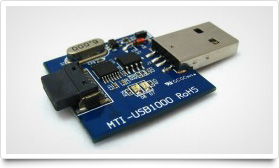
\includegraphics[scale=0.5]{Images/USB1000}
%\end{figure}
%
%\begin{table}[H]
%	\centering
%	\begin{tabularx}{\linewidth}{| l | l | X |}
%	\hline
%	\textbf{Item} & \textbf{Specification} & \textbf{Description} \\
%	\hline
%	\hline
%
%	\multicolumn{3}{|l|}{\textbf{Components}} \\
%	\hline
%	Interface Type & USB type A & USB 1.1 compatible. USB full speed support (12Mbps)\\
%	\hline
%	USB2UART Chip & FTDI\textregistered~ FT232BM & USB2UART converter chip\\
%	\hline
%	1kbit EEPROM & Microchip\textregistered~ 93C46 & Driver ID storage\\
%	\hline
%	Quad Buffer & Texas Instruments\textregistered~ SN74HC126 & USB Rx/Tx Communications buffer\\
%	\hline
%	Octal Switch & Analog Devices\textregistered~ ADG715 & Reset sequence recognition\\
%	\hline
%	Mote Interface & Terminal Block (ERNI\textregistered~ compatible) & Connector to CMXX00 WSN Motes (Vcc, GND, 8 port ADC, 2 port GPIO pins)\\
%	\hline
%
%	\end{tabularx}
%	\caption{Specifications for the USB1000 Interface Board \cite{USB1000}}
%	\label{tab:USB1000-spec}
%\end{table}
%
%\clearpage

\subsection{Sensor Board: CM5000}

\begin{figure}[H]
\centering
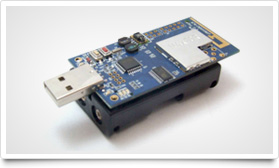
\includegraphics[scale=0.5]{Images/CM5000}
\end{figure}

\begin{table}[H]
	\centering
	\begin{tabularx}{\linewidth}{| l | l | X |}
	\hline
	\textbf{Item} & \textbf{Specification} & \textbf{Description} \\
	\hline
	\hline

	\multicolumn{3}{|l|}{\textbf{Processor}} \\
	\hline
	\multirow{2}{*}{Processor Model} & Texas Instruments\textregistered & Texas Instruments\textregistered\\
	~ & MSP430F1611 & MSP430 family\\
	\hline
	\multirow{3}{*}{Memory} & 48KB & Program Flash \\
	~ & 10KB & Data RAM \\
	~ & 1MB & External Flash (ST\textregistered~ M25P80) \\
	\hline
	ADC & 12bit resolution & 8 channels \\
	\hline
	\multirow{2}{*}{Interfaces} & UART, SPI, I2C & Serial Interfaces \\
	~ & USB & External System Interface (FTI\textregistered~ FT232BM) \\
	\hline
	\hline

	\multicolumn{3}{|l|}{\textbf{Radio}} \\
	\hline
	RF Chip & Texas Instruments\textregistered~ CC2420 & IEEE 802.15.4 2.4GHz Wireless Module\\
	\hline
	Frequency Band & 2.4GHz \mytilde 2.485GHz & IEEE 802.15.4 compliant \\
	\hline
	Sensitivity & -95dBm typ & Receive Sensitivity \\
	\hline
	Transfer Rate & 250Kbps & IEEE 802.15.4 compliant \\
	\hline
	RF Power & -25dBm \mytilde 0dBm & Software Configurable \\
	\hline
	\multirow{2}{*}{Range} & \mytilde120m (outdoor) & \multirow{2}{5cm}{Longer ranges possible with optional SMA antenna attached} \\
	~ & 20~\mytilde30m (indoor) & ~ \\
	\hline
	\multirow{3}{*}{Current Draw} & RX: 18.8mA & \multirow{3}{5.5cm}{Lower RF Power Modes reduce consumption} \\
	~ & TX: 17.4mA & ~ \\
	~ & Sleep mode: 1uA & ~ \\
	\hline
	RF Power Supply & 2.1V \mytilde 3.6V & CC2420 Input Power \\
	\hline
	Antenna & Dipole Antenna / PCB Antenna & Additional SMA connector available for extra antenna \\
	\hline
	\hline

	\multicolumn{3}{|l|}{\textbf{Sensors}} \\
	\hline
	Light 1 & Hamamatsu® S1087 Series & Visible Range (560 nm peak sensitivity wavelength)\\
	\hline
	Light 2 & Hamamatsu® S1087 Series & Visible \& Infrared Range (960 nm peak sensitivity wavelength)\\
	\hline
	\multirow{6}{2.5cm}{Temperature \& Humidity} &  \multirow{6}{*}{Sensirion® SHT11} & Temperature Range: -40 \mytilde 123.8 $^\circ$C  \\
	~ & ~ & Temperature Resolution: $\pm$ 0.01 (typical) \\
	~ & ~ & Temperature Accuracy: $\pm$ 0.4 $^\circ$C (typical) \\
	~ & ~ & Humidity Range: 0 \mytilde 100\% RH \\
	~ & ~ & Humidity Resolution: 0.05 (typical) \\
	~ & ~ & Humidity Accuracy: $\pm$ 3 \%RH (typical) \\
	\hline

	\end{tabularx}
	\caption{Specifications for the CM5000 Wireless Sensor Node \cite{CM5000}}
	\label{tab:CM5000-spec}
\end{table}


\clearpage

\subsection{Network Infrastructure: UD1000}

\begin{figure}[H]
\centering
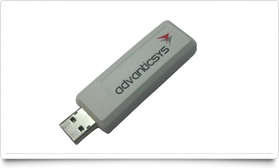
\includegraphics[scale=0.5]{Images/UD1000}
\end{figure}

\begin{table}[H]
	\centering
	\begin{tabularx}{\linewidth}{| l | l | X |}
	\hline
	\textbf{Item} & \textbf{Specification} & \textbf{Description} \\
	\hline
	\hline

	\multicolumn{3}{|l|}{\textbf{Processor}} \\
	\hline
	Processor Model & Texas Instruments\textregistered~ MSP430F1611 & Texas Instruments\textregistered~ MSP430 family\\
	\hline
	\multirow{2}{*}{Memory} & 48KB & Program Flash \\
	~ & 10KB & Data RAM \\
	\hline
	ADC & 12bit resolution & 8 channels \\
	\hline
	\multirow{2}{*}{Interfaces} & UART, SPI, I2C & Serial Interfaces \\
	~ & USB & External System Interface (FTI\textregistered~ FT232BM) \\
	\hline
	\hline

	\multicolumn{3}{|l|}{\textbf{Radio}} \\
	\hline
	RF Chip & Texas Instruments\textregistered~ CC2420 & IEEE 802.15.4 2.4GHz Wireless Module\\
	\hline
	 Frequency Band & 2.4GHz \mytilde 2.485GHz & IEEE 802.15.4 compliant \\
	\hline
	Sensitivity & -95dBm typ & Receive Sensitivity \\
	\hline
	Transfer Rate & 250Kbps & IEEE 802.15.4 compliant \\
	\hline
	RF Power & -25dBm \mytilde 0dBm & Software Configurable \\
	\hline
	Range & \mytilde40m (outdoor), 15\mytilde20m (indoor) & Dongle orientation dependent \\
	\hline
	\multirow{3}{*}{Current Draw} & RX: 18.8mA & \multirow{3}{4.5cm}{Lower RF Power Modes reduce consumption} \\
	~ & TX: 17.4mA & ~ \\
	~ & Sleep mode: 1uA & ~ \\
	\hline
	RF Power Supply & 2.1V \mytilde 3.6V & CC2420 Input Power \\
	\hline
	Antenna & Ceramic antenna & ~ \\
	\hline
	\hline

	\multicolumn{3}{|l|}{\textbf{Electromechanical Characteristics}} \\
	\hline
	Dimensions & 65mm x 22.5mm x 14mm & Including housing\\
	\hline
	Weight & 15g & ~\\
	\hline
	Power & 5V  & DC over USB\\
	\hline
	Current & 90mA  & Max rated current over USB\\
	\hline
	Operating Temperature & -25$^\circ$C \mytilde +60$^\circ$C & ~\\
	\hline
	Storage Temperature & -40$^\circ$C \mytilde +60$^\circ$C & ~\\
	\hline
	Operating Humidity & 5\% \mytilde 95\% & Non condensing\\
	\hline
	Protection type & IP20 & Non condensing\\
	\hline

	\end{tabularx}
	\caption{Specifications for the UD1000 Sensor Network Sink \cite{UD1000}}
	\label{tab:UD1000-spec}
\end{table}


\newpage

\section{2420 Power-Distance Results}

\begin{table}[H]
	\centering
	\begin{tabular}{ | l | l | }
		\hline
		Power level & Ave. Maximum Distance \\
		\hline
		1 & 10cm \\
		2 & 21cm \\
		3 & 85cm \\
		4 & ~ \\
		5 & ~ \\
		6 & ~ \\
		7 & ~ \\
		8 & ~ \\
		9 & ~ \\
		10 & ~ \\
		11 & ~ \\
		12 & ~ \\
		13 & ~ \\
		14 & ~ \\
		15 & ~ \\
		16 & ~ \\
		17 & ~ \\
		18 & ~ \\
		19 & ~ \\
		20 & ~ \\
		21 & ~ \\
		22 & ~ \\
		23 & ~ \\
		25 & ~ \\
		26 & ~ \\
		27 & ~ \\
		28 & ~ \\
		29 & ~ \\
		30 & ~ \\
		31 & ~ \\
		\hline
	\end{tabular}
	\caption{The distance nodes could communicate at different power levels set by $cc2420\_set\_txpower$}
\end{table}

\newpage

\section{Algorithm Implementation}

%\subsection{Tree Aggregation}

%\inputminted[linenos=true,tabsize=3,fontsize=\small]{c}{../Samples/TreeAggregator/tree-aggregator.c}

%\subsection{Clustering}

%\inputminted[linenos=true,tabsize=3,fontsize=\small]{c}{../Samples/Clustering/cluster.c}

\newpage


\section{References}
\renewcommand{\refname}{\vspace{-1cm}}
\bibliographystyle{myplainnat}
\bibliography{../References/references,../References/BradburyCS310}


\end{document}
